%!TEX root = ../thesis.tex
%*******************************************************************************
%****************************** Third Chapter **********************************
%*******************************************************************************
\chapter{Applications}

% **************************** Define Graphics Path **************************
\ifpdf
    \graphicspath{{Chapter3/Figs/Raster/}{Chapter3/Figs/PDF/}{Chapter3/Figs/}}
\else
    \graphicspath{{Chapter3/Figs/Vector/}{Chapter3/Figs/}}
\fi

In the first two chapters I have provided an overview of the theoretical basis of my work and placed it within the history of related approaches.
Here, I will demonstrate how the methods I develop can aid biological insight in a number of species domains.
To do so, I will use methods described in chapter 2 as implemented in {\tt vg}.

The small genome of \emph{Saccharomyces cerevisiae} and ready availability of sources for pangenomic data models made it very useful to my development of {\tt vg}.
I begin by illustrating this for a variety of pangenome constructions and also a variety of read lengths.

However, much interest in bioinformatics is with larger genomes, specifically human.
I use evaluations based on the human genome to validate the ability of {\tt vg} to scale to large genomes.
Through simulation and the analysis of real genomes, I show that the aligner I implement, {\tt vg map}, yields the same quality of alignment as {\tt bwa mem} against linear genomes.
Although {\tt vg map}'s runtime is between five to ten-fold slower than {\tt bwa mem}, it provides improved, less biased alignment against variation graphs.
I develop a variation graph for the reference-guided genome assemblies from the HGSVC project and demonstrate the strong effect of reference bias in ChIP-seq data.

One context where reference bias has very significant effects is in the analysis of ancient DNA (aDNA).
Here short reads and high intrinsic error rates encourage a high rate of reference bias.
I show that alignment against a pangenome graph ameliorates this issue.

{\tt vg} can be applied to any kind of variation graph.
To demonstrate the utility of this, I use de Bruijn assemblers to generate reference variation graphs from collections of raw sequencing reads in the absence of a prior reference.
I recreate a classical pangenomic analysis of core and accessory pangenome by analyzing the coverage of alignments mapped to an assembly graph built from 10 \emph{Escheria coli} strains.
To illustrate the application of vg to metagenomic data containing unknown source genomes, I show that {\tt vg} enables the full length alignment of reads to a complex assembly graph built from an arctic viral metagenome, and similarly improves alignment to an assembly graph built from a human gut microbiome.
Finally, I demonstrate that the data models and indexes in {\tt vg} are capable of encoding splicing graphs, and that aligning to these splicing graphs allows the direct observation of the transcriptome.

\section{Yeast}
%*0.5p 0.5h*

\emph{Saccharomyces cerevisiae}, commonly known as baker's or brewer's yeast due to its gastronomic applications, has long been among the most important model organisms in biology, and its small genome attracted some of the first population scale whole genome surveys of variation to be undertaken using low-cost sequencing.
The genome of \emph{S. cerevisiae} was the first eukaryotic genome sequenced, in 1996 \cite{goffeau1996life}.
Resequencing studies followed that used \emph{cerevisiae} as a model system to understand genome evolution.
The Saccharomyces Genome Resequencing Project (SGRP) \cite{liti2009population}, which used low-coverage capillary Sanger sequencing to generate a population survey for \emph{cerevisiae} can be seen as a precursor to the 1000GP, in its use of low-coverage sequencing and imputation to establish the panel\footnote{\url{https://www.sanger.ac.uk/research/projects/genomeinformatics/assets/sgrp_manual.pdf}}.
A followup project, the SGRP2, used resequencing and whole genome assembly of high coverage, low cost Illumina sequencing to establish that the greater phenotypic diversity in \emph{S. cerevisiae} relative to its wild relative \emph{S. paradoxus} is likely due to structural variation (as measured by presence/absence and copy number) rather than SNP diversity \cite{bergstrom2014high}.
Recently, whole genome \emph{de novo} assembly with long single-molecule reads has further refined this conclusion by demonstrating that the structural diversity is non-uniformly distributed throughout the genomes of \emph{S. cerevisiae}, concentrating in subtelomeric regions \cite{yue2017contrasting}.
In this section, I use data from independent sequencing of the UK's National Center for Yeast Collections (NCYC) as well as long reads from \cite{yue2017contrasting} to demonstrate the capabilities of {\tt vg} and compare the utility of various variation graph models built from these population surveys.

\subsection{A SNP-based SGRP2 graph}
\label{sec:SGRP2_graph}
%*1p 1h*T
%I consider only \emph{S. cerevisiae}, using the SGD reference genome and the SNP variation results from the SGRP2.
The earliest rigorous testing of {\tt vg}'s alignment method was against a variation graph constructed from the SGRP2's released VCF for \emph{S. cerevisiae}\footnote{\url{http://www.moseslab.csb.utoronto.ca/sgrp/data/SGRP2-cerevisiae-freebayes-snps-Q30-GQ30.vcf.gz}}.
This early population resequencing project produced a VCF including only SNPs, yet using it already presented problems typical even when working with larger scale genomes.
The transposable elements in the genome generate rich patterns of repeats which make alignment difficult and require the development of mapping quality.
Dense variation is also present in the results and this necessitates the application of pruning strategies to the graph to mask out high-complexity regions for indexing.
Mistakes in the mapper could be readily observed and testing could easily be done on a laptop, whereas larger genomes require longer runtimes for indexing and larger servers in order to support the indexes during alignment.

The SGRP2 graph can be built and indexed in around 10 minutes on a commodity compute server, including the construction of the GBWT index and the generation of an order-256 GCSA2 index using a pruned and refilled version of the graph.
It contains exactly the number of bases in the SGD\_2010 reference plus the number of SNP alternate alleles in the SGRP2 VCF: 12163423 + 243629 = 12407052.
The graph itself uses 23MB on disk, in contrast to that of the SGD\_2010 reference, which takes only 7.6MB.
Much of this difference is due to the larger number of entities required by to represent the variation-containing graph.
The SGD\_2010 graph is linear, with a gap for each chromosome, and contains 380,115 nodes and 380,097 edges after splitting into nodes of typical size 32bp, while the SGRP2 graph contains SNPs and is represented with 714,533 nodes and 969,690 edges.
Note that by default, GCSA2 indexing works on nodes with a maximum length less than 1024, and {\tt vg map} performs better if the maximum node size is limited further, with 32bp usually the standard maximum length in experiments I will present here.
The resulting indexes also differ in size, with the SGRP2 graph's {\tt xg} index requiring 71MB, while the SGD\_2010 graph's only 38MB.
The full GCSA index for the SGRP2 graph is substantially larger, at 220MB, in contrast to only 50MB for the linear reference, which reflects the greater complexity required to include all the recombination in the pruned and haplotype re-filled graph used for indexing.

To validate that the SGRP2 reference is a closer match to real read sets, I then mapped subsets of reads from \emph{cerevisiae} samples that were in the NCYC collection but were not part of SGRP2.
I aligned 100K read pairs from each of 12 samples ($N=2.4$M total reads) to both the SGD\_2010 reference graph and the SGRP2 pangenome graph.
For each read, we can compare the alignment score and identity between the two graphs to evaluate the gain provided by using the pangenome as a reference.
When we map the real reads from new strains not used to build the graph, 24.5\% of the reads map better to the pangenome than to the linear reference (figure \ref{fig:NCYC_SGD_SGRP2}).
A small fraction of reads (0.46\%) map better to the linear than to the pangenome graph, which could result from changes in paired alignment rescue, the effects of the pruning process, the slightly different minimum MEM size calculated for the two graphs, or errors in the SGRP2.
%Although differences in the relative benefit of using the SGRP2 pangenome appear between samples, they are minor and not apparently systematic (Figures \ref{subfig:NCYC_score_diff_hist} and \ref{subfig:NCYC_id_diff_hist}).

\begin{figure}[htbp!] 
  \centering
  \begin{subfigure}[t]{0.49\textwidth}
    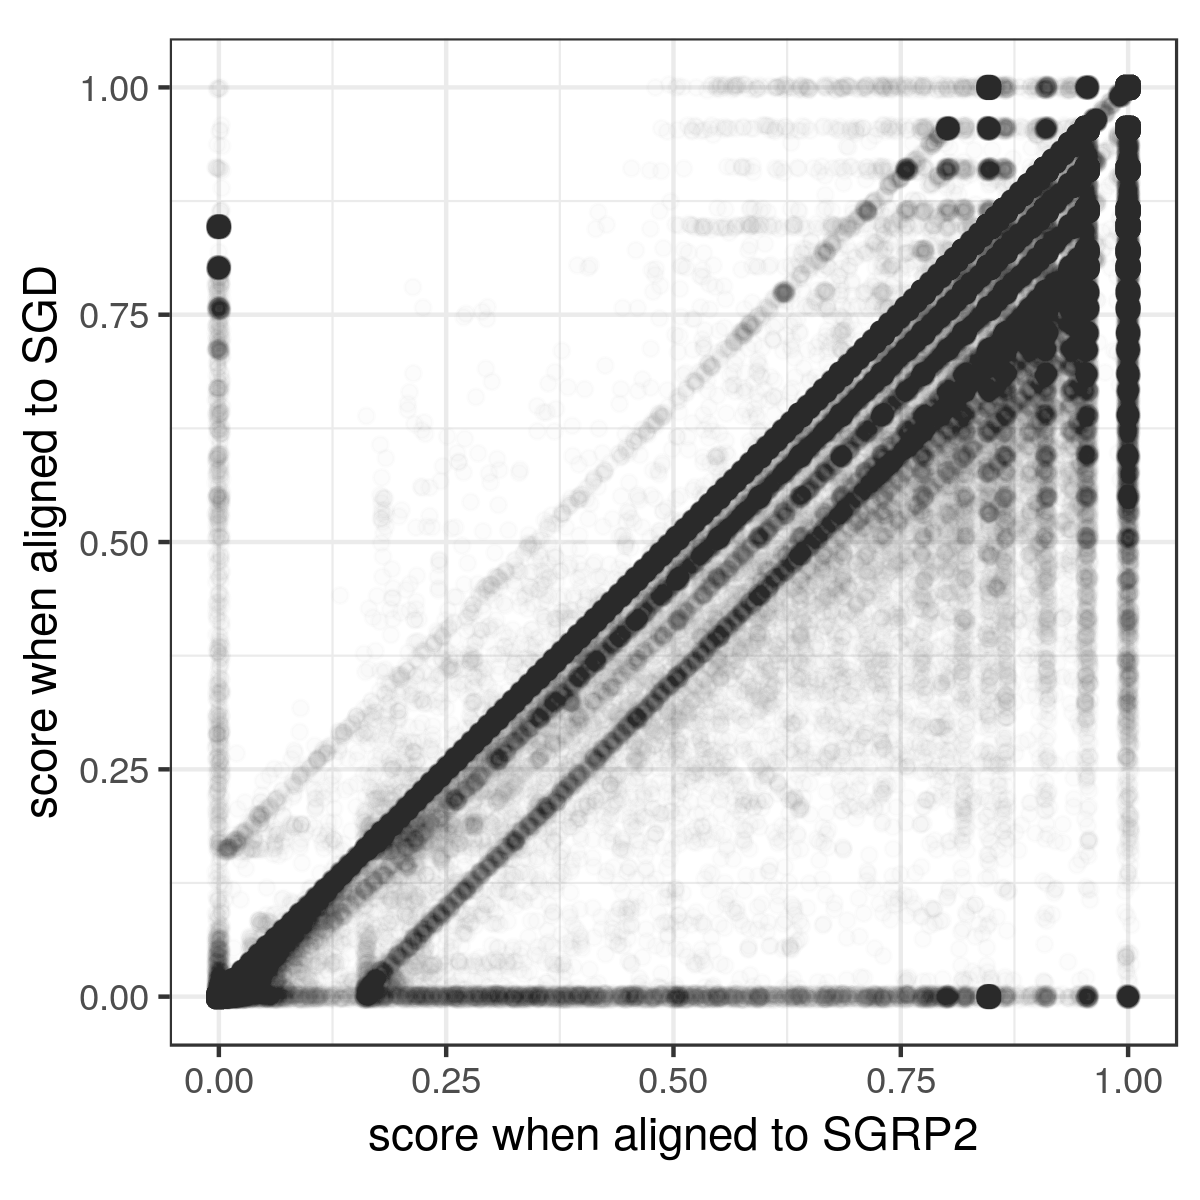
\includegraphics[width=1.0\textwidth]{Chapter3/Figs/NCYC_SGRP2_SGD_comparison_score.png}
    \caption{Alignment score} \label{subfig:NCYC_score}
  \end{subfigure}
  \begin{subfigure}[t]{0.49\textwidth}
    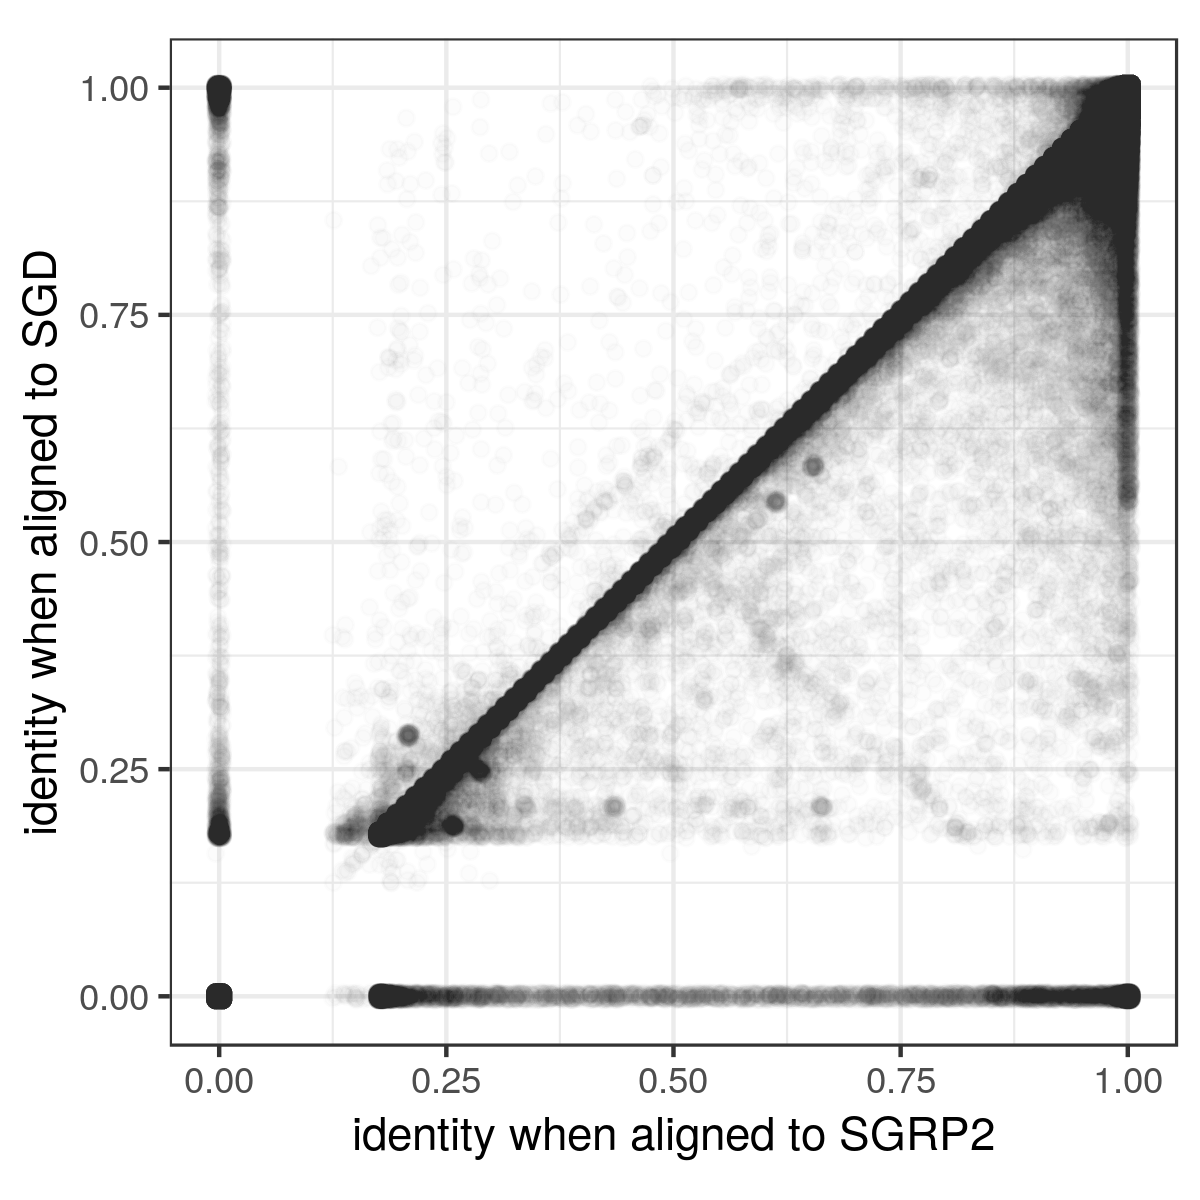
\includegraphics[width=1.0\textwidth]{Chapter3/Figs/NCYC_SGRP2_SGD_comparison_id.png}
    \caption{Alignment identity} \label{subfig:NCYC_identity}
  \end{subfigure}
  \begin{subfigure}[t]{1.0\textwidth}
    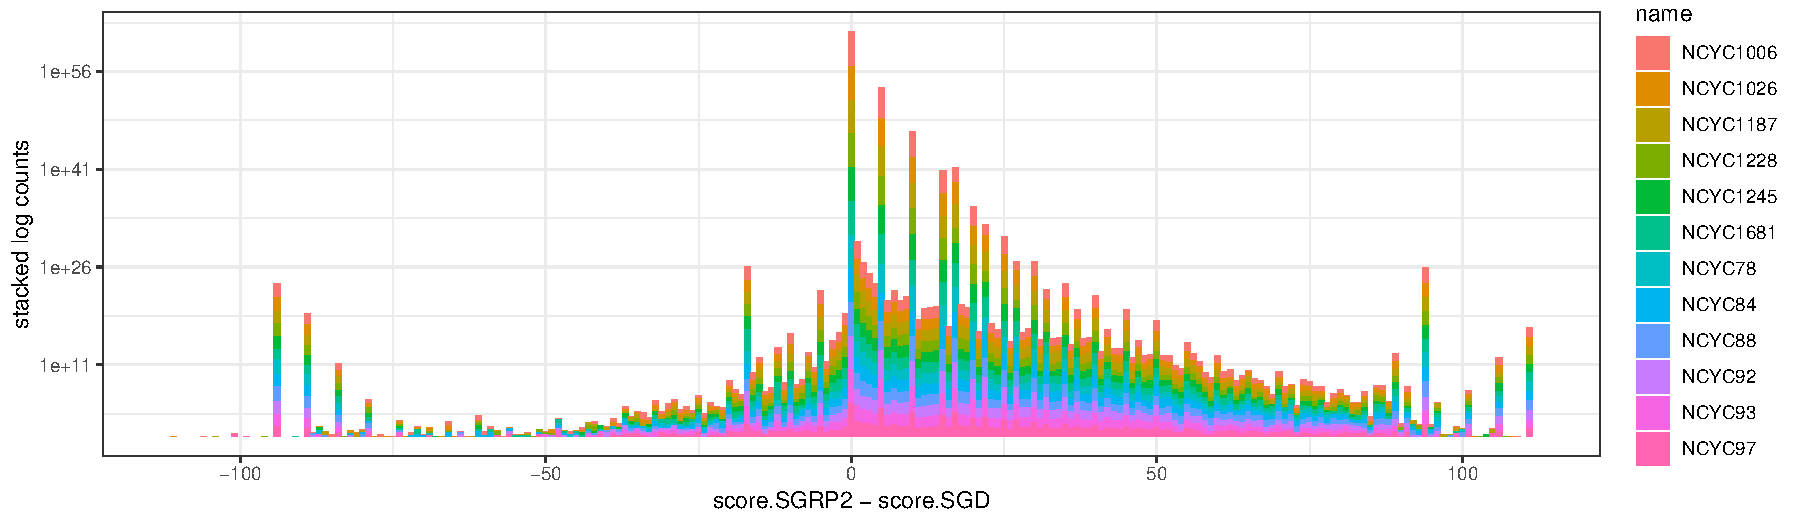
\includegraphics[width=1.0\textwidth]{Chapter3/Figs/NCYC_SGRP2_SGD_comparison_score_hist_color.pdf}
    \caption{Difference in alignment score} \label{subfig:NCYC_score_diff_hist}
  \end{subfigure}
  \begin{subfigure}[t]{1.0\textwidth}
    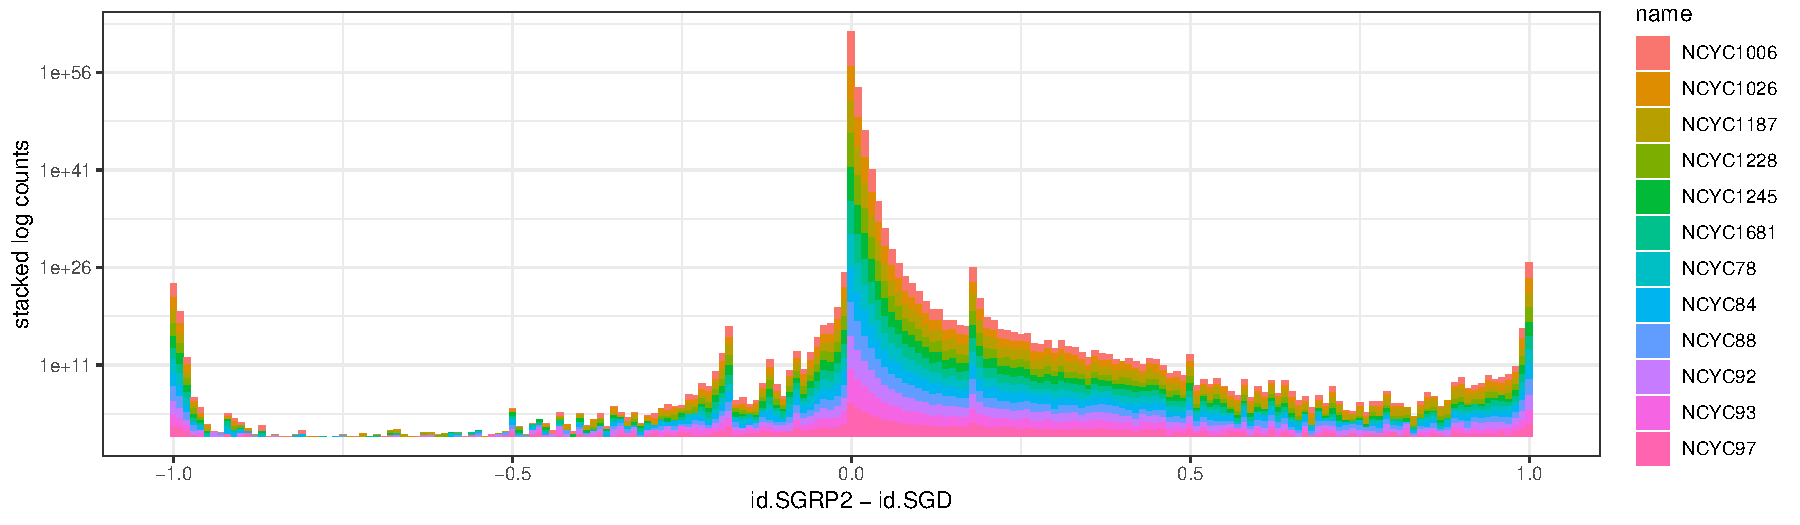
\includegraphics[width=1.0\textwidth]{Chapter3/Figs/NCYC_SGRP2_SGD_comparison_id_hist_color.pdf}
    \caption{Difference in alignment identity} \label{subfig:NCYC_id_diff_hist}
  \end{subfigure}
  \caption[Comparing alignment to the linear reference and SGRP2]{
    Alignment of 100k read pairs from 12 NCYC \emph{S. cerevisiae} strains against the SGD\_2010 reference genome (SGD) or the SGRP2 pangenome (SGRP2).
    In (\ref{subfig:NCYC_score}) alignment scores are plotted for each read.
    The shift in density to the right relative to $y=x$ indicates improved alignments to the pangenome.
    In (\ref{subfig:NCYC_identity}) we observe the same pattern when using alignment identity rather than score.
    Subfigures \ref{subfig:NCYC_score_diff_hist} and \ref{subfig:NCYC_id_diff_hist} provide a stacked log-scaled histogram of the difference in score and identity between the two graphs.
    Note that the $y$-axes in these histograms represent the stacking of the log-transformed groups, which ensures that the relative width of each group's band is not distorted by its order in the plotting.
  }
\label{fig:NCYC_SGD_SGRP2}
\end{figure}

\subsection{Cactus progressive assembly}
%*0.5p 0.5h*
\label{sec:yeast_cactus}

Variation graphs are generic objects capable of representing any kind of alignment between genomes or assembly of read data from them.
To test the ability of {\tt vg} to use graphs of complex topology, we constructed a whole genome alignment graph of \emph{de novo} assemblies produced from PacBio sequencing of seven strains of \emph{S. cerevisiae}.
In this assembly each chromosome of each assembly in \cite{yue2017contrasting} was progressively aligned using the phylogenetic guide tree methodology implemented in Cactus \cite{Paten:2011fva}.
As illustrated in figure \ref{fig:cactus_yeast_zoom}, this graph encodes a complex global topology that captures the structural variation between the species also reported in \cite{yue2017contrasting} as well as a local DAG-like topology which we expect when homologous sequences are represented compactly in a graph.
This illustrates the ability of vg to represent paths corresponding to both collinear (inset) and structurally rearranged (main figure) regions of genomic variation.

\begin{figure}[htbp!]
  \centering
  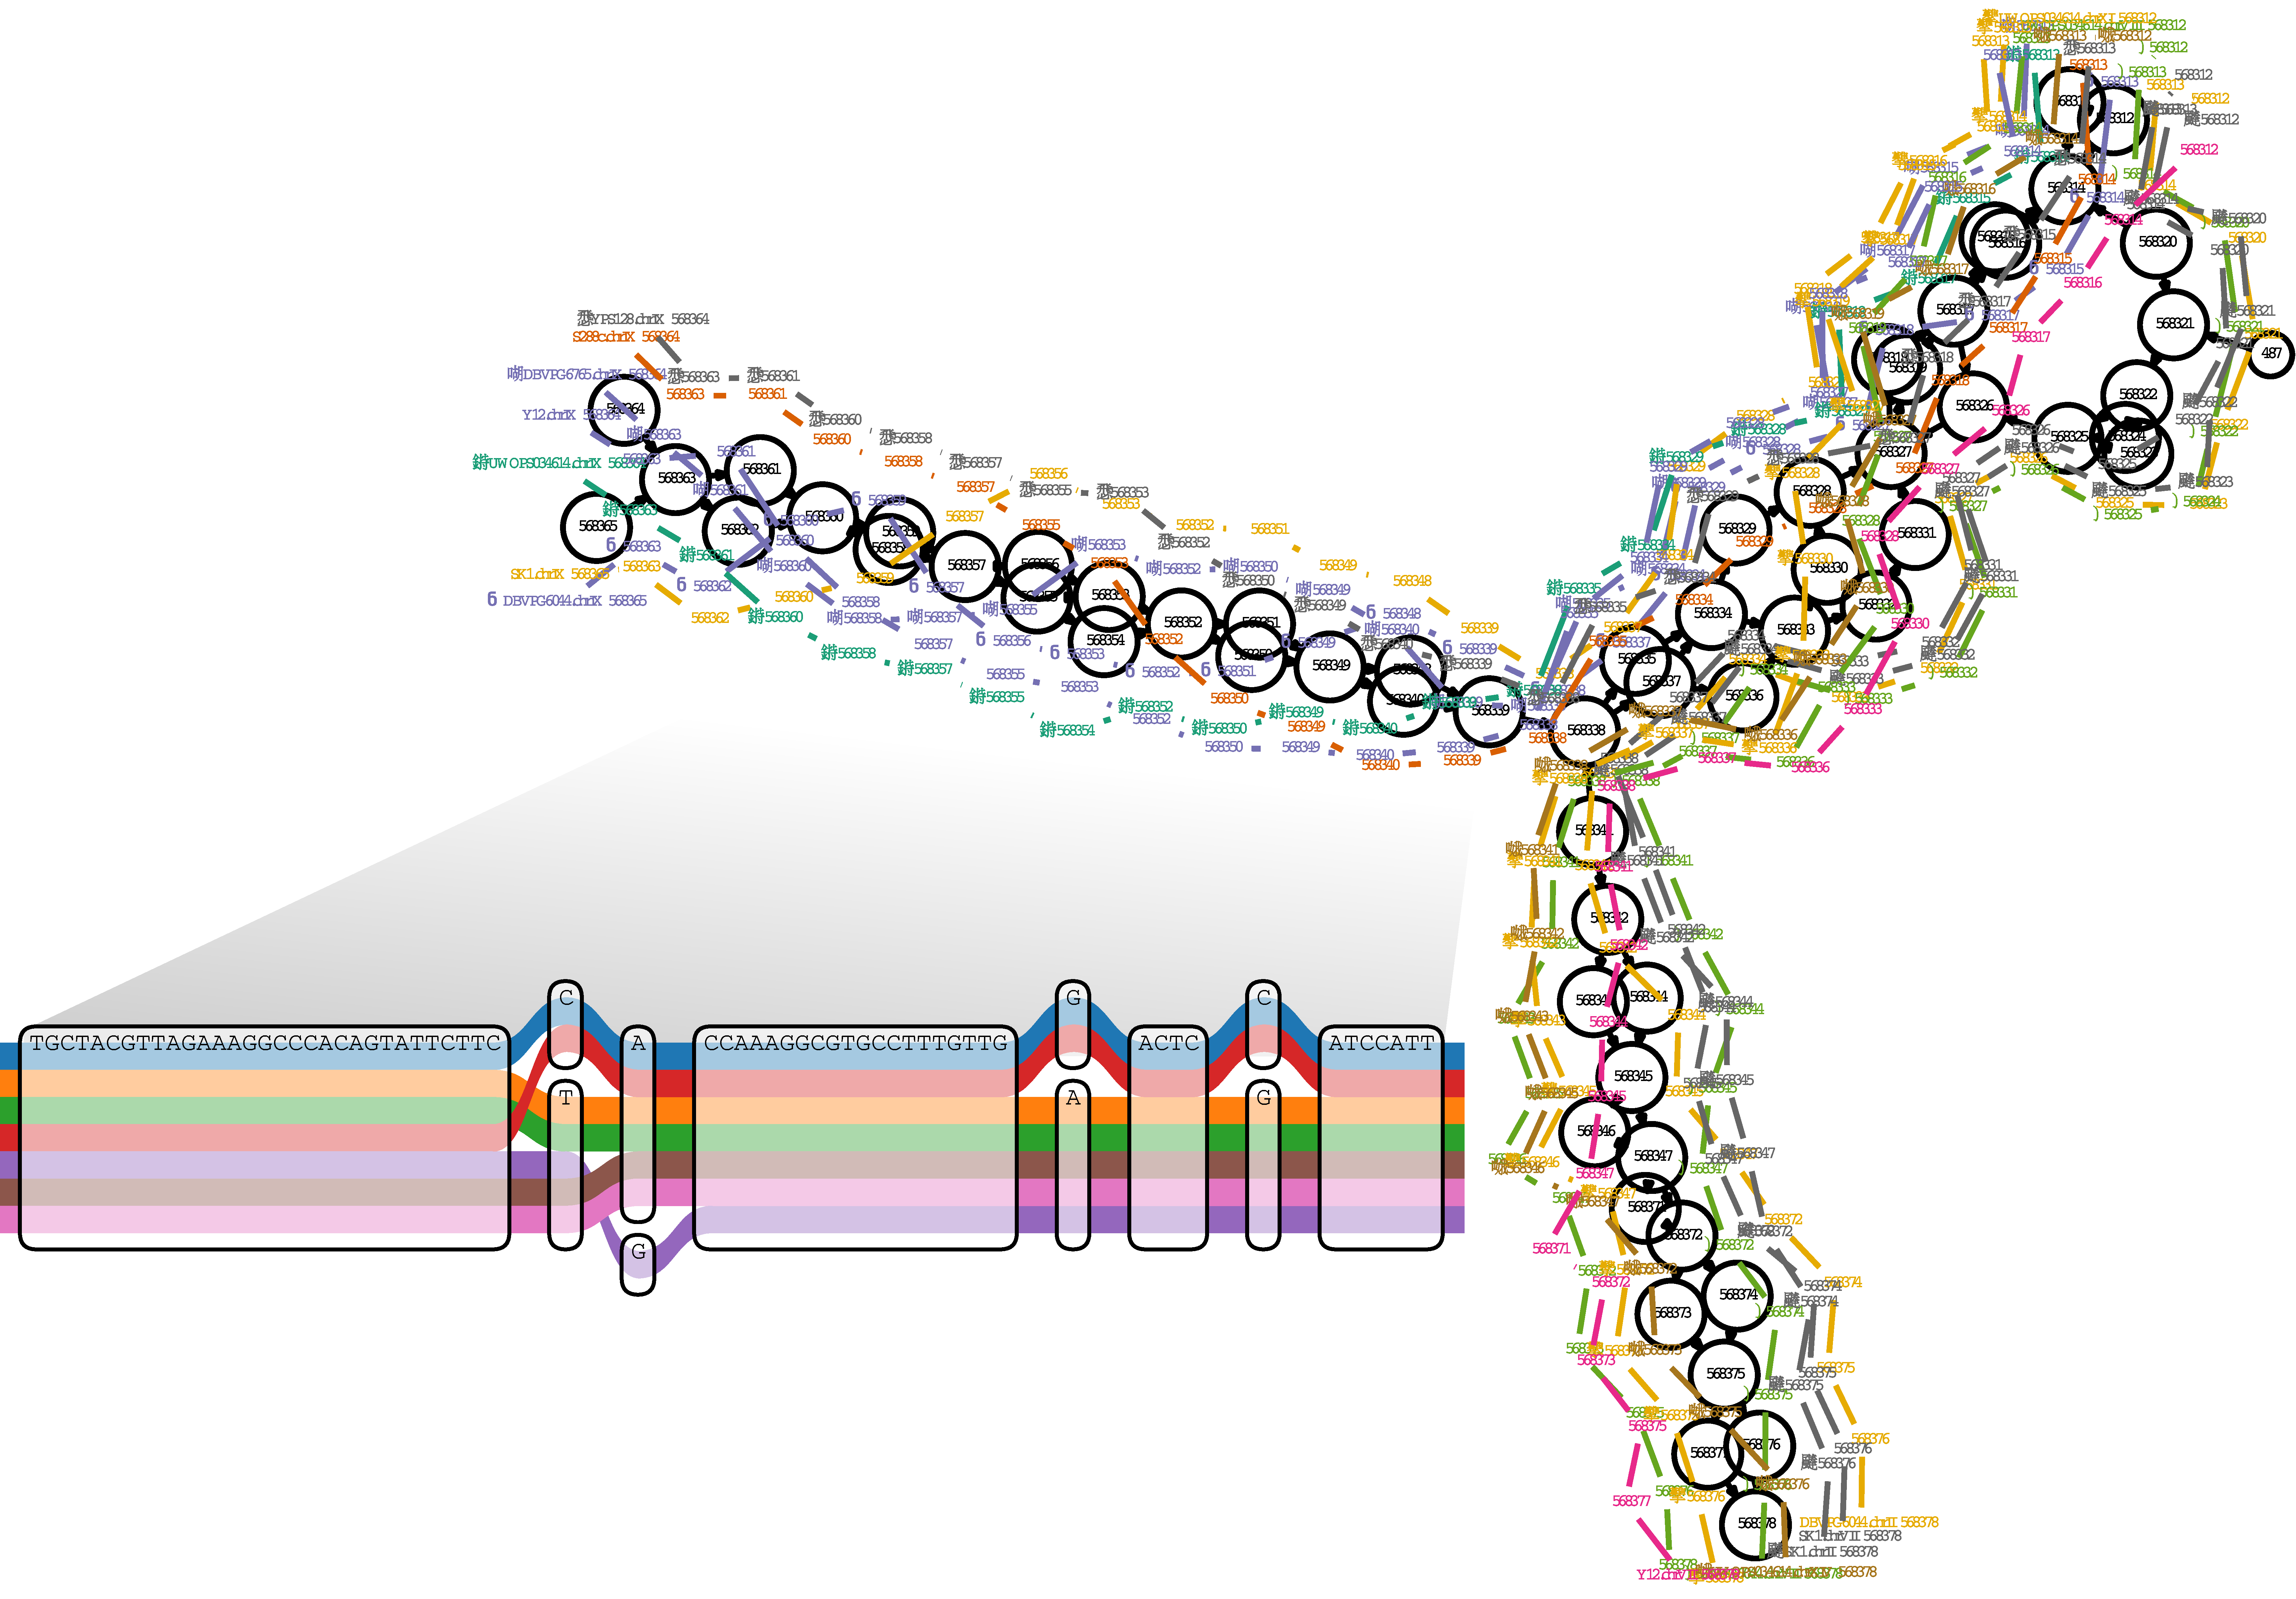
\includegraphics[width=1.0\textwidth]{Chapter3/Figs/cactus_yeast_zoom.pdf}
  \caption[Cactus yeast variation graph]{
  A region of a yeast genome variation graph.
  This displays the start of the subtelomeric region on the left arm of chromosome 9 in a multiple alignment of the strains sequenced in \cite{yue2017contrasting} as assembled by Cactus \cite{Paten:2011fva}.
  The inset shows a subregion of the alignment at single-base level.
  The colored paths correspond to separate contiguous chromosomal segments of these strains.
  Reprinted from \cite{garrison2018variation}.
  }
  \label{fig:cactus_yeast_zoom}
\end{figure}

A simulation study based on the SK1 strain provides some insight into the capabilities of {\tt vg} and tradeoffs inherent in different graph designs.
I compared four vg graphs: a linear reference graph from the standard S288c strain, a linear reference from the SK1 strain, a pangenome graph of all seven strains, and a ``drop SK1'' variation graph in which all sequence private to the strain SK1 was removed from the pangenome graph.
The multiple genome graphs were constructed with the Cactus progressive aligner, which generates graphs that typically contain cycles and are not partially ordered, and then filtered down to the various subgraphs using path subsetting facilities in {\tt vg mod}.

\begin{figure}[htbp!]
  \centering
  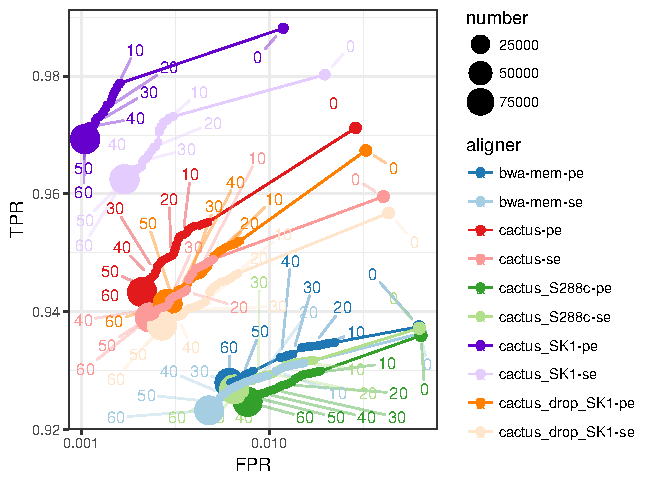
\includegraphics[width=1.0\textwidth]{Chapter3/Figs/e68fc338_test_sim_yeast_cactus-roc.pdf}
  \caption[Cactus yeast simulation]{Mapping short reads with vg to yeast genome references.
    ROC curves obtained by mapping 100,000 simulated SK1 yeast strain 150-bp paired-end reads against a variety of references described in the text.
    Reprinted from \cite{garrison2018variation}.}
  \label{fig:cactus_yeast_sim}
\end{figure}


We simulated 100,000 150-bp paired-end reads from the SK1 reference, modeling sequencing errors, and mapped them to the four references (ROC curves, Figure \ref{fig:cactus_yeast_sim}).
Not surprisingly, the best performance was obtained by mapping to a linear reference of the SK1 strain from which the data were simulated, with substantially higher sensitivity and specificity compared to mapping to the standard linear reference from the strain S288c with either {\tt vg} or {\tt bwa mem}.
Mapping to the variation graphs gave intermediate performance, with >1\% more sensitivity and lower false-positive rates than mapping to the standard reference.
There was surprisingly little difference between mapping to graphs with and without the SK1 private variation, probably because much of what is novel in SK1 compared to the reference is also seen in other strains.
Mapping to either graph had lower sensitivity compared to mapping just to the SK1 sequence, likely because of suppression of GCSA2 index $k$-mers in complex or duplicated regions, which our indexing strategy was not designed to address.

\subsection{Constructing diverse \emph{cerevisiae} variation graphs}
\label{sec:constructing_yeast_graphs}

With {\tt vg}, our goal is to build a toolkit that allows the use of any genome graph as a reference.
To validate this capability, I used data sources for \emph{S. cerevisiae} to build seven variation graphs, whose dimensions are listed in table \ref{table:yeast_graphs}.
In the next section (\ref{sec:yeast_long_read}) I present an evaluation of these graphs using long reads from the SK1 strain.


\begin{table}[h]
  \centering
\begin{tabular}{l||c|c|c|c|c}
\itshape name & \itshape size (MB) & \itshape length & \itshape nodes & \itshape edges & \itshape subgraphs \\
\hline
SGD\_2010 & 7.3 & 12163423 & 380115 & 380097 & 18 \\
S288c & 7.3 & 12249246 & 382797 & 382781 & 18 \\
SGRP2 & 21 & 12407052 & 714533 & 969690 & 18 \\
minia unitigs & 15 & 14419206 & 1232804 & 1332994 & 46131 \\
minia contigs & 6.4 & 12233279 & 421125 & 425683 & 2961 \\
Cactus & 31 & 13243056 & 1059173 & 1304205 & 580 \\
{\tt vg msga} & 42 & 13793955 & 1156295 & 1387903 & 2 \\
\hline
\end{tabular}
\caption[\emph{S. cerevisiae} variation graphs]{
  A summary of seven different variation graphs constructed to represent variation in \emph{S. cerevisiae}.
  As described in section \ref{sec:SGRP2_graph}, the SGD\_2010 graph is built from the reference, while SGRP2 adds SNPs in the SGRP2 population survey.
  The Illumina data from \cite{yue2017contrasting} was used to build the minia unitigs and minia contigs graphs, while the whole genome, chromosome-resolved PacBio assemblies from the same work were used to build the Cactus and {\tt vg msga} progressive assemblies.
  S288c is the \emph{de novo} assembly of the reference strain produced in \cite{yue2017contrasting}.
}
\label{table:yeast_graphs}
\end{table}

Three of the graphs are effectively linear or DAG-like, except for their mitochondria and plasmid chromosomes, which are included as circular components.
SGD\_2010 and S288c represent two assemblies of the reference genome, the former from the SGD genome sequencing project, and the latter is a \emph{de novo} assembly from \cite{yue2017contrasting}.
The difference in quality between the two approaches will be made apparent in the subsequent section.
As described in section \ref{sec:SGRP2_graph}, the SGRP2 graph adds SNP variation from the population survey in \cite{bergstrom2014high} to build a pangenome reference.
The SGD\_2010 reference contains the mitochondria and 6kb plasmid sequence, while the S288c assembly excludes them due to the sequencing protocol, where size selection in the library preparation stage removed these short sequences, so to enable direct comparison in later tests these were added to the S288c graph.

The remaining four graphs are different forms of assembly graph.
Using the Illumina data published in \cite{yue2017contrasting}, I build two assemblies with minia3, using a $k$-mer size of 51 and a high abundance threshold (50) to limit the resulting graph complexity.
In the first, I take the unitig graph that represents all non-branching paths in the compacted DBG as nodes.
The second is the result of the minia contigification process that pops bubbles and cleans the graph to attempt to arrive at longer contigs.
Both results are expressed as overlap graphs in GFA, and I can import them as variation graphs using bluntification and graph pseudotopological sorting.
As shown in table \ref{table:yeast_graphs}, the unitig graph is considerably more complex in terms of node density than the contig graph.
It also contains more sequence, presumably because some regions that are separated in the unitig graph are collapsed in the contig graph.
The number of disjoint components in these graphs is very high (2961 for the contig graph and 46131 for the unitig graph), suggesting that pruning of the assembly graph has yielded a greatly fragmented result.
The resulting graphs are difficult to align long reads to.
I conclude that further tuning of the parameters used during \emph{de novo} assembly from short reads will be required to use assemblies like this as reference graphs.

Finally, I used the whole genome \emph{de novo} assemblies of long read data from \cite{yue2017contrasting} to build whole genome alignment graphs using Cactus (as described in section \ref{sec:yeast_cactus}) and {\tt vg msga}.
The multiple sequence to graph alignment (MSGA) process implemented in {\tt vg msga} is akin to the progressive POA method, but generalized to arbitrary graphs of any size.
Rather than using a local alignment algorithm to expand the graph, the long read alignment algorithm described in section \ref{sec:chunked_alignment} allows the direct alignment of whole chromosomes to the graph.
Where the Cactus progressive assembly uses a phylogenetic guide tree to structure its construction, {\tt vg msga} simply aligns the chromosomes in order from longest to shortest to the growing graph.
The long read alignment in {\tt vg} is structured to enforce long range synteny, and the resulting graph is substantially different in structure than that of Cactus.
I find that {\tt vg msga} is less likely to collapse repeats than Cactus, at least in the configuration used for this assembly.
We can see this in figure \ref{fig:yeast_bandage}, where the Cactus graph (\ref{subfig:cactus_yeast_bandage}) shows two dense repeat structures in its core connected by loops of unique sequence, while the {\tt vg msga} graph appears to have much longer loops, with collapsed repeats embedded in these loops.
This observation is supported by the length statistics in table \ref{table:yeast_graphs}, with {\tt vg msga} producing a graph that is 550,899bp longer than that of Cactus.
At the same time, the node count of the {\tt vg msga} graph is higher, which perhaps reflects a different local alignment result.

\begin{figure}[htbp!]
  \begin{subfigure}[t]{0.9\textwidth}
    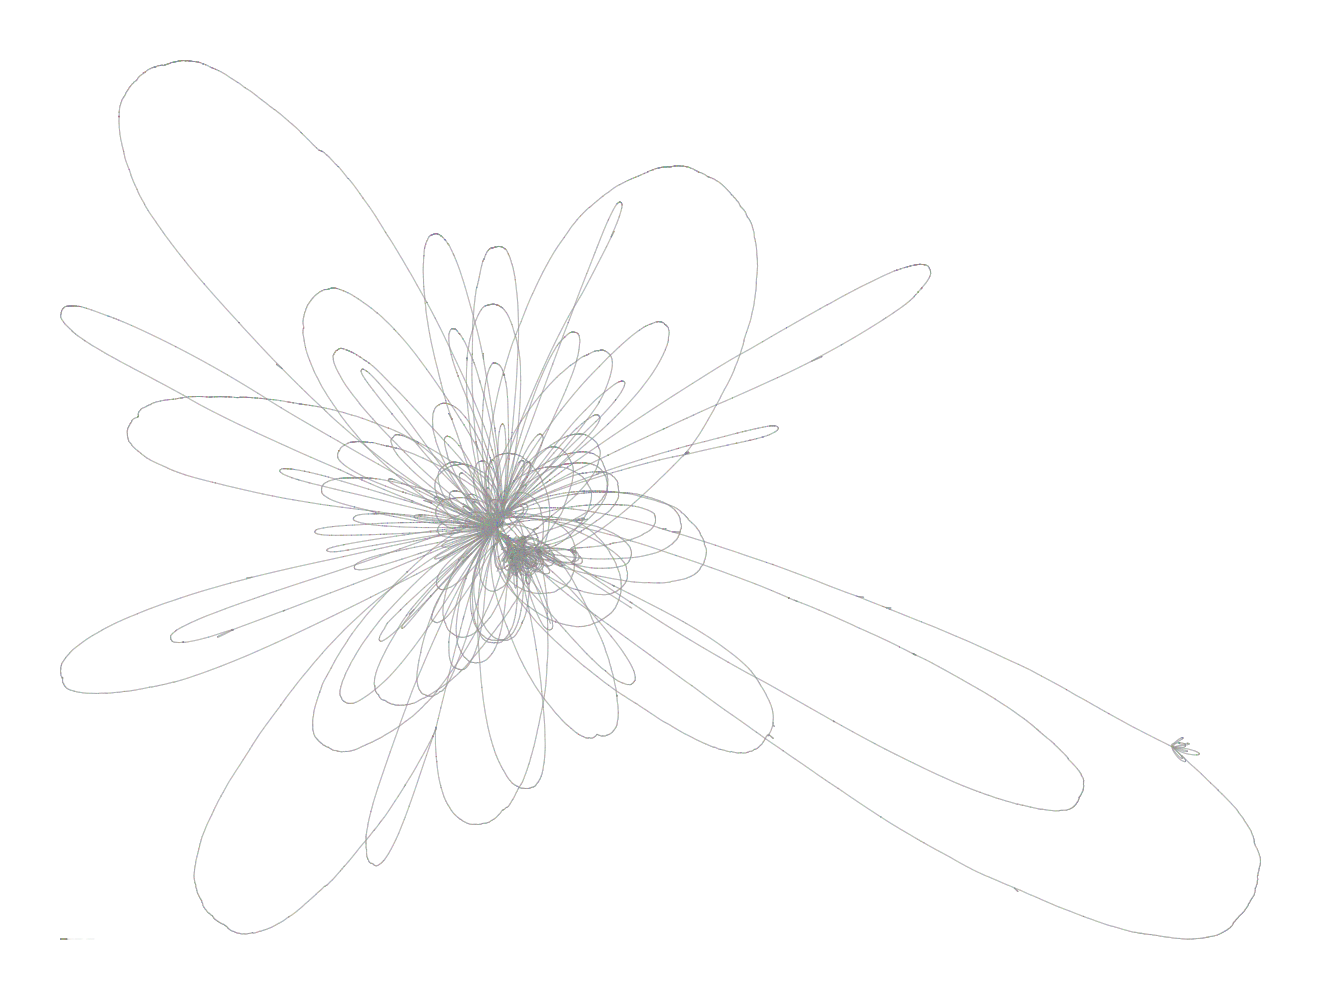
\includegraphics[width=1.0\textwidth]{Chapter3/Figs/cactus_yeast.png}
    \caption{Cactus assembly} \label{subfig:cactus_yeast_bandage}
  \end{subfigure}
  \begin{subfigure}[t]{0.9\textwidth}
    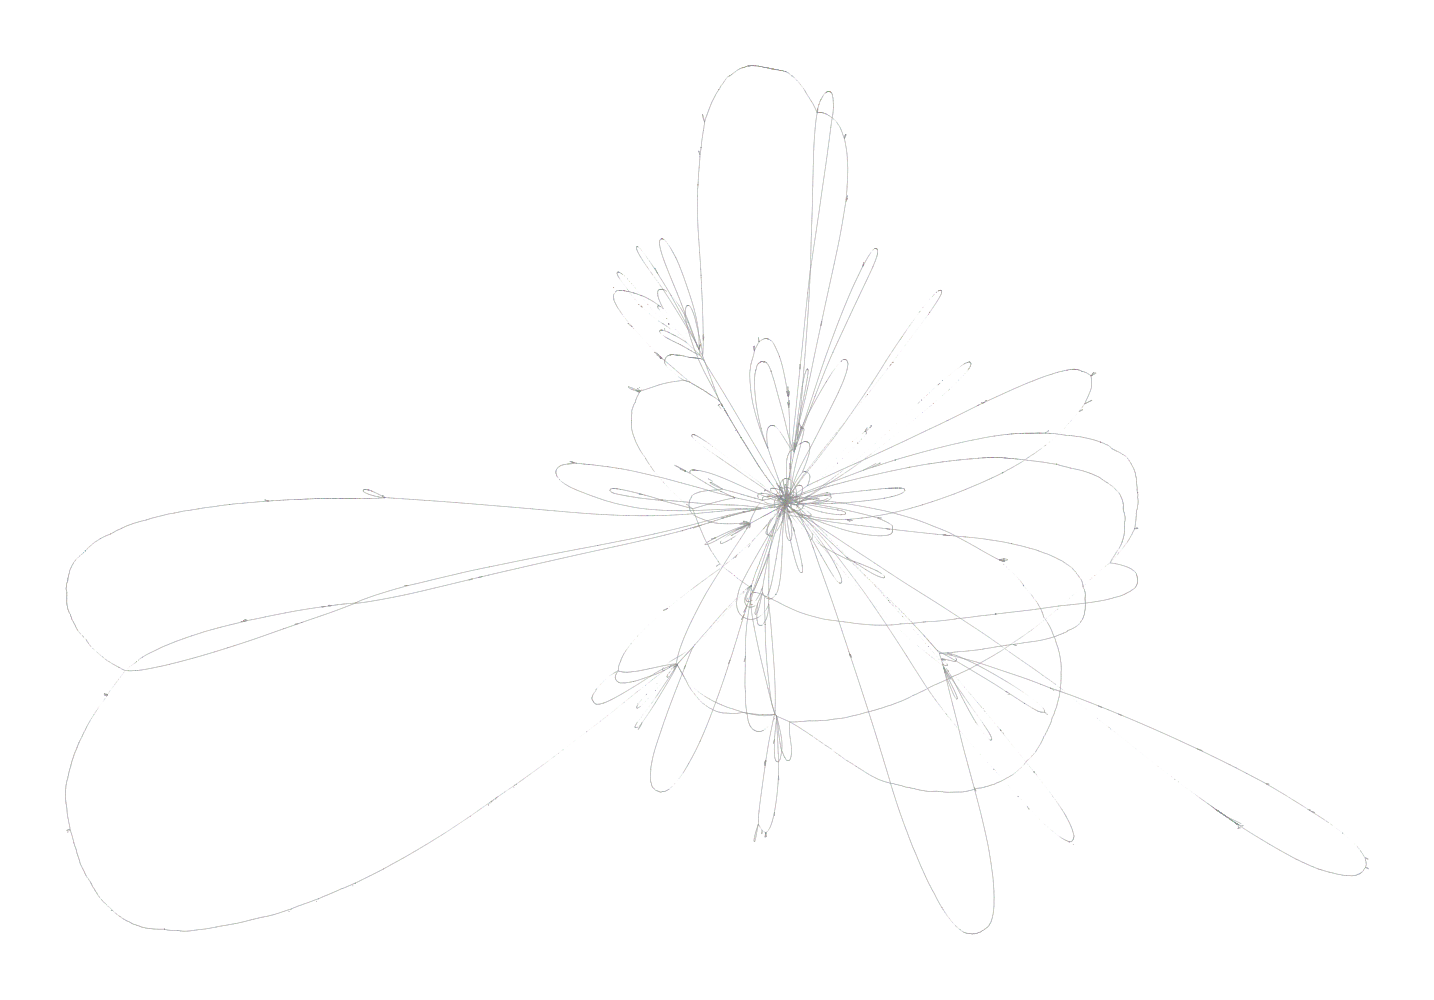
\includegraphics[width=1.0\textwidth]{Chapter3/Figs/vg_msga_yeast.png}
    \caption{{\tt vg msga} assembly} \label{subfig:msga_yeast_bandage}
  \end{subfigure}
  \caption[Whole genome alignment graphs for \emph{S. cerevisiae}]{
    Whole genome alignment graphs for \emph{S. cerevisiae} visualized using Bandage.
    The scale in \ref{subfig:msga_yeast_bandage} is greater than that in \ref{subfig:cactus_yeast_bandage}, with the latter showing a greater propensity to collapse repeat structures.
  }
  \label{fig:yeast_bandage}
\end{figure}

\subsection{Using long read mapping to evaluate \emph{cerevisiae} graphs} % from paper / my experiments
\label{sec:yeast_long_read}

In this section I evaluate the graphs I constructed in section \ref{sec:constructing_yeast_graphs} and simultaneously demonstrate the ability of {\tt vg} to align long reads to graphs of any type.
For each of the seven graphs I aligned a set of 43,337 Pacific Biosciences SK1 reads (mean length 4.7 kb) from \cite{yue2017contrasting} to the graph.
We can then compare the alignment identity for each read across the various graphs.
I do so using the same dot plot technique used to demonstrate alignment quality improvement using the Illumina data from the NCYC strains.
In figure \ref{fig:pacbio_yeast} I present a number of pairwise comparisons based on this read set.

I find that the SGD\_2010 reference provides a better match for the SK1 PacBio reads than the S288c assembly (top left), which can be seen in a subset of reads that map nearly perfectly to the SGD\_2010 graph but not to the S288c one.
This may be due to the higher quality and curation of the SGD reference, which was initially based on BACs and capillary sequencing, but I have not determined the exact cause of this discrepancy.
This same effect is clear in the comparison of S288c and the SGRP2 (top middle, figure \ref{fig:pacbio_yeast}), although there the SNPs in the SGRP2 graph tend to improve the overall match between the SK1 reads and the graph, which can be seen in a shift in density upwards from the diagonal.
For other comparisons I focused on using the S288c reference, as it forms a part of the progressive alignments and the source data for the minia assemblies comes from the same paper.

The minia graphs appear to provide very low quality as a reference for the alignment of long reads (bottom left and middle, figure \ref{fig:pacbio_yeast}).
The minia unitig graph is too fragmented for any practical use.
In almost no case does it provide a better match for the long reads.
However, while the minia contig graph is also outperformed by the S288c graph, for a notable subset of the reads it provides a perfect match, while the S288c graph fails to match them at all.
This suggests that some contigs in the Illumina assembly match the SK1 strain, which is to be expected and demonstrates that in principle this kind of graph can represent multiple genomes.

Finally, the whole genome alignment graphs are notable in their similarity.
Despite the fact that they were constructed using different algorithms, both provide a similar basis for alignment of the SK1 reads.
It is notable that alignment time against the {\tt vg msga} graph was the highest of the tested graphs, and significantly higher than that for the Cactus graph.
This may relate to the un-collapsed state of the repeats in the graph.
The alignment algorithm will attempt more alignments for each band where there is ambiguity, and the ``patching'' at the end of the alignment process will be more intensive.

\begin{figure}[htbp!]
  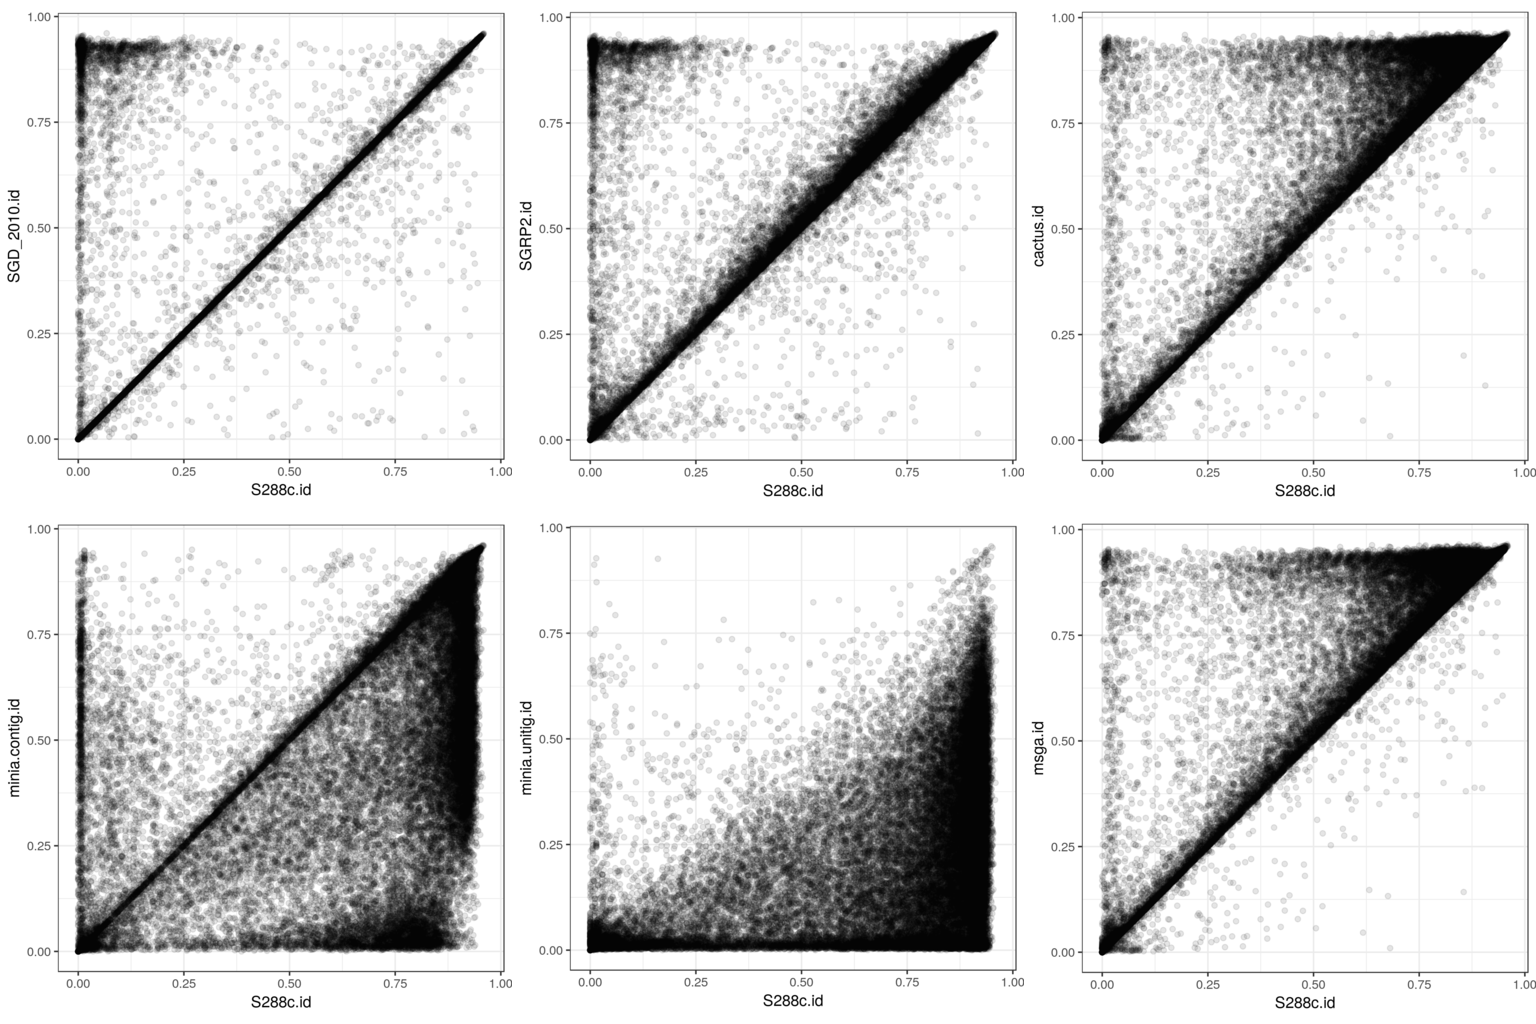
\includegraphics[width=1.0\textwidth]{Chapter3/Figs/montage_vs_S288c_3x2.png}
  \caption[Long read alignment against various \emph{S. cerevisiae} pangenome graphs]{Density plots of alignment identity when mapping 43,337 Pacific Biosciences long reads from the SK1 strain to different variation graphs.
    \emph{Linear assemblies}:
    (Top left) the SGD\_2010 reference vs. the S288c assembly from \cite{yue2017contrasting}.
    (Top middle) the S288c assembly vs. the SGRP2 SNP pangenome.
    \emph{Assembly graphs from Illumina data}:
    (Bottom left) the minia contig graph vs. the S288c assembly.
    (Bottom middle) the minia unitig graph vs. the S288c assembly.
    \emph{Whole genome alignment graphs}:
    (Top right) the Cactus alignment vs. the S288c assembly.
    (Bottom right) the {\tt vg msga} alignment vs. the S288c assembly.
  }
  \label{fig:pacbio_yeast}
\end{figure}


\section{Human}
%*0.5p 0.5h*

For a species such as human, with only 0.1\% nucleotide divergence on average between individual genome sequences, over 90\% of 100-bp reads will derive from sequence exactly matching the reference.
Therefore, new mappers should perform at least as well for linear reference mapping as the current standard, which we take to be {\tt bwa mem} with default parameters.
We show that vg does this, and then that vg maps more informatively around divergent sites.

\subsection{1000GP graph construction and indexing}
%*3p 3h*

The final phase of the 1000 Genomes Project (1000GP) produced a data set of ~80 million variants in 2,504 humans \cite{1000g2015}.
We made a series of vg graphs containing all variants or those above minor allele frequency thresholds of 0.1\%, 1\%, or 10\%, as well as a graph corresponding to the standard GRCh37 linear reference sequence without any variation.
The full vg graph uses 3.92 GB when serialized to disk, and contains 3.181 Gbp of sequence, which is exactly equivalent to the length of the input reference plus the length of the novel alleles in the VCF file.
Complete file sizes including indices range from 25 GB to 63 GB, with details including build and mapping times given in table \ref{table:1000GP}.

\begin{table}[h]
\begin{tabular}{l||c|cc|cc|cc}
\itshape Reference set & \itshape N vars & \multicolumn{2}{c}{\itshape vg} & \multicolumn{2}{c}{\itshape index} & \multicolumn{2}{c}{\itshape search time}\\
& \itshape (M) & \itshape time & \itshape size & \itshape time & \itshape size & \itshape  PE & \itshape SE\\
\hline
GRCh37 & 0 & 1:09:54 & 1.76 & 23:30:41 & 25.11 & 33:34 & 28:33 \\
1000GP AF0 & 84.8 & 3:42:01 & 3.92 & 51:05:07 & 63.28 & 45:10 & 39:46 \\
1000GP AF0.001 & 30.2 & 2:00:08 & 2.58 & 31:45:12 & 38.10 & 39:33 & 32:53 \\
1000GP AF0.01 & 14.3 & 1:35:02 & 2.17 & 27:18:53 & 30.94 & 33:13 & 27:09\\
1000GP AF0.1 & 6.8 & 1:23:04 & 1.97 & 26:06:38 & 27.79 & 32:35 & 28:43 \\
\hline
\end{tabular}
\caption[1000GP variation graphs]{Numbers of variants, file sizes in gigabytes (GB) and build and search times in hours:minutes:seconds for various human vg graphs and associated indexes. Reference sets are the linear reference GRCh37, the full 1000 Genomes Project set 1000GP AF0, and subsets of 1000GP AF0 including only variants with allele frequency above thresholds 0.001 (0.1\%), 0.01 (1\%) and 0.1 (10\%) respectively.  The number of variants in millions for each of these data sets is shown.  Search times are for 10 million 150+150bp read pairs simulated from NA24385.
    Reprinted from \cite{garrison2018variation}.
}
\label{table:1000GP}
\end{table}

\subsection{Simulations based on phased HG002}
\label{sec:1000GP_sim}

We next aligned ten million 150-bp paired-end reads simulated with errors from the parentally phased haplotypes of an Ashkenazim male NA24385, sequenced by the Genome in a Bottle (GIAB) Consortium \cite{zook2016extensive} and not included in the 1000GP sample set, to each of these graphs as well as to the linear reference using {\tt bwa mem}.
Figure \ref{fig:HG002_1000GP_sim} shows the accuracy of these alignments compared with {\tt bwa mem} for the full range of frequency thresholded graphs, in terms of receiver operating characteristic (ROC) curves.

Reads that come from parts of the sequence without differences from the reference (middle panels of Figure \ref{fig:HG002_1000GP_sim}) mapped slightly better to the reference sequence (green) than to the 1000GP graph (red), which we attribute to a combination of the increase in options for alternative places to map reads provided by the variation graph, and the fact that we needed to prune some search index $k$-mers in the most complex regions of the graph.
The best balance of performance appears at the threshold of 0.01.
As expected, this difference increased as the allele frequency threshold was lowered and more variants were included in the graph.

For reads that were simulated from segments containing non-reference alleles (~10\% of reads), which are the reads relevant to variant calling, {\tt vg} mapping to the 1000GP graph (red) gave better performance than either {\tt vg} (green) or {\tt bwa mem} (blue) mapping to the linear reference (right panels of Figure \ref{fig:HG002_1000GP_sim}), because many variants present in NA24385 are already represented in the 1000GP graph.
This is particularly clear for single-end mapping, since many paired-end reads are rescued by the mate read mapping.
Overall, vg performed at least as well as bwa mem, even on reference-derived reads, and substantially better on reads containing non-reference variants.

\begin{figure}[htbp!] 
\centering    
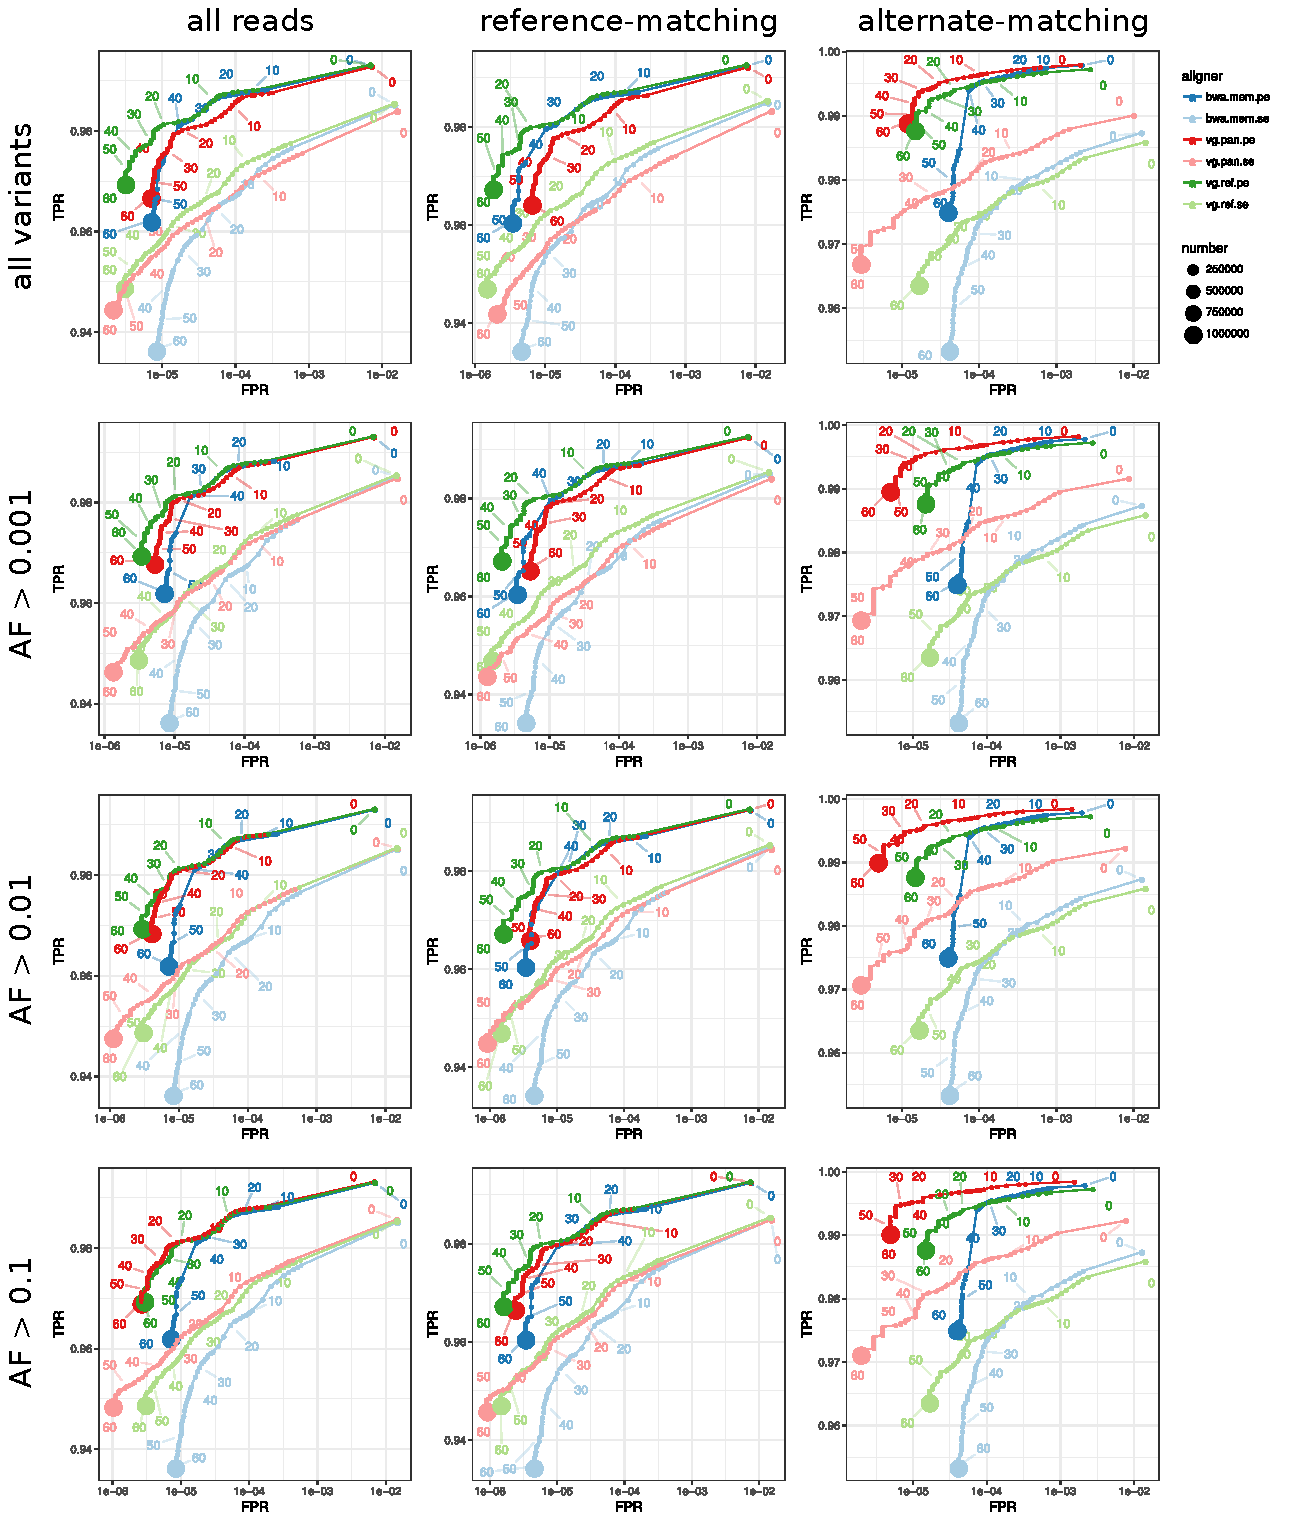
\includegraphics[width=1.0\textwidth]{Chapter3/Figs/human-10M-results-7358a67_merge_panel_labeled.pdf}
\caption[Simulated reads from HG002 versus various human pangenome graphs.]{
  ROC curves parameterized by mapping quality for 10M read pairs simulated from NA24385 as mapped by bwa mem, vg to various 1000GP pangenome references, and vg with a linear reference, using single end (se) or paired end (pe) mapping.
  Allele frequency thresholds for the various panels are (top) all variants, (second) 0.001, (third) 0.01, and (bottom) 0.1.
  Within each panel, the left subpanel is based on all reads, middle on reads simulated from segments with no genetic variants from the linear reference, right on reads simulated from segments containing variants.
  All reads may contain simulated sequencing errors reflecting SNPs at a rate of 0.01 per base and indels at a rate of 0.002 per base.
  Reprinted from \cite{garrison2018variation}.}
\label{fig:HG002_1000GP_sim}
\end{figure}

\subsection{Aligning and analyzing a real genome}

We also mapped a real human genome read set with ~50× coverage of Illumina 150-bp paired-end reads from the NA24385 sample to the 1000GP graph. vg produced mappings for 98.7\% of the reads, 88.7\%
with reported mapping quality score 30 on the Phred scale, and 76.8\% with perfect, full-length sequence identity to the reported path on the graph.
For comparison, we also used vg to map these reads to the linear reference.
Similar proportions of reads mapped (98.7\%) and with reported quality score 30 (88.8\%), but considerably fewer with perfect identity (67.6\%).
Markedly different mappings were found for 1.0\% of reads (0.9\% mapping to widely separated positions on the two graphs, and 0.1\% mapping to one graph but not the other).
The reads mapping to widely separated positions were strongly enriched for repetitive DNA. For example, the linear reference mappings for 27.5\% of these read pairs overlapped various types of satellite DNA identified by RepeatMasker, compared to 3.0\% of all read pairs.

To illustrate the consequences of mapping to a reference graph rather than a linear reference, we stratified the sites independently called as heterozygous in NA24385 by deletion or insertion length (0 for single-nucleotide variants) and by whether the site was present in 1000GP, and measured the fraction of reads mapped to the alternate allele for each category.
The results show that mapping with vg to the population graph when the variant was present in 1000GP (95.4\% of sites) gave nearly balanced coverage of alternate and reference alleles independent of variant size, whereas mapping to the linear reference either with {\tt vg} or {\tt bwa mem} led to a progressively increasing bias with increasing deletion and (especially) insertion length (Figure \ref{fig:HG002_indels}), so that for insertions around 30 bp, a majority of insertions containing reads were missing (there were over twice as many reference reads as alternate reads).

\begin{figure}[htbp!] 
\centering    
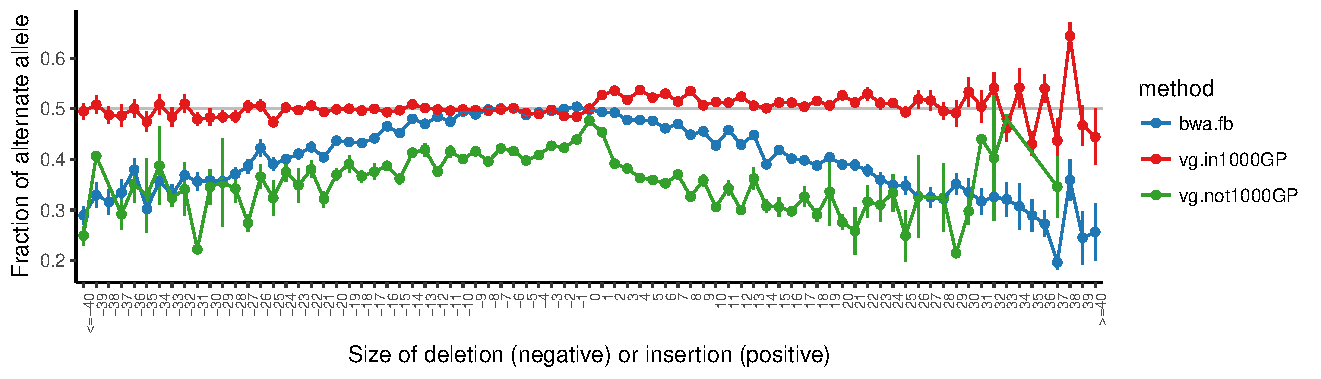
\includegraphics[width=1.0\textwidth]{Chapter3/Figs/HG002_wg_pan_ref_bwa_true_hets_allele_balance_tsv_gz_3.pdf}
\caption[Indel allele balance in HG002]{The mean alternate allele fraction at heterozygous variants previously called in HG002/NA24385 as a function of deletion or insertion size (SNPs at 0). Error bars are ± 1 s.e.m.
  Reprinted from \cite{garrison2018variation}.}
\label{fig:HG002_indels}
\end{figure}

\subsection{Whole genome variant calling experiments}

During the development phase of {\tt vg}, we explored its application to whole genome alignment and variant calling in the PrecisionFDA Truth Challenge, in which the team which developed the Genome in a Bottle truth set developed and held out a new sample.
Methods were first tested against publicly available truth sets on NA12878 in the ``consistency'' challenge, in which the {\tt vg} development team received a star for ``heroic effort'' in completing the first whole-genome graph based alignment and variant calling analysis.
The results for this first iteration were very poor, with F-scores for indels and SNPs around 95\%.
The computational costs were high, with the run consuming around \$1000 in resources on Amazon's Elastic Compute cloud (AWS EC2).

In the final round of the challenge, we obtained results as described in table \ref{table:PFDA}.
We find that the {\tt vg} pipeline had similar performance to the \emph{de novo} assembly pipeline fermikit for SNPs.
Methods that are not explicitly based on the GATK indel calling method perform notably worse on indels, including egarrison-hhga\footnote{This was my work along with Nicolas Della Penna, \url{https://github.com/ekg/hhga}. Unfortunately, it remains unpublished.}, which used Platypus, fermikit, and freebayes to generate candidate variants and implemented a genotyper using a machine learning method, and mlin-fermikit, which was a direct application of fermikit's standard pipeline to the data for HG002.
However, {\tt vg call}'s indel calling results were very poor, and likely caused by bugs in the variant caller and aligner at this stage rather than conceptual problems with graph based variant calling.

\begin{table}[h]
\begin{tabular}{l||ccc|ccc}
\itshape Submission & \multicolumn{3}{c}{\itshape SNPs} & \multicolumn{3}{c}{\itshape indels}\\
& \itshape F-score & \itshape recall & \itshape precision & \itshape F-score & \itshape recall & \itshape precision \\
\hline
anovak-vg & 98.4545 & 98.3357 & 98.5736 & 70.4960 & 69.7491 & 71.2591 \\
astatham-gatk & 99.5934 & 99.2091 & 99.9807 & 99.3424 & 99.2404 & 99.4446 \\
bgallagher-sentieon & 99.9296 & 99.9673 & 99.8919 & 99.2678 & 99.2143 & 99.3213 \\
dgrover-gatk & 99.9456 & 99.9631 & 99.9282 & 99.4009 & 99.3458 & 99.4561 \\
egarrison-hhga & 99.8985 & 99.8365 & 99.9607 & 97.4253 & 97.1646 & 97.6874 \\
hfeng-pmm3 & 99.9548 & 99.9339 & 99.9756 & 99.3628 & 99.0161 & 99.7120 \\
mlin-fermikit & 98.8629 & 98.2311 & 99.5029 & 95.5997 & 94.8918 & 96.3183 \\
rpoplin-dv42 & 99.9587 & 99.9447 & 99.9728 & 98.9802 & 98.7882 & 99.1728 \\
\hline
\end{tabular}
\caption[Selected results from the PrecisionFDA Truth Challenge]{A selected subset of PrecisionFDA Truth Challenge results showing the best-performing methods as well as a number of other notable submissions.}
\label{table:PFDA}
\end{table}

We also explored integration of vg with the recently published GraphTyper \cite{eggertsson2017graphtyper} method, which calls genotypes by remapping reads to a local, partially ordered variation graph built from a VCF file, relying on initial global assignment to a region of the genome by mapping with bwa to a linear reference.
Therefore, although GraphTyper also scales to the whole human genome because it is essentially a local method, its functionality is complementary to that of vg, which maps to a global variation graph and does not directly call genotypes.
In experiments where we used vg rather than bwa as the primary mapper for GraphTyper, true positives increased marginally (0.02\% for single-nucleotide polymorphisms (SNPs) and 0.06\% for indels) while false positives increased for SNPs by 0.15\% and decreased for indels by 0.03\%.
We note, however, that GraphTyper was developed by its authors for {\tt bwa mem} mapping.

\subsection{A graph of structural variation in humans}
%*2.5p 5h*

The Human Genome Structural Variation Consortium (HGSVC)\footnote{\url{http://www.internationalgenome.org/human-genome-structural-variation-consortium/}} has continued the difficult process of cataloging structural variation in humans.
Recently, the group has developed a set of haplotype-resolved structural variation callsets for six individuals \cite{chaisson2018multi}.
These variant calls are derived from many sources, and are unified into a common framework in phased VCF files.
I built a graph from these variants and the GRCh38 reference against which they are represented, then used {\tt vg map} to align short reads from a sample in the HGSVC set (NA19240) as well as a sample that was not included (HG002/NA24385).

Although I mapped only 1M read pairs, alignments to the HGSVC graph were significantly better (when measured via the identity metric) than alignments to the GRCh38 linear reference (figure \ref{fig:hgsvc_alignment}).
This was much more significant in the case of NA19240 (two sample T-test $p$-value = 0.008529) than for NA24385 ($p$-value = 0.06813).
Presumably the lower number of shared alleles with NA24385 means a larger set of reads would need to be mapped to obtain a clear result.
The HGSVC graph did not significantly improve alignment scores for 1M random reads (only 2.4\% align, with $p$-value = 0.9889), or for reads sampled without error ($p$-value = 0.4665) or with 0.5\% SNP error and 0.1\% indel error from GRCh38 ($p$-value = 0.9106).

These results are statistically significant and our negative controls validate that the representation in the reference of recurrent SV polymorphisms contributes to the improvement in alignment performance.
However, it would be most interesting to see that the variant calling process implemented in {\tt vg call} could genotype the structural variants in these samples.
Investigations into this are ongoing, and although the results are promising they are not yet complete.
As the HGSVC graph is produced from SV calls in a VCF, we retain the original problems of representing structural variation in VCF.
We cannot represent nested variation, and so alleles that are only marginally different are represented as completely separate paths in the resulting graph.
This adds ambiguity to the mapping and apparently causes problems when attempting to use the graph for variant calling.

\begin{figure}[htbp!] 
  \centering
  \begin{subfigure}[t]{0.49\textwidth}
    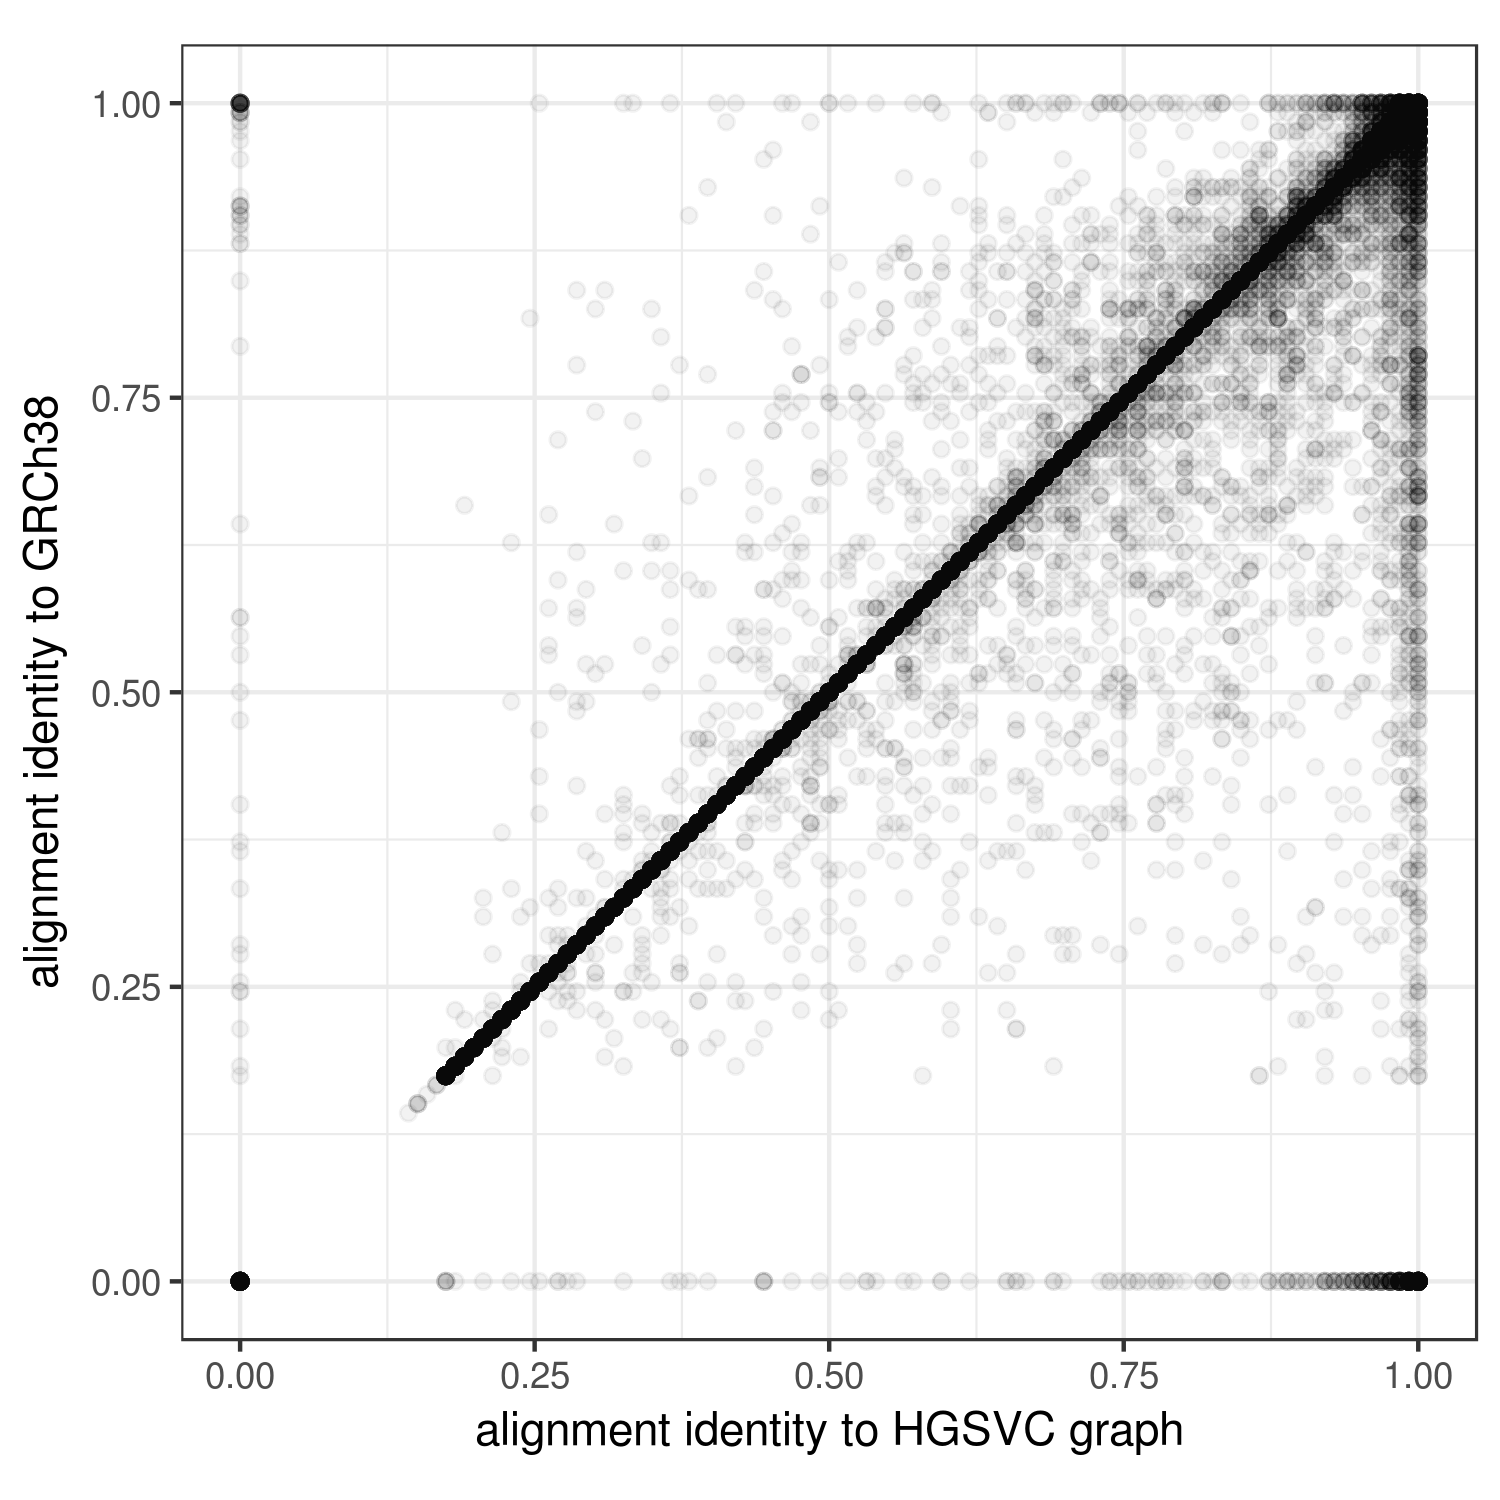
\includegraphics[width=1.0\textwidth]{Chapter3/Figs/NA19240_hg38_vs_HGSVC_scatter.png}
    \caption{NA19240 HGSVC vs. GRCh38}
    \label{subfig:hgsvc_NA19240_scatter}
  \end{subfigure}
  \begin{subfigure}[t]{0.49\textwidth}
    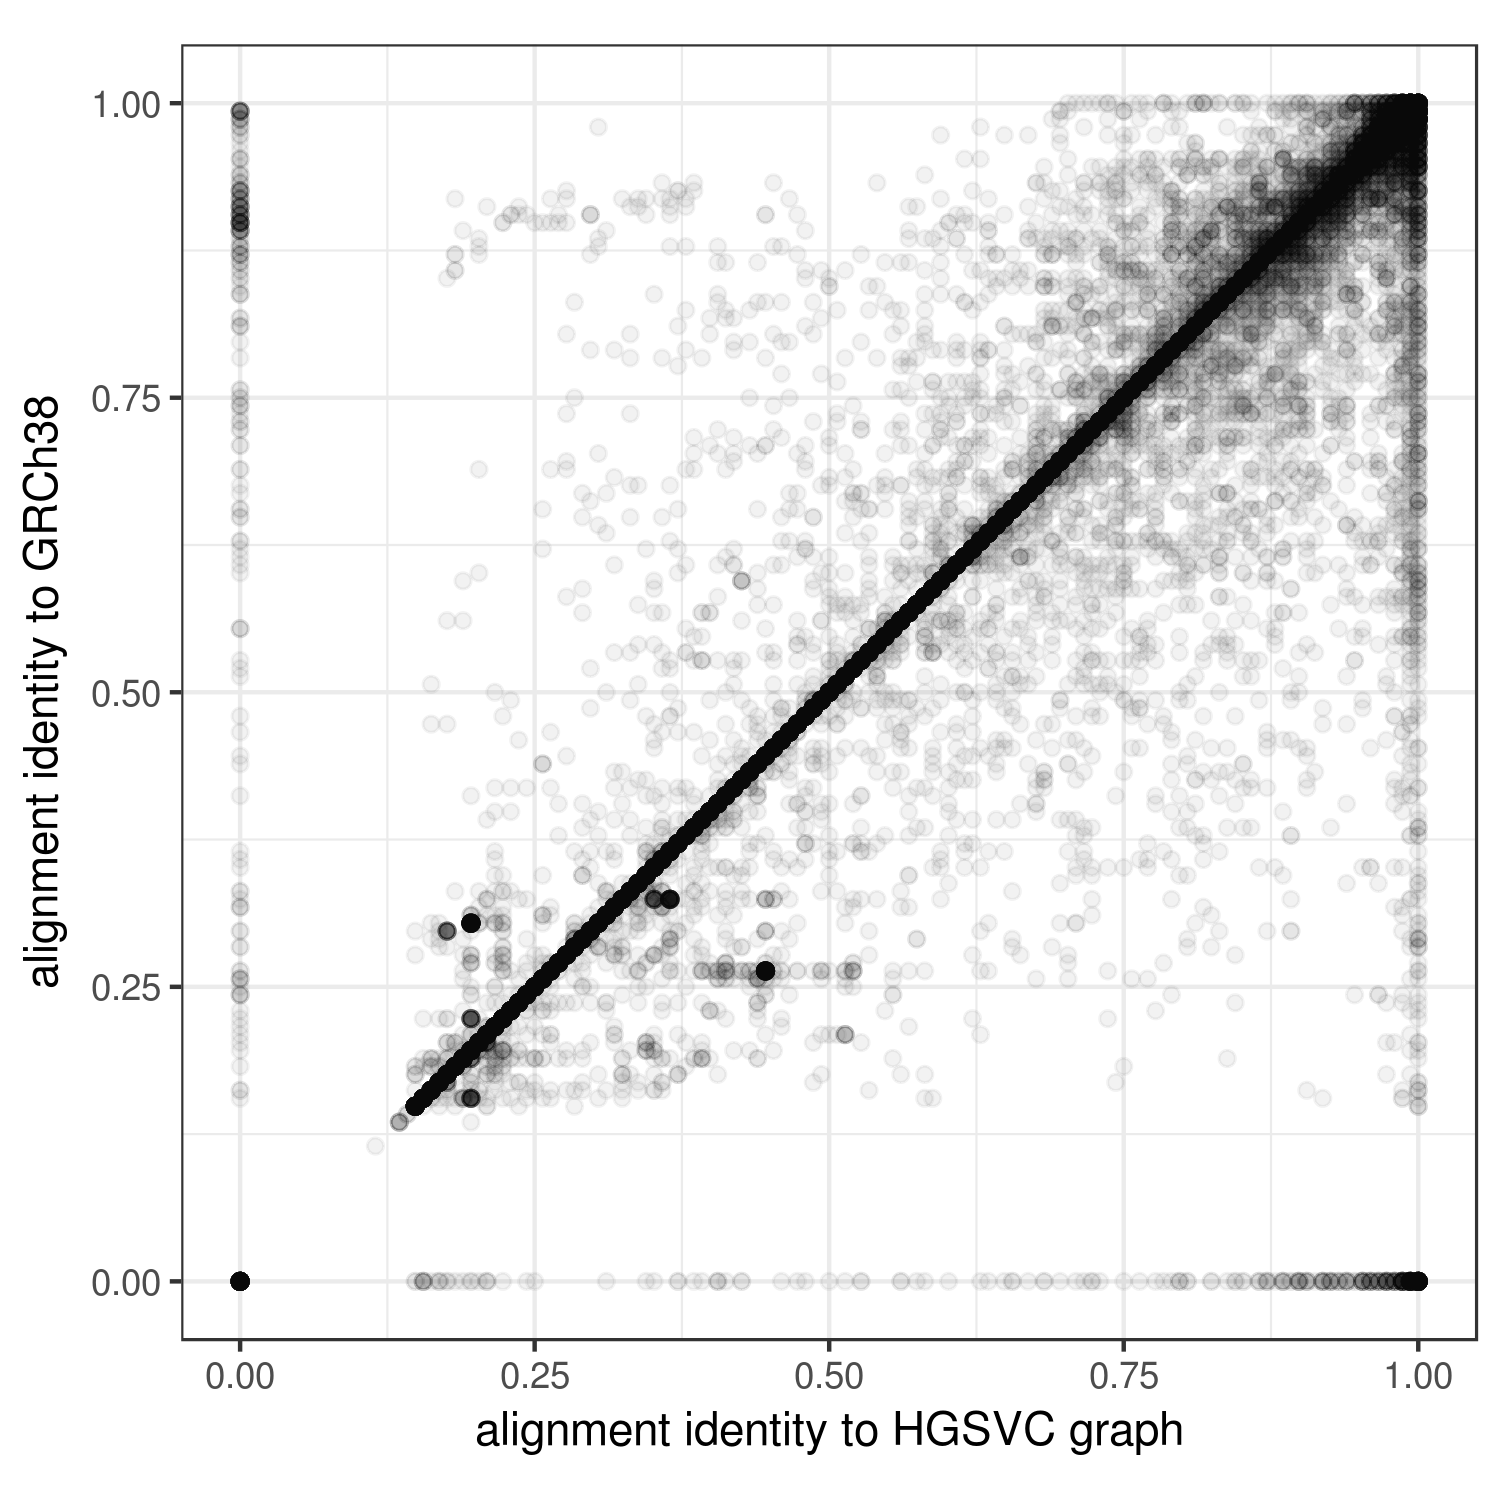
\includegraphics[width=1.0\textwidth]{Chapter3/Figs/NA24385_hg38_vs_HGSVC_scatter.png}
    \caption{NA24385 HGSVC vs. GRCh38}
    \label{subfig:hgsvc_NA24385_scatter}
  \end{subfigure}
  \begin{subfigure}[t]{0.49\textwidth}
    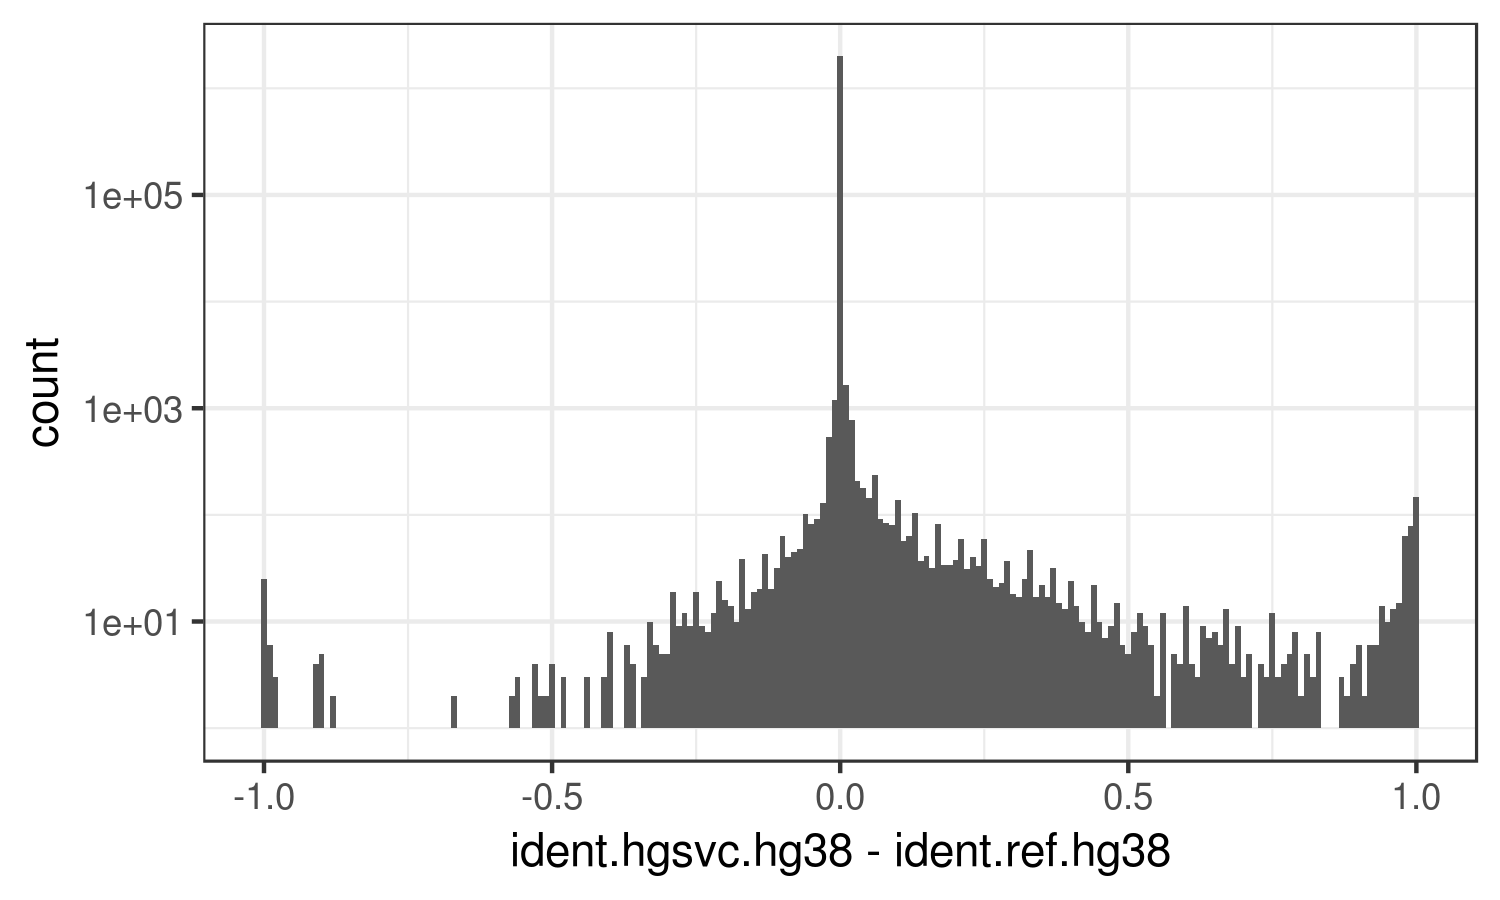
\includegraphics[width=1.0\textwidth]{Chapter3/Figs/NA19240_hg38_vs_HGSVC_hist.png}
    \caption{NA19240 HGSVC - GRCh38}
    \label{subfig:hgsvc_NA19240_hist}
  \end{subfigure}
  \begin{subfigure}[t]{0.49\textwidth}
    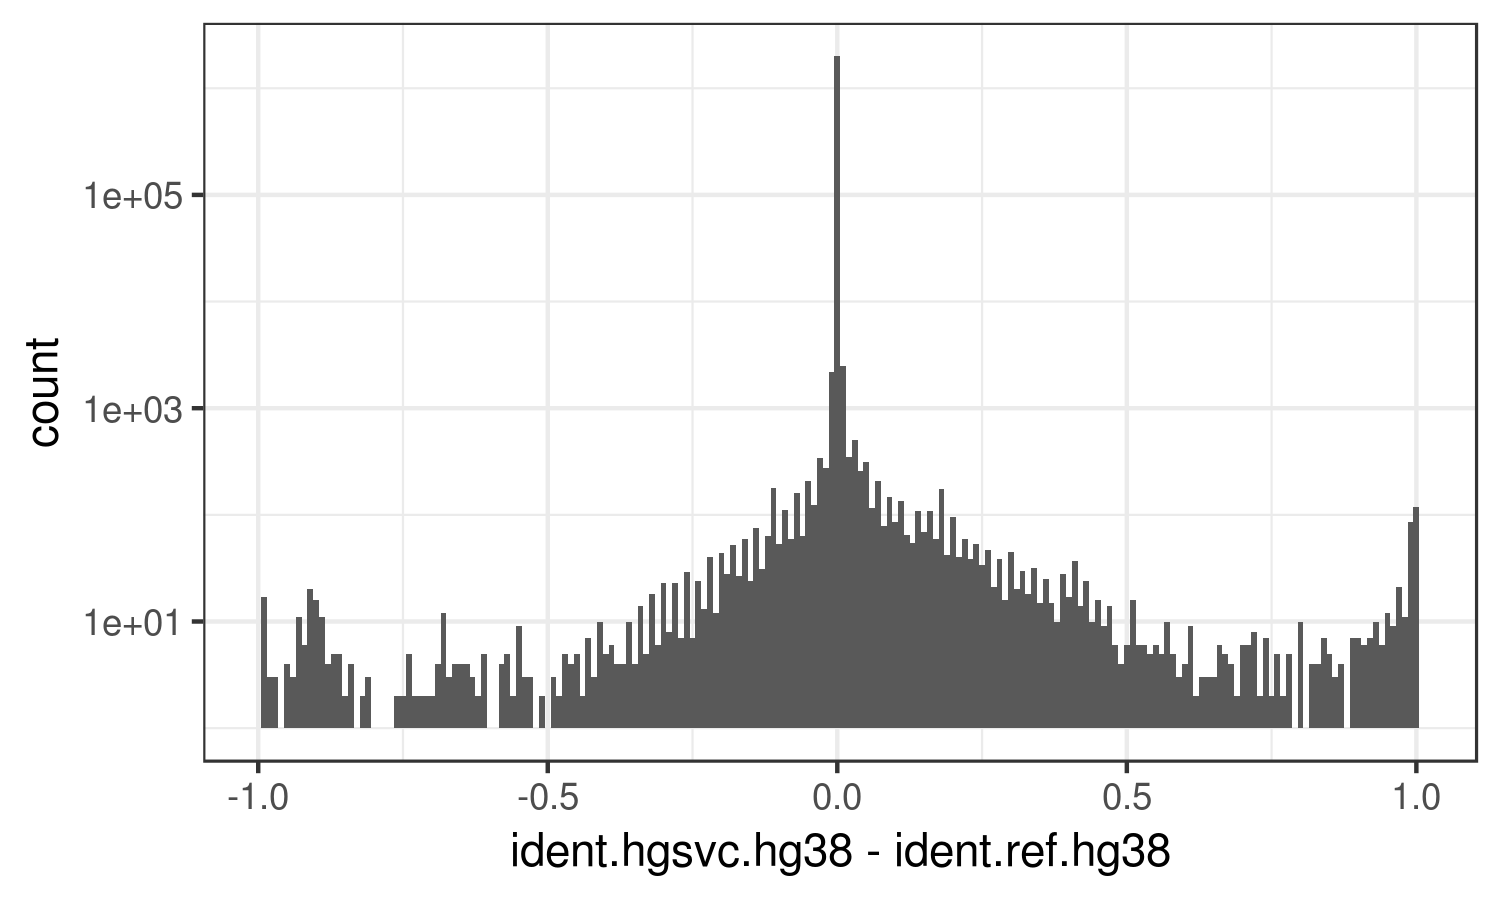
\includegraphics[width=1.0\textwidth]{Chapter3/Figs/NA24385_hg38_vs_HGSVC_hist.png}
    \caption{NA24385 HGSVC - GRCh38}
    \label{subfig:hgsvc_NA24385_hist}
  \end{subfigure}
  \caption[Alignment against the HGSVC graph]{
    1M 2x150bp Illumina read pairs from NA19240 (which is in the HGSVC graph) and NA24385/HG002, which is not, aligned against both the HGSVC graph and the GRCh38 reference, then compared.
    In panels \ref{subfig:hgsvc_NA19240_scatter} and \ref{subfig:hgsvc_NA24385_scatter} the difference in performance is seen by the alignments which have positive identity against the HGSVC graph but 0 identity against the GRCh38 reference.
    Panels \ref{subfig:hgsvc_NA19240_hist} and \ref{subfig:hgsvc_NA24385_hist} are log-scaled histograms of the difference in alignment score.
    In these we can observe a small subset of reads which map to the HGSVC graph but not GRCh38 as increased density at 1.0.
   }
\label{fig:hgsvc_alignment}
\end{figure}


\subsection{Progressive alignment of human chromosomes}

There are only a few truly \emph{de novo} human genome assemblies which achieve near-complete chromosomes, and so a reference-guided variant detection approach has prevailed for the discovery of novel structural variation \cite{fan2017hysa}.
Using {\tt vg msga}, I explored if it would be possible to use the HGSVC reference-guided assemblies directly in progressive alignment.
It was possible to produce the progressive alignment of the six haplotypes for chr20 on system I used at the Sanger for most experiments, which has 256GB of RAM and 32 vCPUs.
However, doing so took more than week of wall clock time, suggesting that this approach is untenable in its current form.
I was not able to complete the progressive alignment of the six haplotypes of chromosome 2.
Optimization may improve the performance of {\tt vg msga}, but the linear nature of the approach suggests that aligning more than a handful of sequences will never be feasible.

The progressive assembly can be seen to compress the input.
The resulting graph contains 76,875,262bp of sequence, while the input FASTA file of the six haplotypes contains 386,748,228bp, around a 5-fold compression.
This result serves to demonstrate that the hierarchical alignment process can scale to many tens of megabases.
The low performance of the method prevented its application to the whole genome.

\subsection{Building graphs from the MHC}

In \cite{novak2017genome} we explored methods to build graphs from the GRCh38's ALT sequences and reference genome.
One of the most challenging regions is the Major Histocompatibility Complex (MHC) on chromosome 6.
In this ~5Mb region, balancing selection has generated a high level of genetic diversity, and today we observe up to 40 million years of divergence between alternative copies of the locus, dating far back into the primate lineage.
Previous efforts to build reference graphs from this region have often required hand curation to achieve reliable results \cite{dilthey2015improved}.

Automatically building a sensible MHC graph with tools in {\tt vg} requires that the tools work correctly, and over the course of my work I have used this region as an important test case.
It took nearly a year for {\tt vg msga} to mature enough to build the MHC graph without crashing, and another two years before my long read alignment implementation became capable of developing a sensible result.

My further interest in the problem of building graphs from sequences yielded {\tt seqwish} (section \ref{sec:from_pairwise_alignments}).
{\tt seqwish} losslessly induces the variation graph implied by a set of sequence alignments.
It implements a disk-backed bidirectional alignment graph akin to that described in \cite{kehr2014genome}, and with a similar objective as tools developed in \cite{jandrasits2018seq}.
The goal is to build a pangenome graph in which pairwise alignments between the sequences define the graph.
Unlike {\tt vg msga}, it is fully dependent on an input alignment set, and is not progressive.

As an exposition of the differing solutions to this problem offered by these two methods, I built the MHC graph from the 9 haplotypes overlapping the MHC in GRCh38\footnote{These were collected for use in the GA4GH-DWG by the human genome variation map (HGVM) project \cite{blow2015decoding}.}.
To build the {\tt seqwish} graph, I used \cite{li2018minimap2} to generate an all versus all alignment, and induce the graph from this\footnote{{\tt minimap2 MHC.fa MHC.fa -c -X -x asm20 -t 32 >MHC.paf \&\& seqwish -s MHC.fa -a MHC.paf -b MHC.seqwish >MHC.gfa}}.
With {\tt vg msga} I supplied suitable parameters to encourage greater colliniearity in the alignment, but otherwise used defaults\footnote{{\tt vg msga -f MHC.fa -w 512 -J 16384 -b ref -D >MHC.vg}}.
{\tt seqwish} used very little memory, never more than around a gigabyte, but wrote 12GB of intermediate files to disk during graph induction.
{\tt vg msga} used several times this much RAM at peak, indicating that it will be difficult to scale its application beyond small genomic regions.
Both processes took around 2 hours to complete on the 256GB/32vCPU server I used for most of the experiments in this thesis.

\begin{figure}[htbp!]
  \begin{subfigure}[t]{0.49\textwidth}
    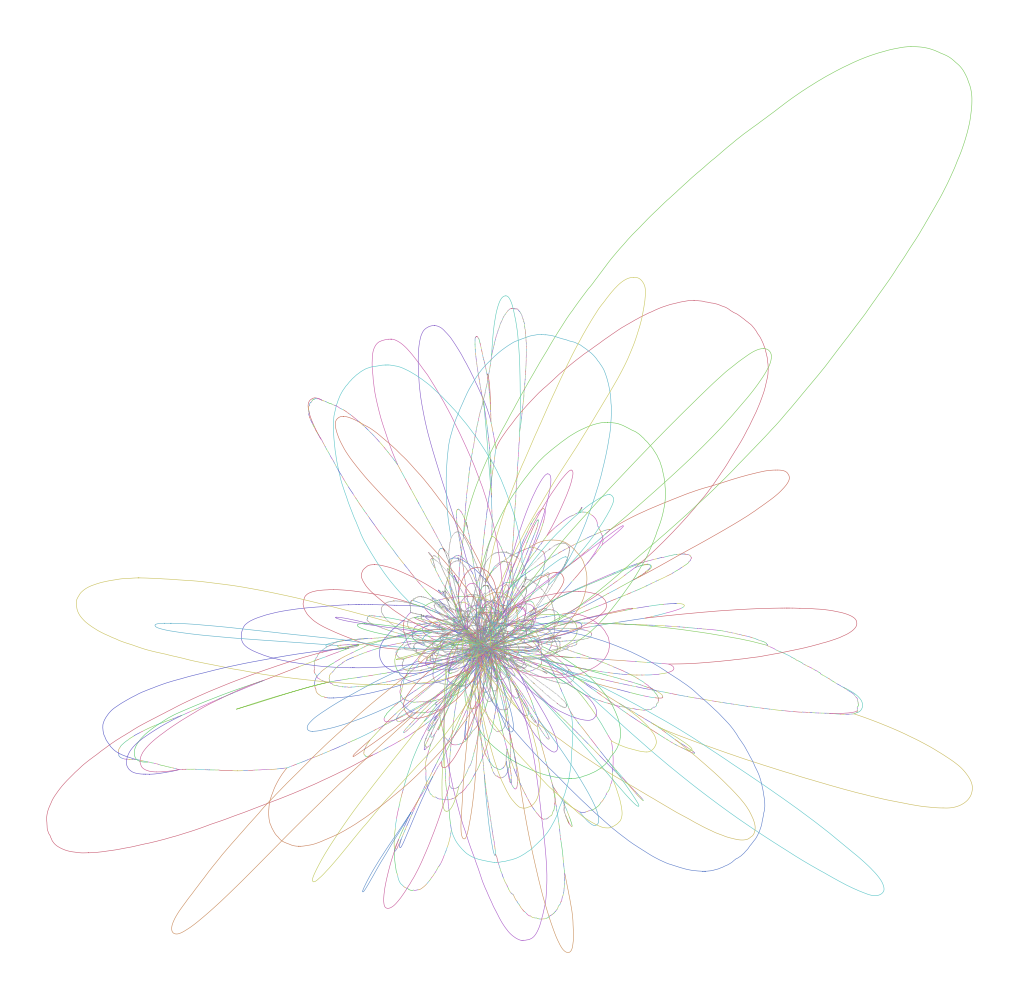
\includegraphics[width=1.0\textwidth]{Chapter3/Figs/seqwish_MHC.png}
    \caption{The full seqwish MHC graph}
    \label{subfig:seqwish_mhc_bandage}
  \end{subfigure}
  \begin{subfigure}[t]{0.49\textwidth}
    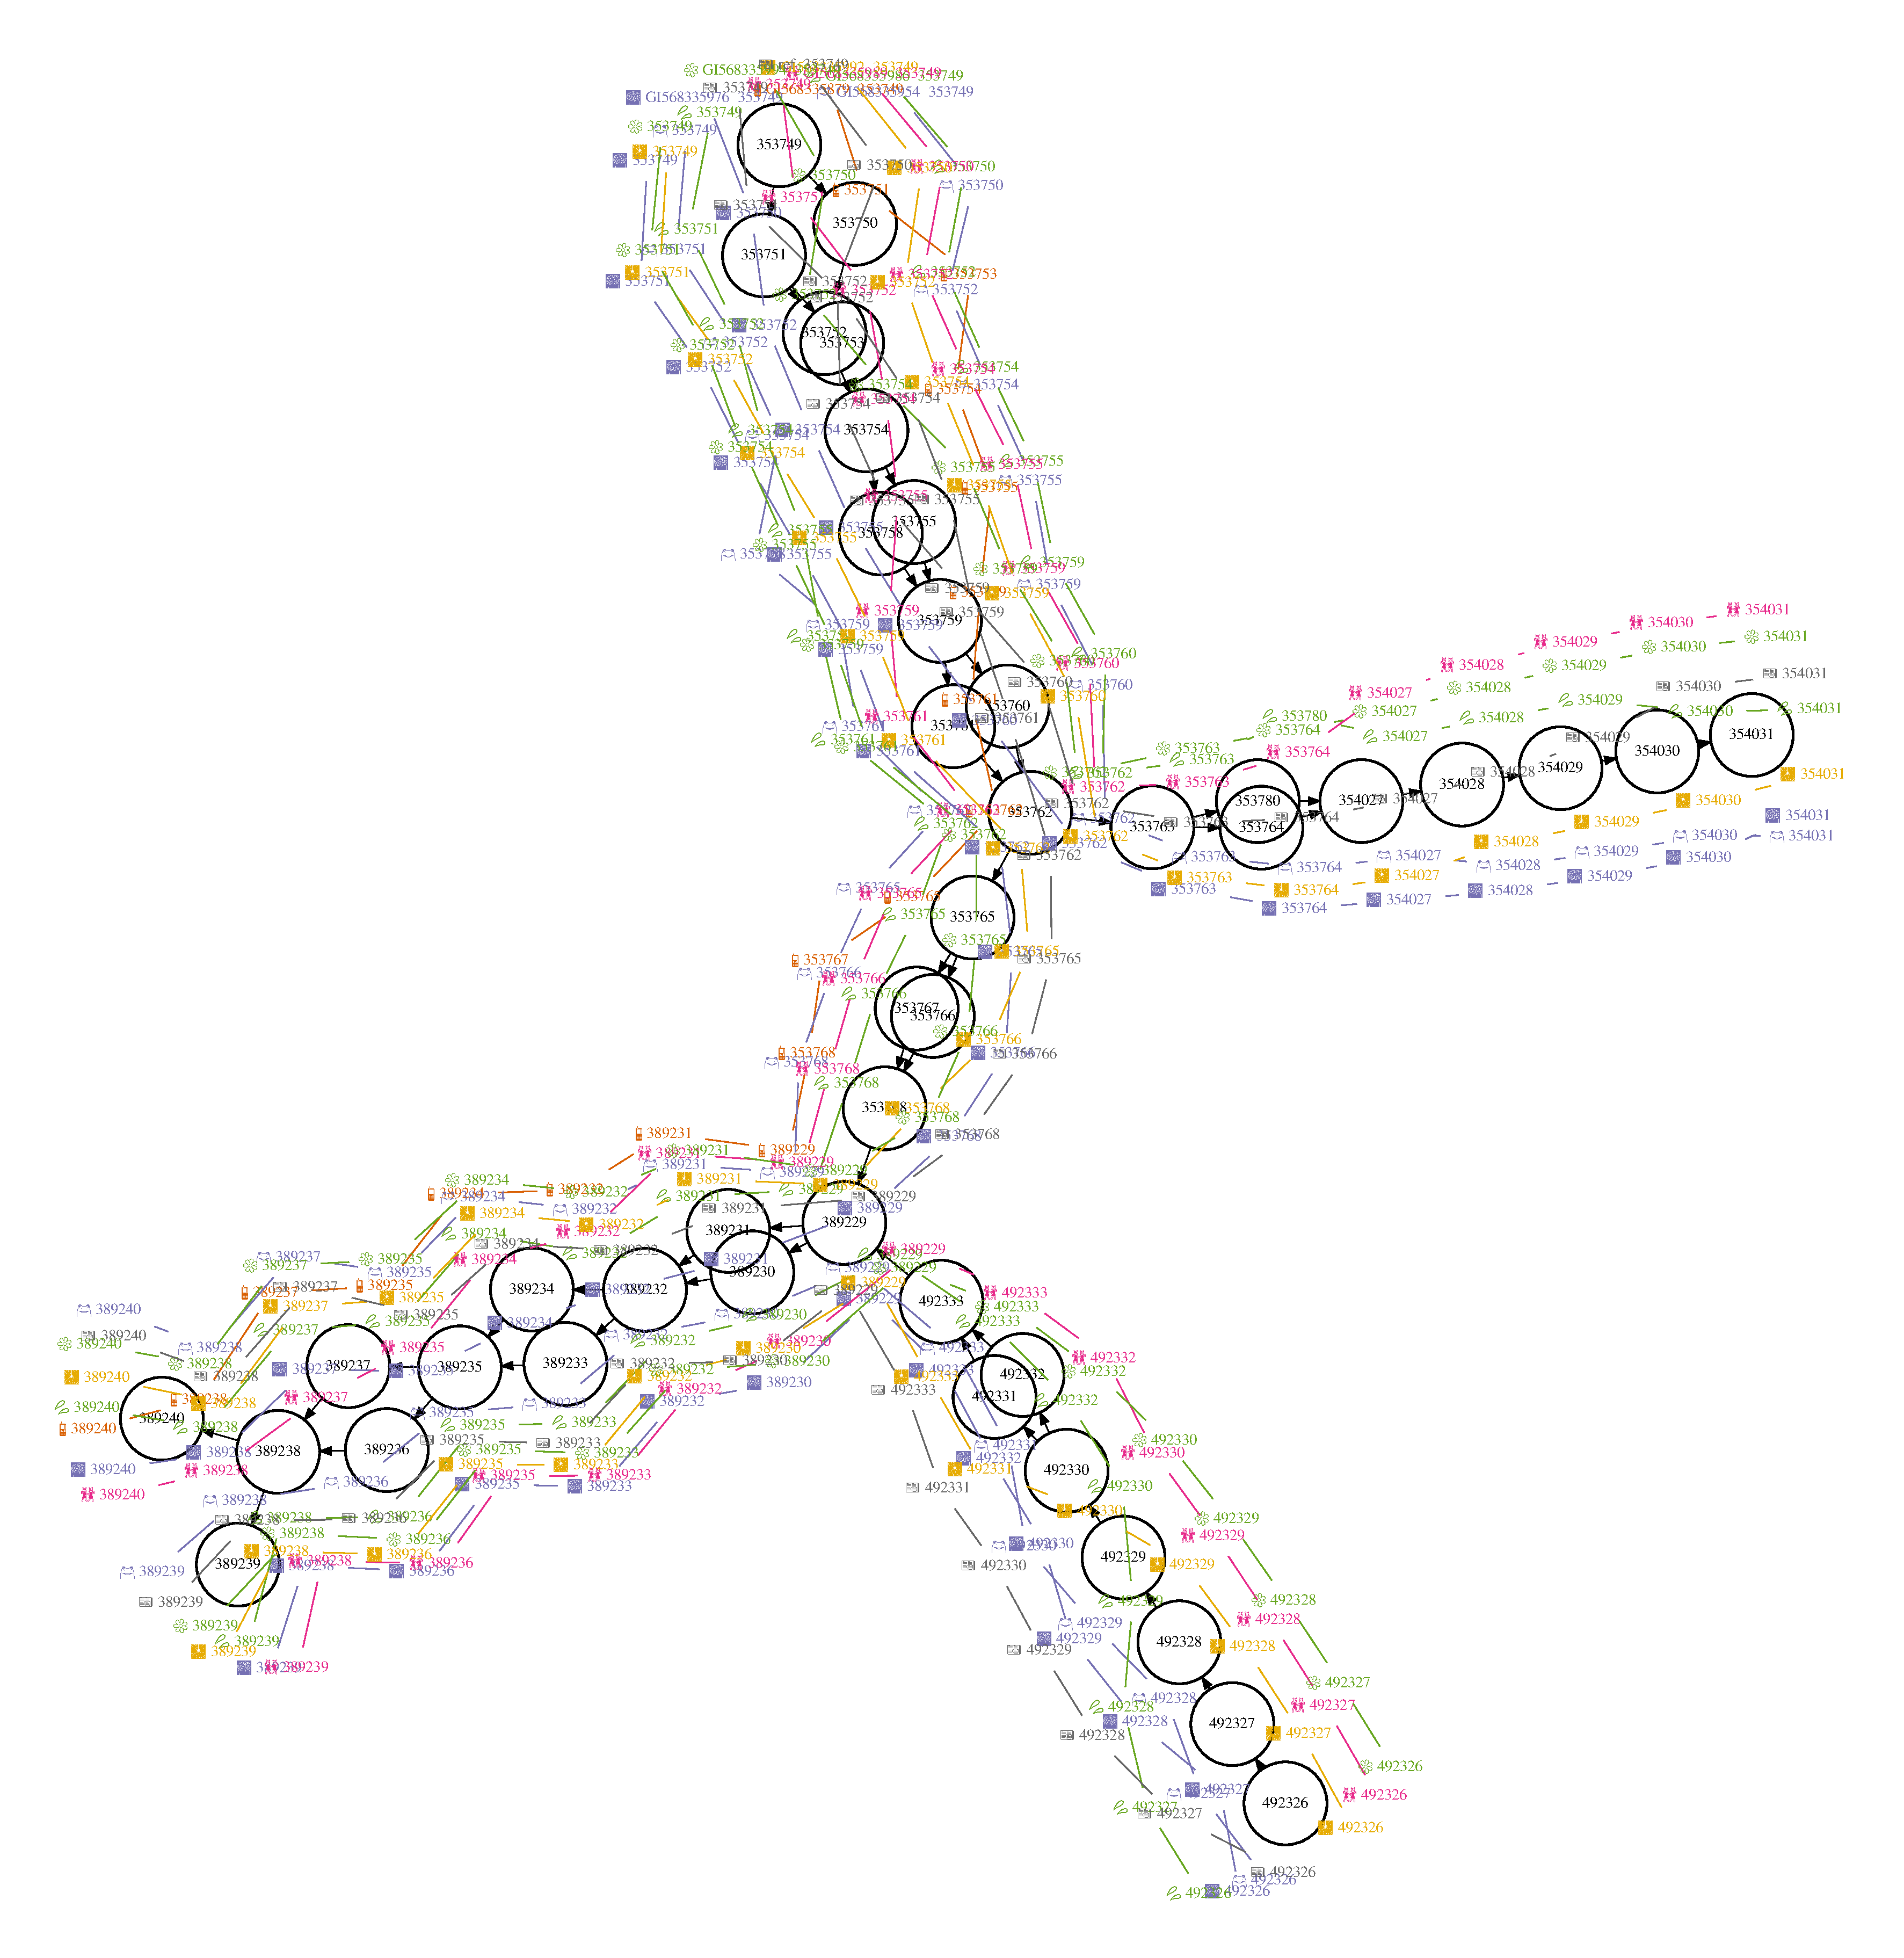
\includegraphics[width=1.0\textwidth]{Chapter3/Figs/seqwish_MHC_n353767_neato.pdf}
    \caption{A repeat in the seqwish MHC graph}
    \label{subfig:seqwish_mhc_neato}
  \end{subfigure}
  \begin{subfigure}[t]{0.9\textwidth}
    
\includegraphics[width=1.0\textwidth]{Chapter3/Figs/seqwish_MHC_n492324_viz.pdf}
    \caption{A linear component in the seqwish MHC graph}
    \label{subfig:seqwish_mhc_viz}
  \end{subfigure}
  \caption[Seqwish assembly of the MHC in GRCh38.]{
    Seqwish assembly of the MHC in GRCh38.
    In panel \ref{subfig:seqwish_mhc_bandage} Bandage was used to gain a view of the full graph.
    The fine structure of the graph is similar as for the earlier yeast assemblies.
    The core of the graph forms a hairball of repeats, as in panel \ref{subfig:seqwish_mhc_neato} flanked by low-copy loops which are locally directed and acyclic as in panel \ref{subfig:seqwish_mhc_viz}, which adjoins the subgraph plotted in panel \ref{subfig:seqwish_mhc_neato}.
  }
  \label{fig:seqwish_mhc}
\end{figure}

The {\tt seqwish} MHC graph contains 9,764,108bp of sequence, in 224,873 nodes and 321,990 edges, while the {\tt vg msga} assembly is larger, with 10,900,412bp of sequence in 480,734 nodes and 536,592 edges.
Unlike the {\tt vg msga} graph, whose nodes are cut to be shorter than 32bp to enable GCSA2 indexing during progressive construction, the seqwish graph is fully compressed by default, and this results in its much lower node count.
We can compare the aggregate results for {\tt seqwish} (figure \ref{subfig:seqwish_mhc_bandage}) to those for {\tt vg msga} (figure \ref{fig:vg_msga_mhc}).
It becomes clear from these visualizations that the {\tt seqwish} graph compresses its repeats much more than {\tt vg msga} (figure \ref{subfig:seqwish_mhc_neato}).
However, the alignment in general is sensible in that unique alignments between the input sequences generate linear components, as seen in panel \ref{subfig:seqwish_mhc_viz}.
This compression tends to confuse operations on the graph, as it reduces the distance between all positions in the graph and causes overlaps of many genomic regions in the pangenome graph.
A different parameterization of the aligner might need to be used to reconstruct the approximately nature of this genomic locus.

\begin{figure}[htbp!]
  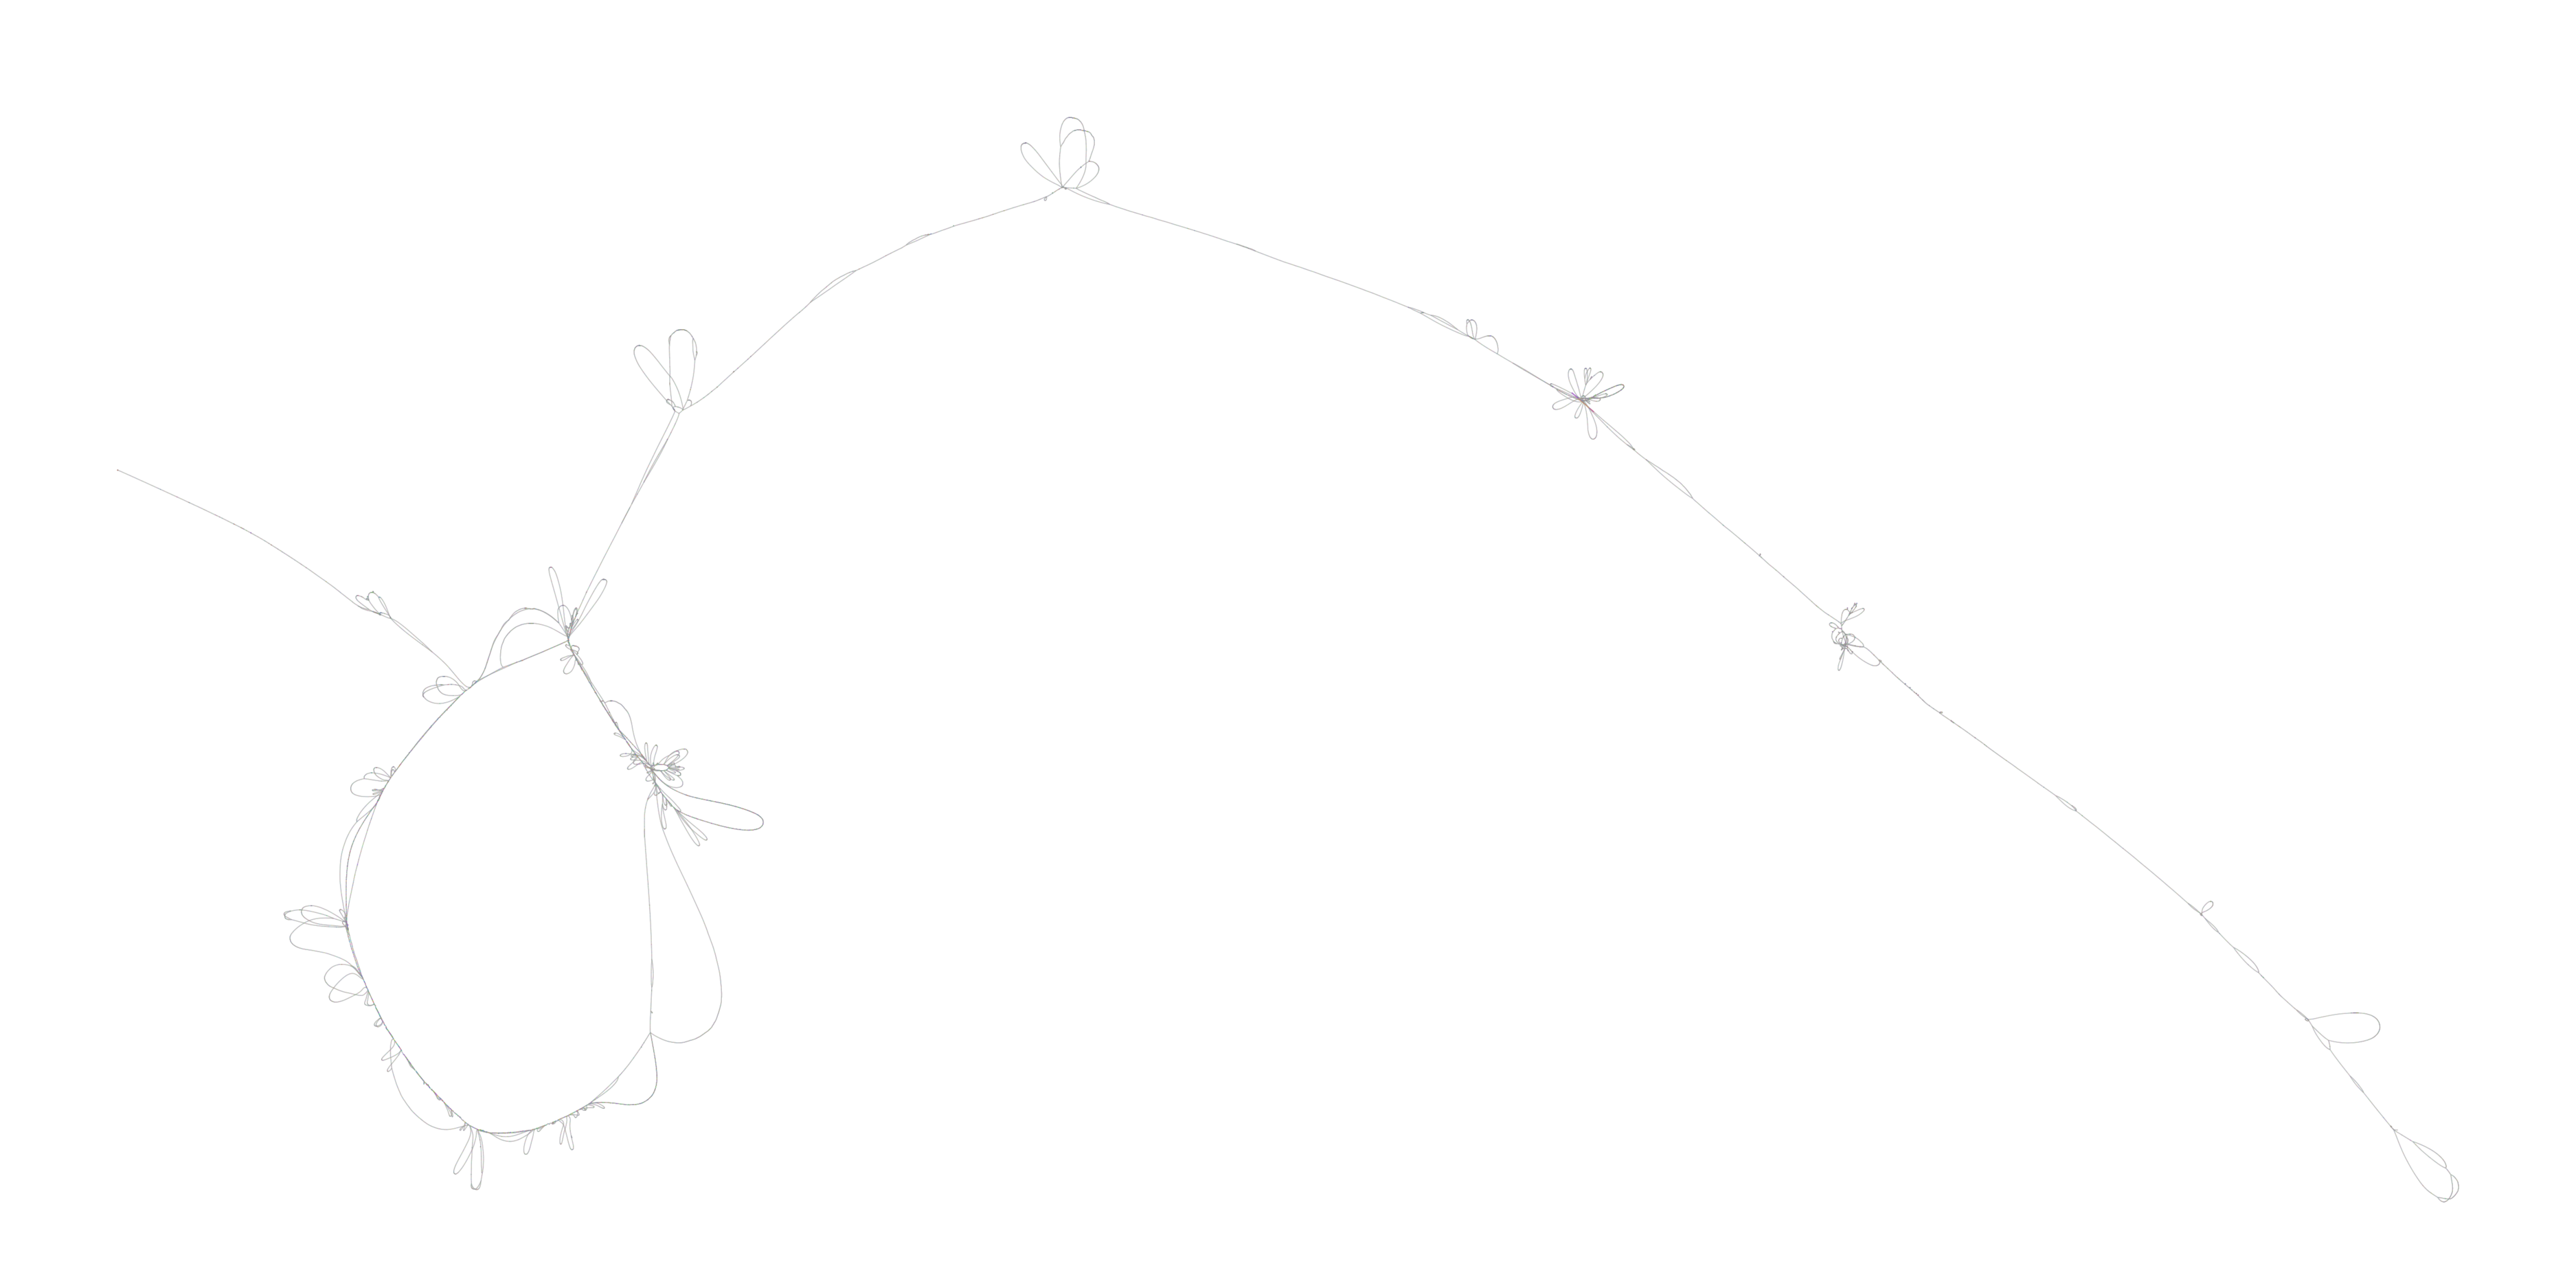
\includegraphics[width=1.0\textwidth]{Chapter3/Figs/MHC_vg-msga_v1_9_0-115-gc20e80f_gfa.png}
  \caption[{\tt vg msga} assembly of the MHC in GRCh38.]{
    {\tt vg msga} assembly of the MHC in GRCh38 as visualized by Bandage.
  }
  \label{fig:vg_msga_mhc}
\end{figure}

To appreciate the effect of repeat collapse on the resulting graph, I applied {\tt vg dotplot}, which generates dotplots from indexed variation graphs, to compare the in-graph alignments of the same pair of sequences in both the {\tt seqwish} and {\tt vg msga} graphs.
These results are presented in figure \ref{fig:mhc_dotplots}.
It is clear (in \ref{subfig:seqwish_mhc_dotplot}) that the {\tt minimap2} based alignment process encorages the collapse of repeats, which results in the large off-diagonal blocks of graph positional matches between the sequences.
In contrast, (panel \ref{subfig:vg_msga_mhc_dotplot}) shows that the sequences can naturally align through the graph in an approximately linear fashion, with little repeat collapse.
This linearity is enforced by setting a high alignment chain model ``bandwidth'' parameter ({\tt -J 16384}) (described in section \ref{sec:chunked_alignment}), which limits the size of an insertion or deletion that can be tolerated in collinear chaining.
With a primary alignment chunk size of 512 and overlap of 64, this yields an alignment chain model bandwidth of approximately 6Mb, which roughly covers the entire MHC for any input sequence.
Setting a shorter bandwidth allows repeat collapse to occur in a manner similar to what occurs when inducing the graph from the {\tt minimap2} alignments.

\begin{figure}[htbp!]
  \begin{subfigure}[t]{0.49\textwidth}
    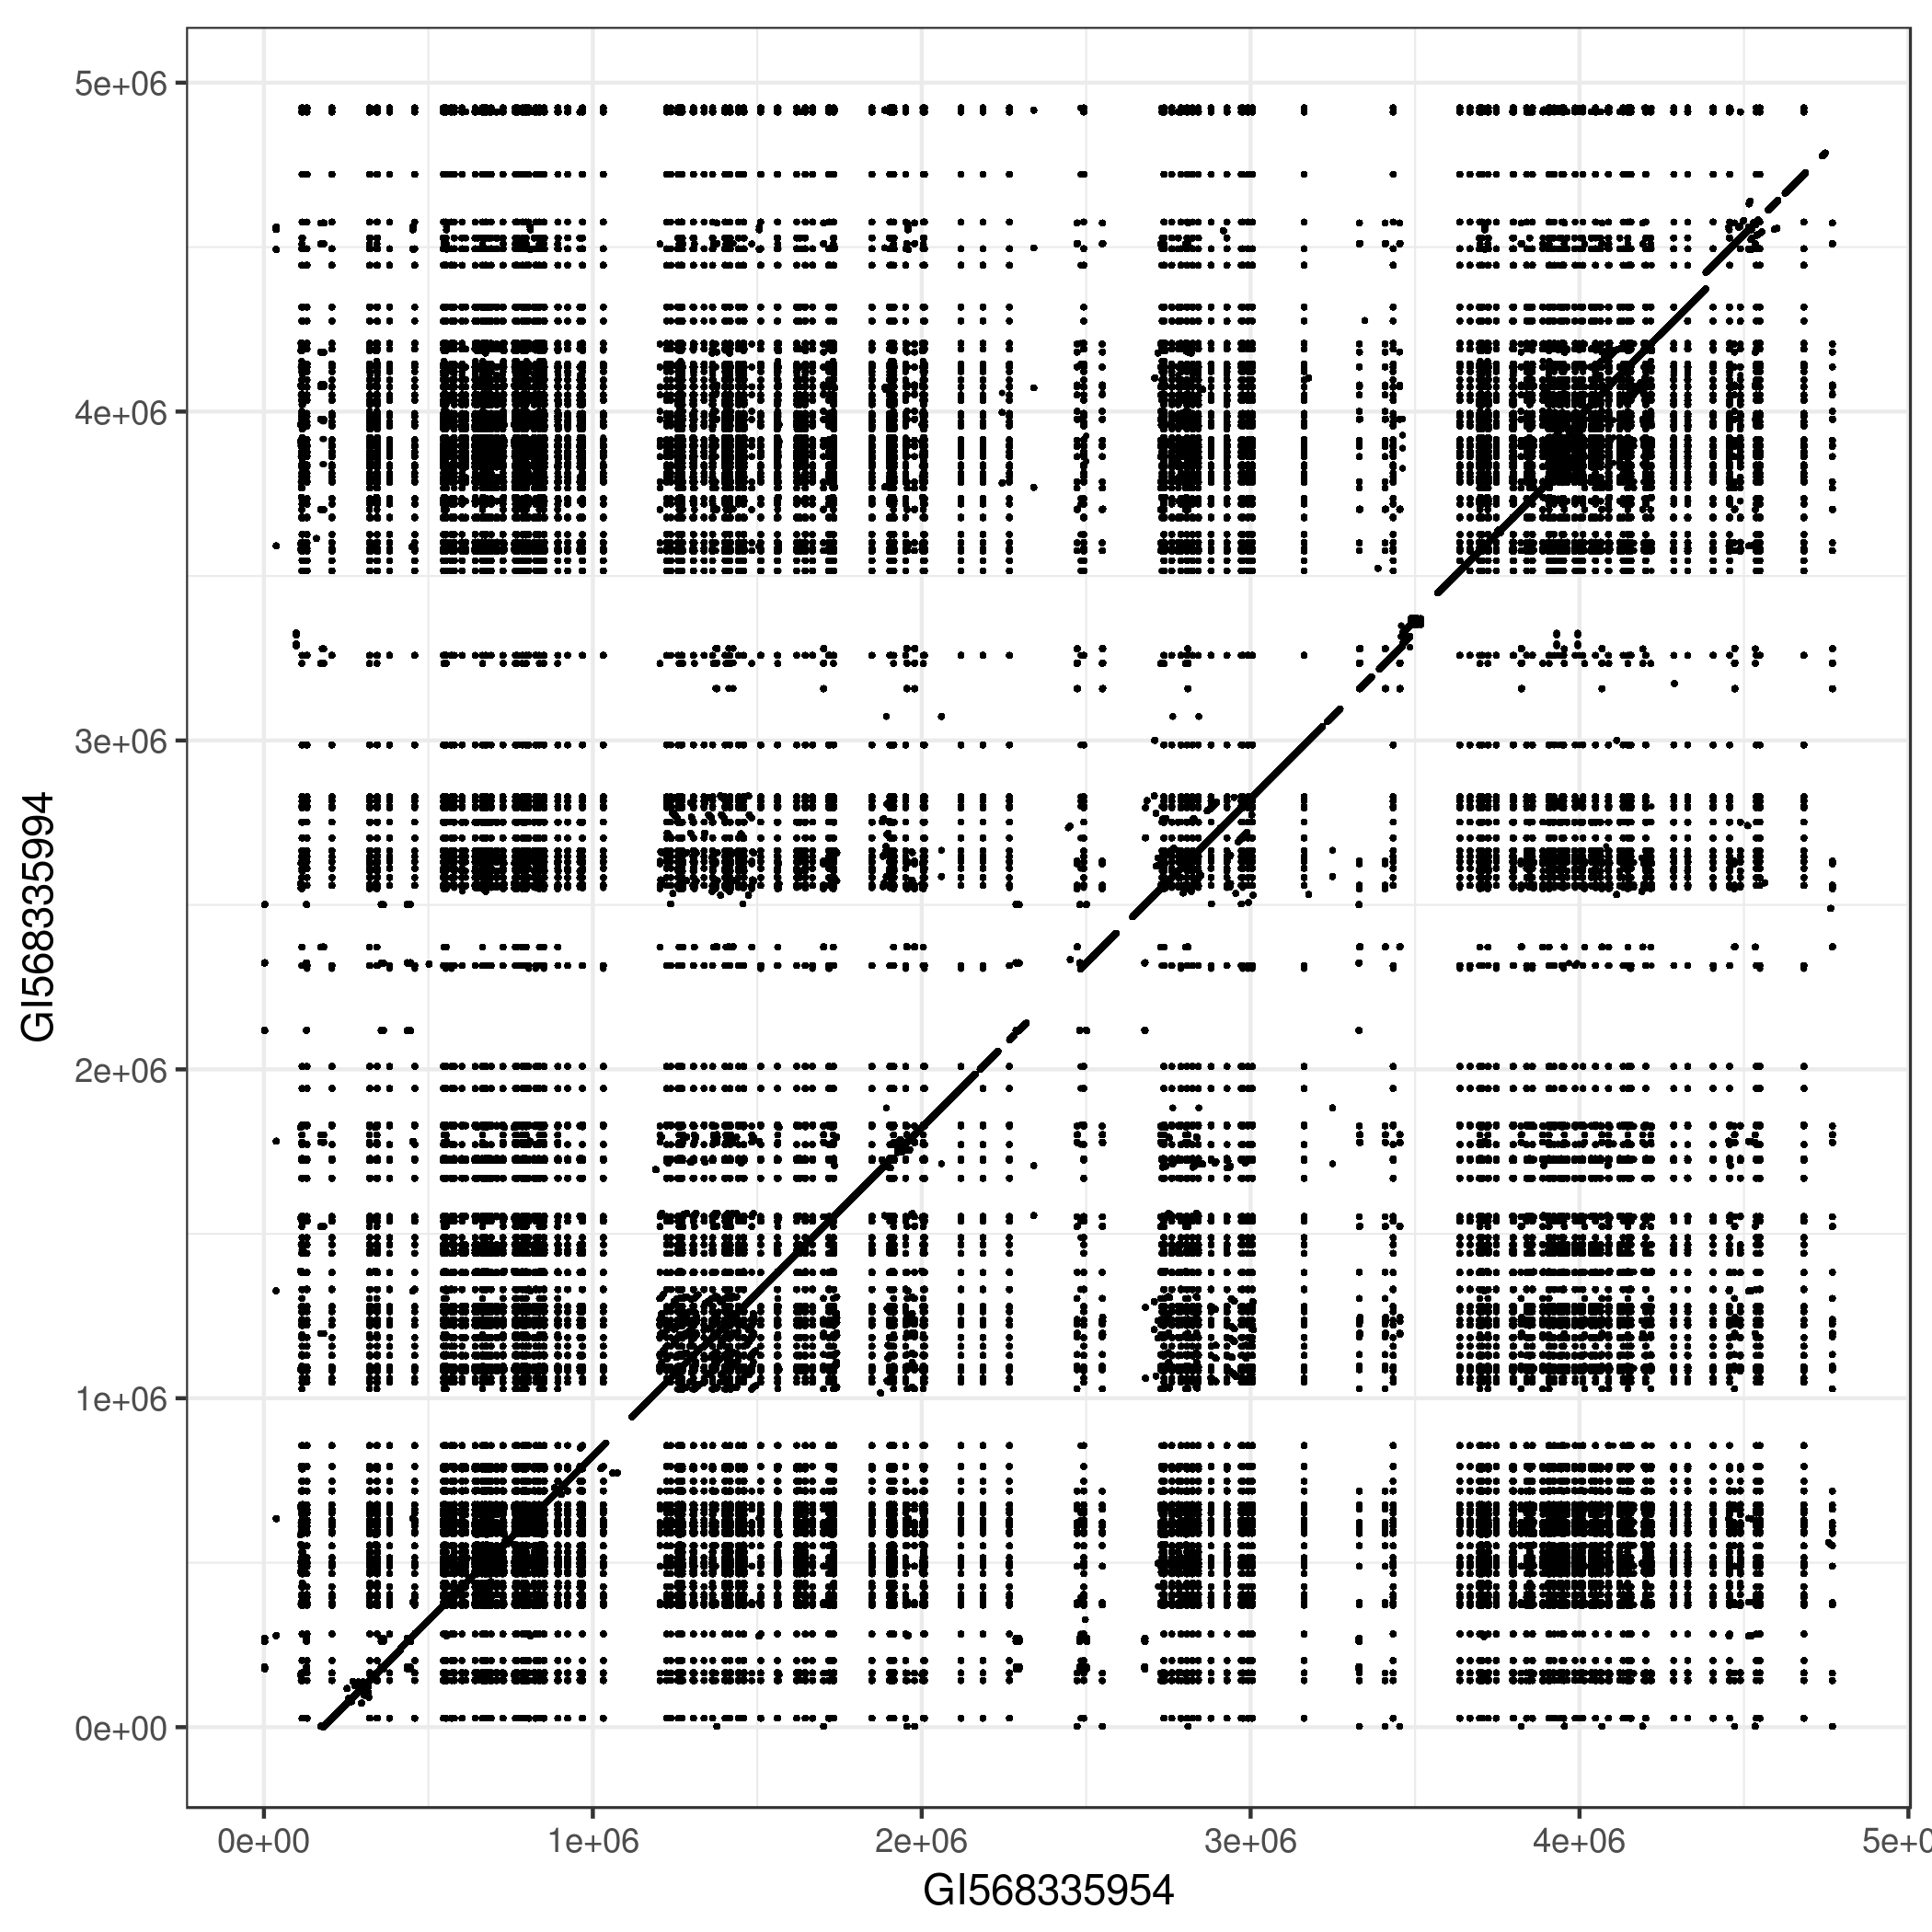
\includegraphics[width=1.0\textwidth]{Chapter3/Figs/seqwish_GI568335954_GI568335994_dotplot.png}
    \caption{{\tt seqwish}}
    \label{subfig:seqwish_mhc_dotplot}
  \end{subfigure}
  \begin{subfigure}[t]{0.49\textwidth}
    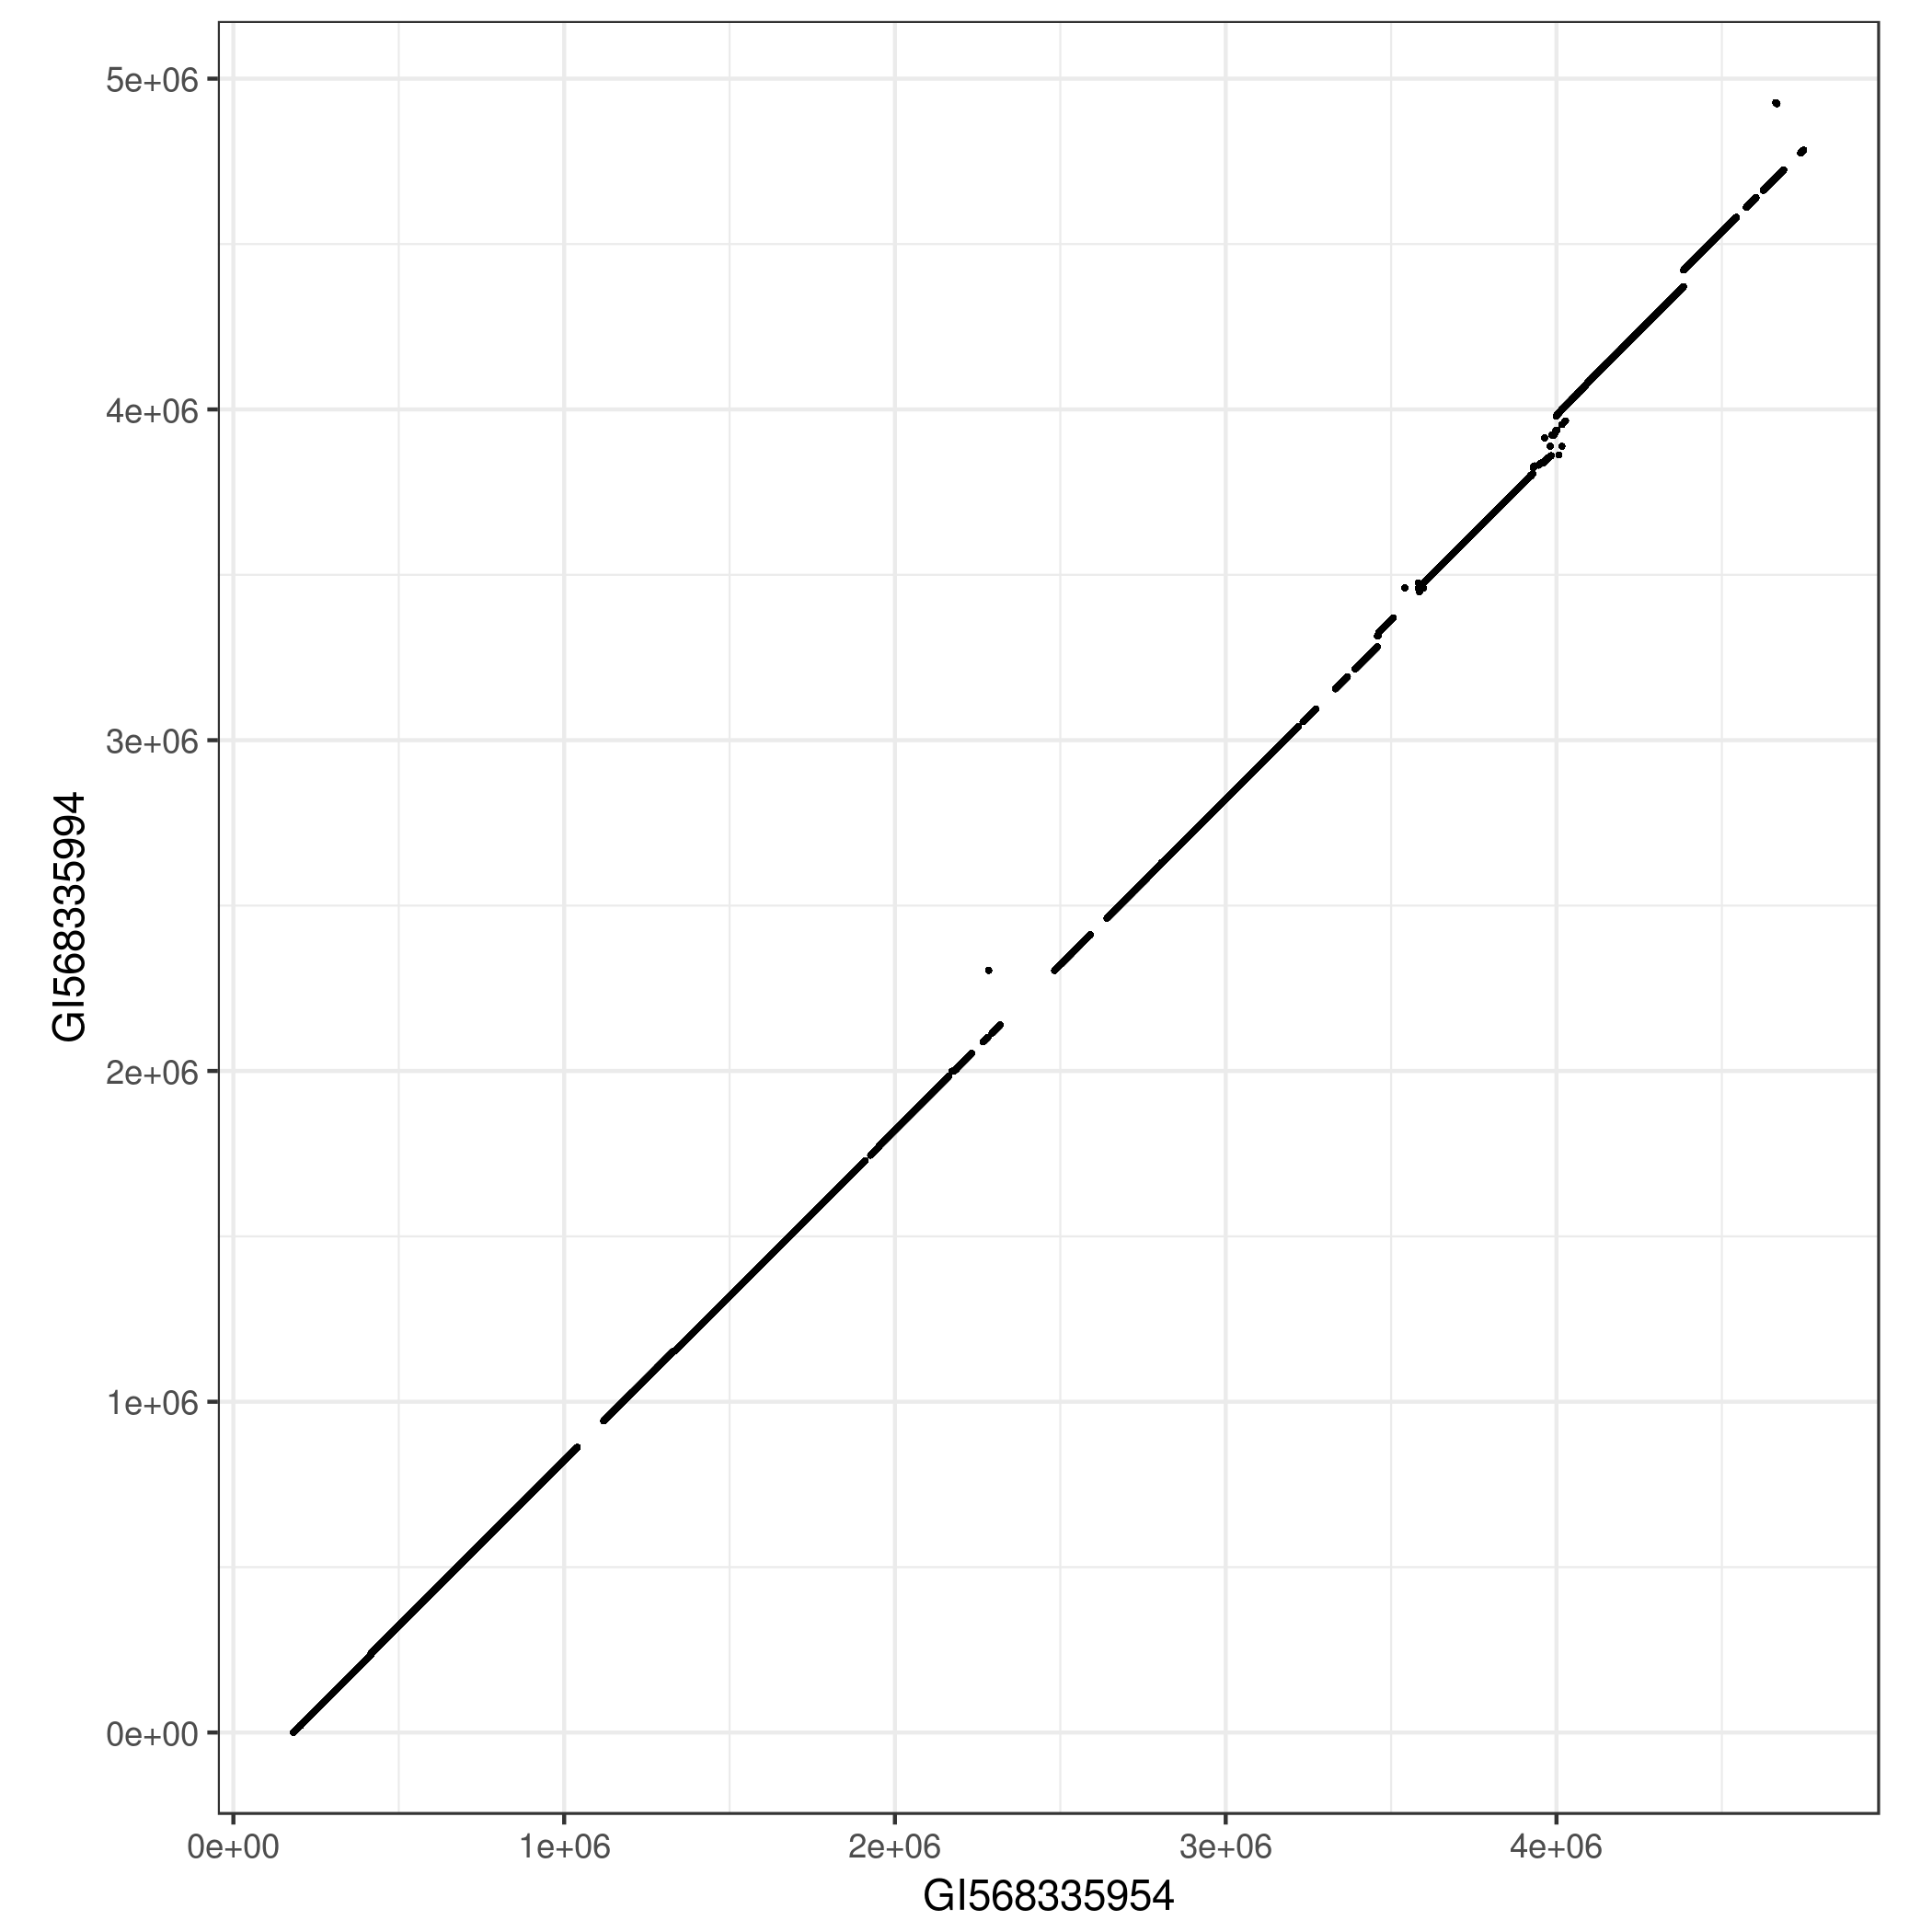
\includegraphics[width=1.0\textwidth]{Chapter3/Figs/vg_msga_GI568335954_GI568335994_dotplot.png}
    \caption{{\tt vg msga}}
    \label{subfig:vg_msga_mhc_dotplot}
  \end{subfigure}
  \caption[Dotplots from assemblies of the MHC in GRCh38.]{
    Comparing {\tt seqwish} and {\tt vg msga} assemblies of the MHC in GRCh38.
    In both panels we see a dotplot between GI568335954 ($x$-axis) and GI568335994 ($y$-axis) as they are embedded in each graph, with \ref{subfig:seqwish_mhc_dotplot} showing the dotplot for {\tt seqwish} and \ref{subfig:vg_msga_mhc_dotplot} that for {\tt vg msga}.
  }
  \label{fig:mhc_dotplots}
\end{figure}

\subsection{CHiP-Seq}
%*1p 1h*

The removal of mapping bias is important when working with functional genomics data such as ChIP-seq data, where allele-specific expression analysis can reveal genetic variation that affects function but is confounded by reference mapping bias \cite{mcdaniell2010heritable}, especially given that read lengths are typically shorter for these experiments.
We compared mapping with {\tt bwa mem} and {\tt vg} for data set ENCFF000ATK from the ENCODE project \cite{encode2012integrated}, which contains 14.9 million 51-bp ChIP-seq reads for the H3K4me1 histone methylation mark from the NA12878 cell line.
When mapping with bwa the ratio of reference to alternate allele matches at heterozygous sites was 1.20, whereas with vg to the 1000GP graph the ratio was 1.01, effectively eliminating reference bias.

\begin{figure}[htbp!] 
  \centering
  \begin{subfigure}[t]{0.49\textwidth}
    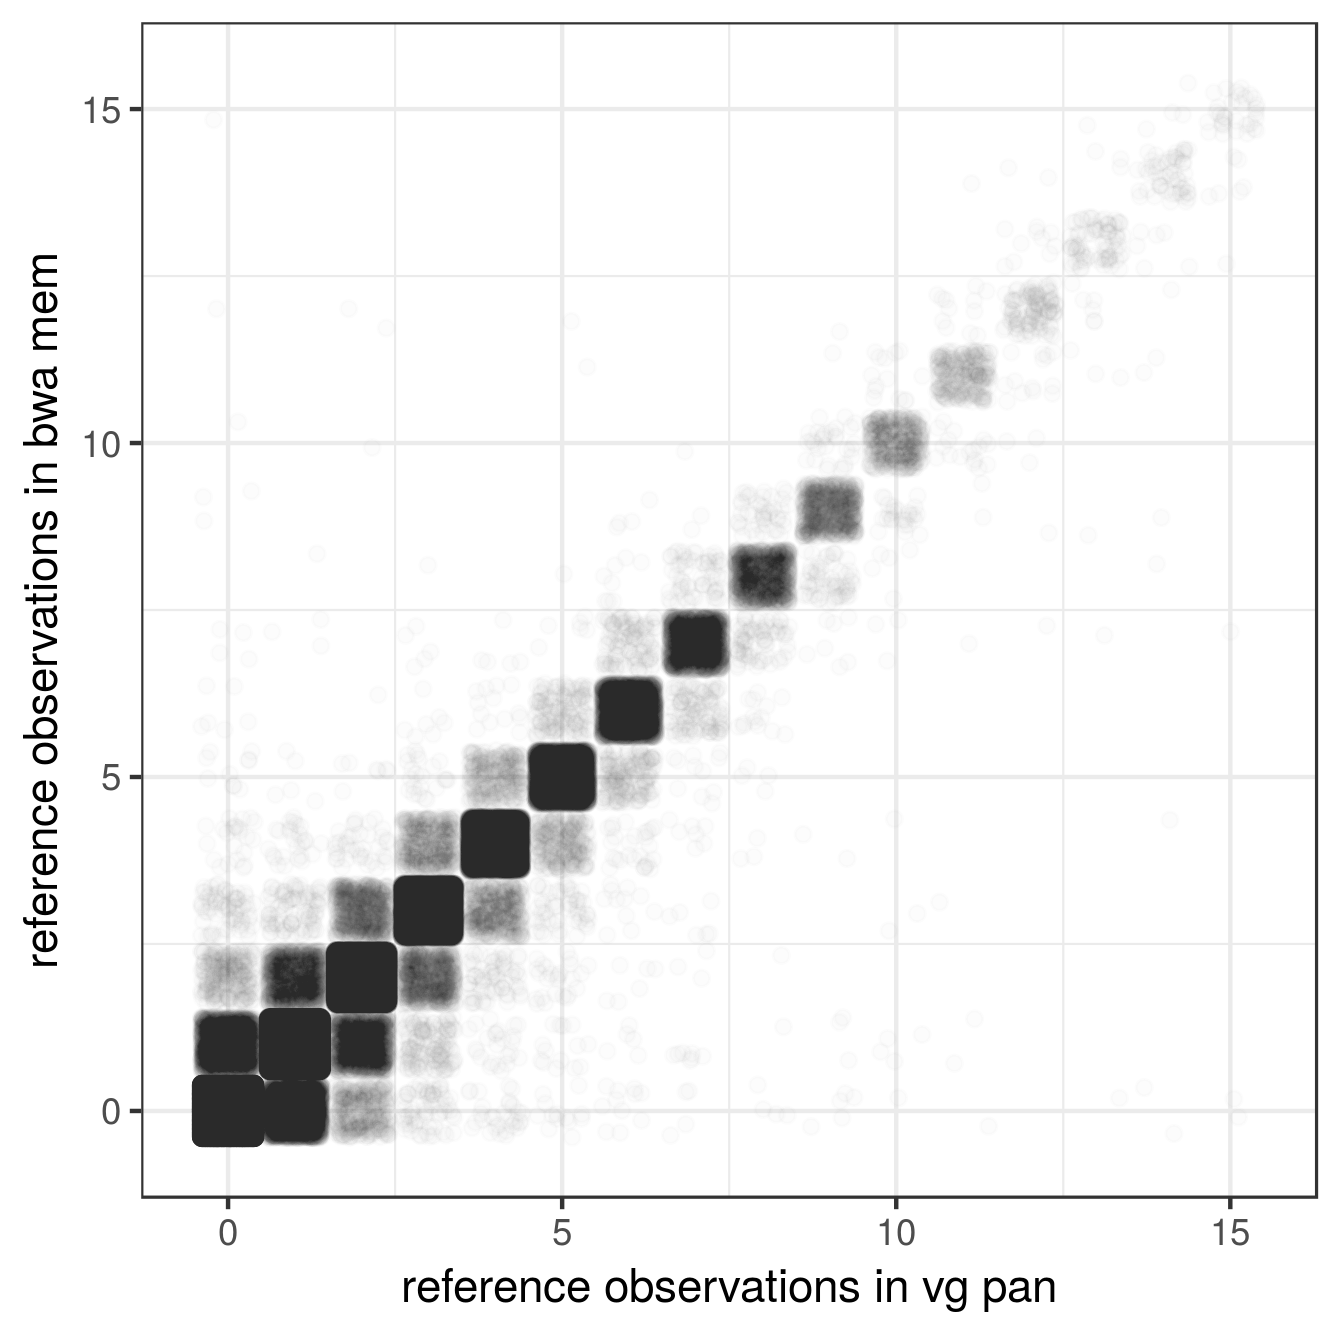
\includegraphics[width=1.0\textwidth]{Chapter3/Figs/ENCFF486KYD_RO_vg_pan_vs_bwa.png}
    \caption{Reference observations}
    \label{subfig:chip_seq_ref_obs}
  \end{subfigure}
  \begin{subfigure}[t]{0.49\textwidth}
    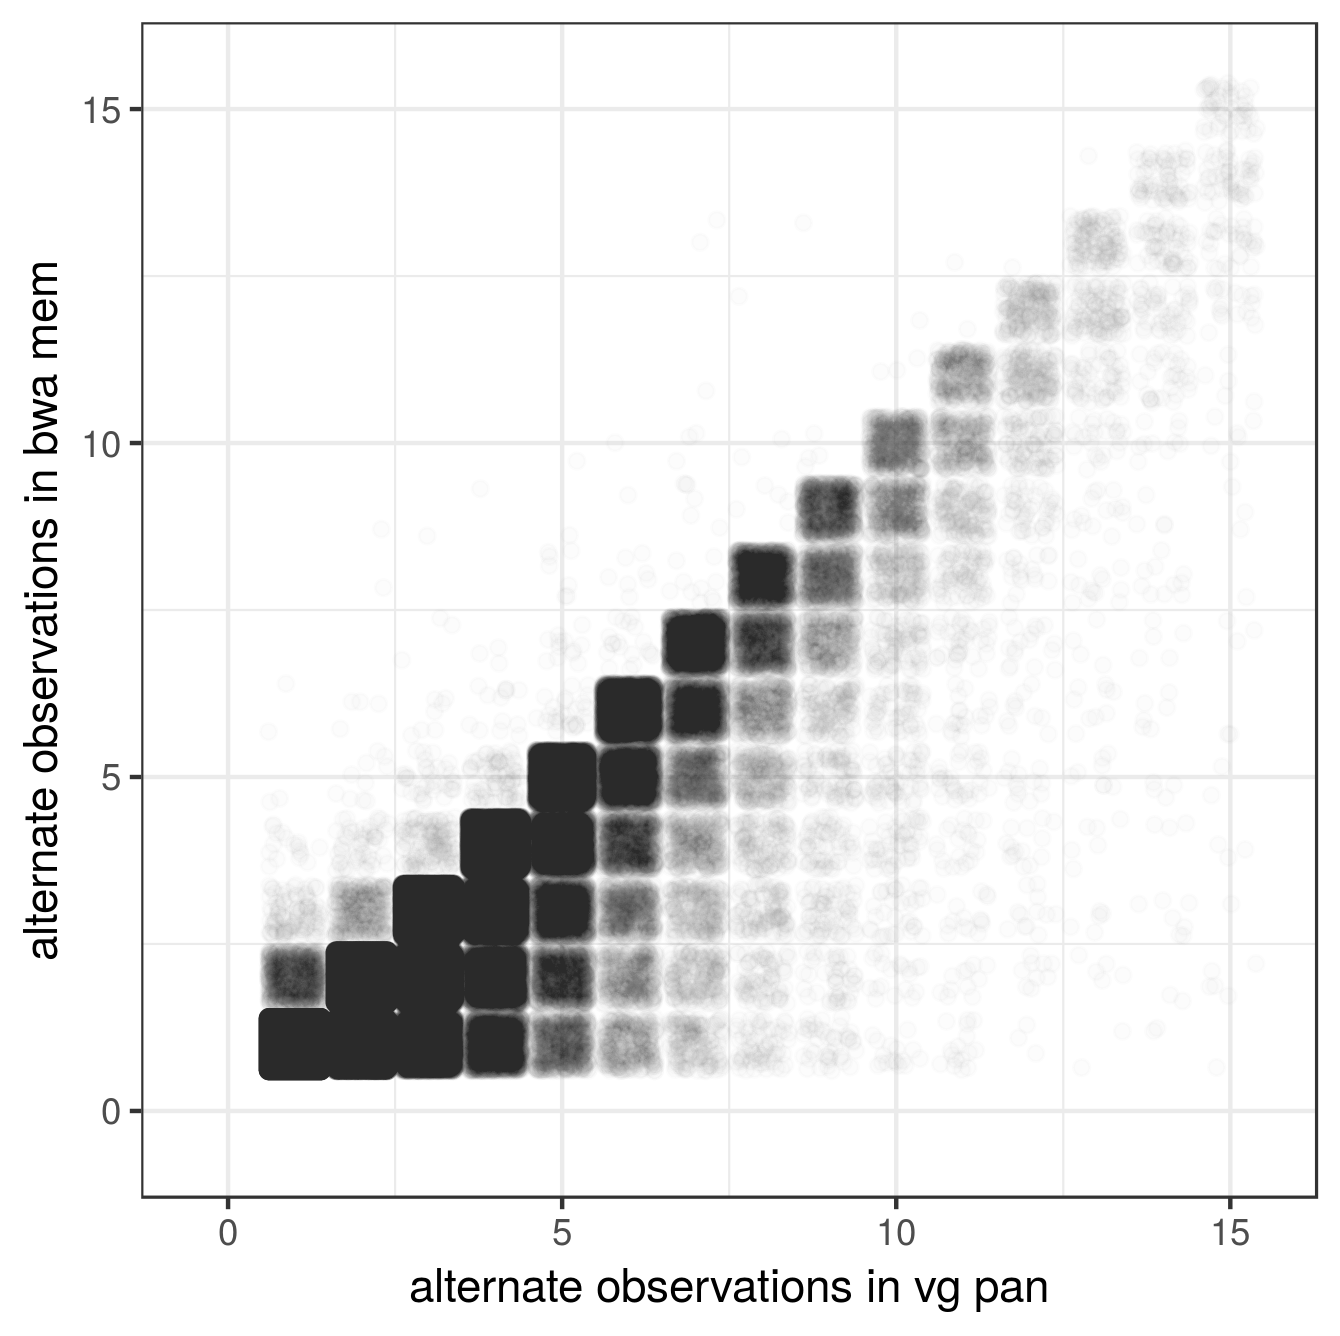
\includegraphics[width=1.0\textwidth]{Chapter3/Figs/ENCFF486KYD_AO_vg_pan_vs_bwa.png}
    \caption{Alternate observations}
    \label{subfig:chip_seq_alt_obs}
  \end{subfigure}
  \caption[Resolving reference bias in 36-bp CHiP-seq]{
    Resolving reference bias in 36-bp CHiP-seq data from ENCODE sample ENCDO115AAA, using CHiP-seq targeting H3K4me1 (experiment ENCFF000ATK).
    We compare the counts of reference-supporting (panel \ref{subfig:chip_seq_ref_obs}) or alternate-supporting (panel \ref{subfig:chip_seq_alt_obs}) alignments between {\tt vg map} and {\tt bwa mem} at sites called as heterozygous in the sample which were also polymorphic in the 1000GP.
    To shown density we have jittered the points in the unit square centered on the integral values taken by the counts.
   }
\label{fig:chip_seq}
\end{figure}

The effect is dramatically stronger when using 36-bp reads.
To illustrate, I aligned the ultra-short reads from ENCODE experiment ENCSR290YLQ\footnote{\url{https://www.encodeproject.org/experiments/ENCSR290YLQ/}} to the full 1000GP graph using {\tt vg map} and to the GRCh37 reference genome using {\tt bwa mem}.
To simplify analysis, the {\tt vg} mappings were surjected to the GRCh37 reference.
This sample came from an adult donor, and so we have no ``truth'' set as with NA12878, but we can use a subset of sites called as variable using {\tt freebayes} which also are known to be polymorphic in the 1000GP to examine the effect of reference bias.
By plotting the reference and alternate counts obtained from each aligner relative to each other, we can observe the effect of reference bias on a per-site basis.
I find that {\tt bwa mem} and {\tt vg map} obtain insignificantly different counts of reference observations at the heterozygous sites (panel \ref{subfig:chip_seq_ref_obs}), but as can be seen in panel \ref{subfig:chip_seq_alt_obs}, aligning to the graph uncovers dramatically more alternate observations at these loci, as is shown by the strong increase in density below the diagonal.
The strength of this effect indicates that small variation will disrupt alignment of very short reads of relatively high quality and low error rates.
The issue becomes even more dramatic when we consider data sources with higher error.

\section{Ancient DNA}

In suitable conditions, DNA can survive for tens or even hundreds of thousands of years \emph{ex vivo}, providing a unique window into the past history of life \cite{dabney2013ancient}.
However, the sequencing analysis of Ancient DNA poses several significant challenges.
The amount of DNA available is often limited, and sequencing costs are increased in the presence of high rates of contamination by organisms that inhabit the sample after its death.
Read lengths are limited by the degradation of DNA due to necrotic processes and subsequent environmental exposure.
Post-mortem damage (PMD) of the DNA occurs at a high rate, introducing mutations in the tails of the short DNA molecules, which occur in a single-stranded and relatively unprotected state \cite{link2017atlas}.
This manifests mostly as the conversion of cytosines to uracil, but also can lead to apurination \cite{dabney2013ancient}.
Ancient DNA data is thus often of short length, low coverage, and high intrinsic error rate.

In combination these issues cause a strong bias against non-reference variation, which can have a significant effect on population genetic inference and implications for many aDNA studies.
Ancient DNA may be treated with uracil-DNA-glycosylase (UDG) and endonuclease VIII to remove uracil residues and abasic sites, leaving undamaged portions of the DNA fragments intact \cite{briggs2009removal}.
However, this process results in a reduction of read length and library depth, which is disadvantageous, and it is not guaranteed to proceed without introducing new bias.
There have also been many attempts to mitigate the effects of reference bias and low coverage, such as by implementing a model of reference bias in gentoyping \cite{pruefer2018snpad}, or by working with genotype likelihoods throughout all downstream population genetic analyses \cite{link2017atlas}.
To avoid genotyping or even the generation of genotype likelihoods, standard practice often involves modeling each genome as a collection of haploid chromosomes modeled by reads.

Here I report on the results of an ongoing collaboration with Rui Martiniano and Eppie Jones to explore the use of {\tt vg} to mitigate reference bias in ancient DNA samples.
They have completed most of the analyses, while I have supported their work and developed the alignment (and surjection) algorithms that are essential to them.

\subsection{Evaluating reference bias in aDNA using simulation}

Using simulation, Eppie Jones and I completed an exploratory analysis which demonstrates that the high degree of reference bias inherent in ancient DNA analysis may be mitigated at known sites by aligning against a pangenome graph.
We simulated all possible 50 bp reads which spanned variant sites on chromosome 11 of the Human Origins SNP panel \cite{patterson2012ancient,lazaridis2014ancient}, which is a set of SNPs designed to be highly informative about ancient genomes and human ancestors.
In half of the simulated reads the SNP position was mutated to the alternate allele.
We then mapped these reads back to the 1000GP graph or GRCh37 linear genome using {\tt vg map} and {\tt bwa aln} respectively, with {\tt vg}'s surjection process used to produce a BAM file from the alignment for direct comparison.
Different levels of ancient DNA damage estimated using 100 ancient genomes from \cite{allentoft2015population} were simulated in these data using {\tt gargammel} \cite{renaud2016gargammel}.
We filtered the resulting alignments for those above mapping quality 30, which has approximately the same significance in both {\tt vg} and {\tt bwa}.
Our results are shown in figure \ref{fig:aDNA_simulations}.

\begin{figure}[htbp!]
  \centering
  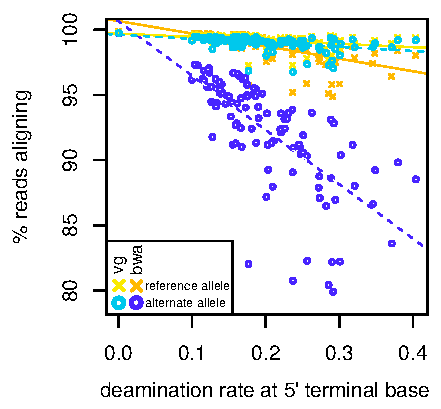
\includegraphics[width=0.7\textwidth]{Chapter3/Figs/bwa_vs_vg_ancient_data_simulations_mq30_recolored.pdf}
  \caption[Comparing {\tt bwa aln} and {\tt vg map} using simulated ancient DNA]{
    Comparing {\tt bwa aln} and {\tt vg map} performance when aligning reads simulated from chromosome 11 of the Human Origins panel.
    Lines represent OLS regression results for the allele/aligner conditions corresponding to their colors.
  }
  \label{fig:aDNA_simulations}
\end{figure}

At high levels of error, alignment against the linear reference prevents the observation of non-reference alleles in a large fraction of cases.
This effect is notable at deamination rates as low as 10\%, and with 30\% PMD error the rate of alignment to non-reference alleles is reduced by nearly 15\% relative to the total.
While {\tt bwa aln} suffers a significant reference bias with increasing simulated PMD rates (dashed dark blue versus orange fit lines representing alternate and reference alleles), we observe no such effect for {\tt vg map} (light blue and yellow) (figure \ref{fig:aDNA_simulations}).
Most of the alleles in the Human Origins panel are also in the 1000GP, which suggests that modern sources are useful when constructing a pangenomic reference for ancient samples.

\subsection{Aligning ancient samples against the 1000GP pangenome}
%*2p 4h*

To evaluate whether pangenomic read mapping techniques could mitigate reference bias in real samples, we collected data from a number of recently published ancient DNA studies.
This includes Iron Age, Roman, and Anglo-Saxon individuals sequenced at low coverage in \cite{schiffels2016iron} and \cite{martiniano2016genomic}, and high-coverage Yamnaya and Botai individuals from \cite{de2018first}.
We used {\tt vg map} to align the samples to the 1000GP pangenome of variants above 0.1\% frequency, and {\tt bwa aln} to align them to the GRCh37 reference plus decoys, using standard parameters for the analysis of ancient DNA ({\tt -l1024 -q15 -n0.02}).
For both alignment results we filtered the resulting BAMs using {\tt samtools view -q30} to remove reads with mapping quality less than 30, and removed duplicates using {\tt sambamba markdup} \cite{tarasov2015sambamba}.

We first considered the high-coverage Yamnaya sample from \cite{de2018first}, which provides approximately 20-fold coverage of the genome.
This is very high for ancient samples and thus allows us to complete some experiments which would be otherwise very difficult.
We called variants on chromosome 21 using bcftools \cite{li2009sequence} for both {\tt vg} and {\tt bwa} alignments.
To evaluate the effect of reference bias with decreasing coverage, we then used these callsets as ground truth and measured our ability to recover the heterozygous variants in the full coverage set at coverage levels of 0.1, 0.2, 0.3, 0.4, 0.5 of the original.
As seen in figure \ref{fig:aDNA_downsampling}, at lower coverages common in ancient DNA sequencing, {\tt bwa aln} recovers notably fewer heterozygous SNPs than {\tt vg map} alignment to the 1000GP graph.
At the sampling rate of 0.2, which corresponds to coverage $\approx$4, {\tt vg map} recovers 8\% more heterozygotes as a fraction of the total.
{\tt vg map} recovers more heterozygous SNPs than {\tt bwa aln} at all the coverage levels, although at higher levels the difference is less pronounced.
We expect this would have a significant effect on population genetic analyses depending on these alignments.

\begin{figure}[htbp!]
  \centering
  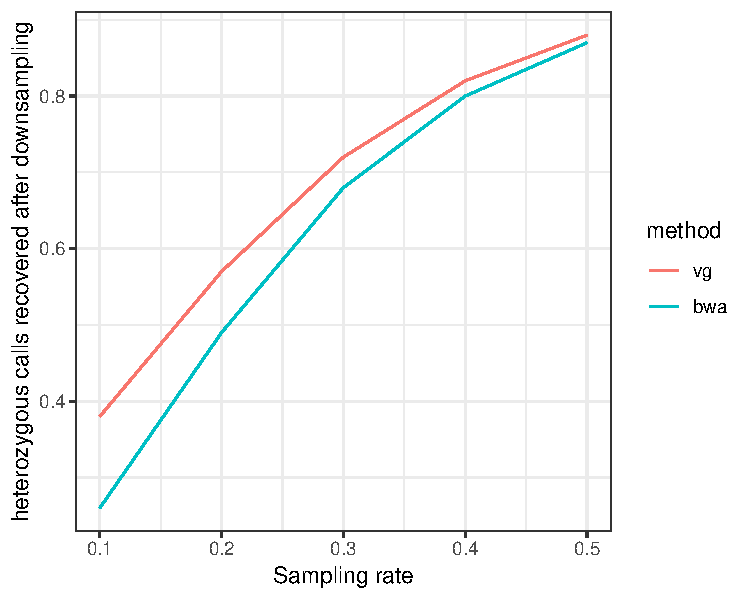
\includegraphics[width=0.7\textwidth]{Chapter3/Figs/aDNA_downsampling.pdf}
  \caption[Downsampling a high-coverage aDNA sample]{
    The comparative effect of downsampling of an ancient DNA sample on {\tt bwa aln} and {\tt vg map} alignment.
  }
  \label{fig:aDNA_downsampling}
\end{figure}

In an illustrative, if less well-controlled experiment, we simply examined the distribution of the ratio between reference and alternate allele observations in the set of variants called by {\tt freebayes} from the surjected {\tt vg map} Yamnaya alignments.
We first subset the called alleles into heterozygous transversions, and further divided the resulting set of putative transversions into those alleles in the 1000GP graph, and those which are not.
As shown in figure \ref{fig:yamnaya_het_violins}, we observe that if the variant is in the graph (N $\approx$ 1M) we have effectively removed bias towards the reference allele.
This is not the case for those called alleles (N $\approx$ 300K) which are not in the graph.

%  get 1.3M, of which 1M are in the 1000GP set

\begin{figure}[htbp!]
  \centering
  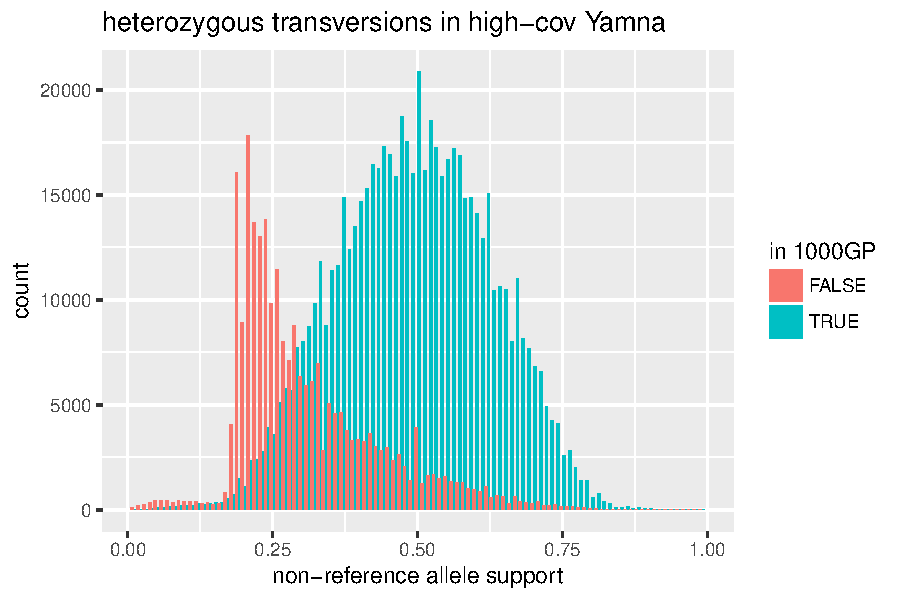
\includegraphics[width=0.7\textwidth]{Chapter3/Figs/yamna_1000GP_AB_het_hist.pdf}
  \caption[Allele balance in the Yamnaya sample]{
    Allele balance in the {\tt vg} alignment of the Yamnaya sample to the 1000GP graph versus its presence in the 1000GP graph.
  }
  \label{fig:yamnaya_het_violins}
\end{figure}

We expect reference bias of the degree demonstrated in these experiments to affect population genetic inference.
To evaluate this, we apply the ABBA BABA test of phylogenetic tree topology based on Patterson's $D$-statistic of population relationship \cite{green2010draft}.
To do so, we used the Human Origins dataset distributed with \cite{lazaridis2014ancient}.
For each sample we ran samtools pileup yielding ~1.2 million SNPs.
We converted the pileup results to plink format, selecting one allele at random from the confidently mapped reads spanning each site, as is standard in the field.
This was done 5 times, generating 5 replicates of randomly selected alleles for each sample.
We then filtered by genotyping rate, excluding poorly genotyped SNPs\footnote{We used the plink filter {\tt --geno 0.05}.}, resulting in 1,142,867 SNPs.
Finally, we merged individual plink files with those for GRCh37 and Chimpanzee, converted plink to eigenstrat format using {\tt convertf} and calculated $D$-statistics using qpDstat \cite{patterson2012ancient} of the form $D(\text{vg}, \text{bwa}; \text{GRCh37}, \text{Chimp})$ to test for excess of shared alleles between {\tt vg} and {\tt bwa}-aligned samples with the reference.

\begin{figure}[htbp!]
  \centering
  \begin{subfigure}[t]{0.49\textwidth}
    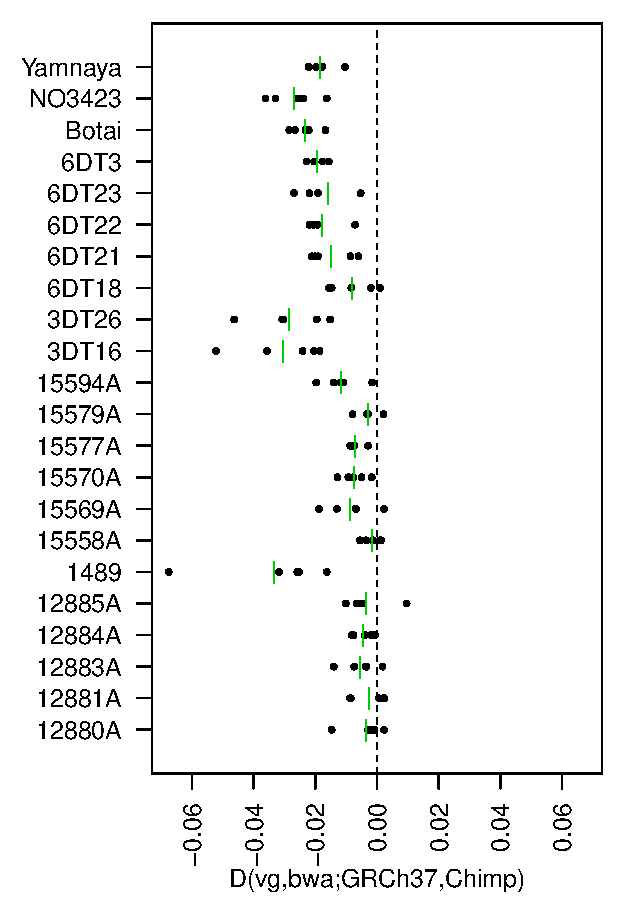
\includegraphics[width=1.0\textwidth]{Chapter3/Figs/aDNA_d_stats_absolute.pdf}
    \caption{$D$-statistic absolute values}
    \label{subfig:aDNA_dstats_absolute}
  \end{subfigure}
  \begin{subfigure}[t]{0.49\textwidth}
    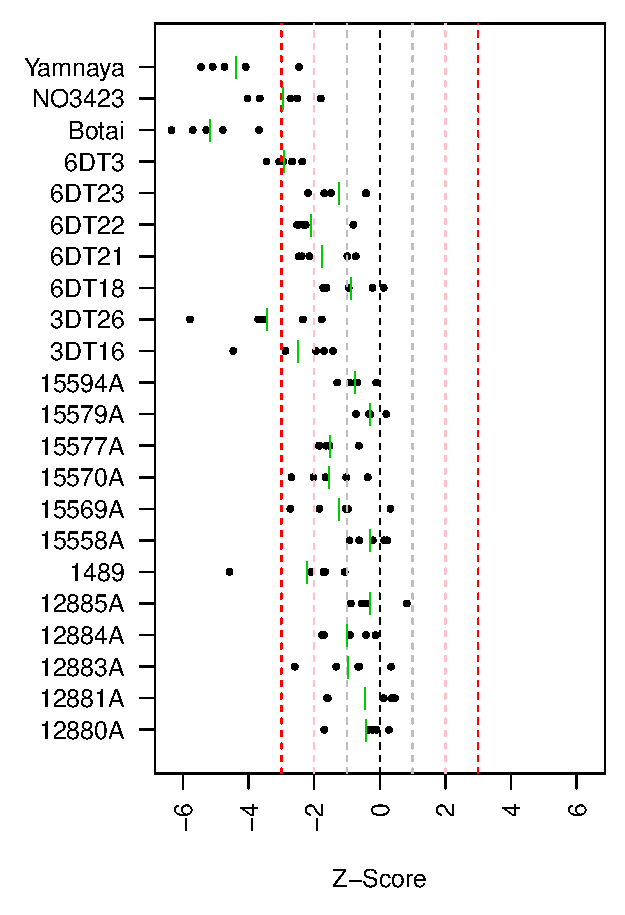
\includegraphics[width=1.0\textwidth]{Chapter3/Figs/aDNA_d_stats_z_score.pdf}
    \caption{$D$-statistic z-scores}
    \label{subfig:aDNA_dstats_zscore}
  \end{subfigure}
  \caption[$D$-statistic based ABBA-BABA test of reference bias in aDNA]{
    $D$-statistic based ABBA-BABA test of reference bias in aDNA.
    Panel \ref{subfig:aDNA_dstats_absolute} provides the absolute values for the given $D$-statistic, calculated as described in the text, while panel \ref{subfig:aDNA_dstats_zscore} shows estimated significance level for the various samples.
    On both panels, points to the left of the dashed line at 0 indicate excess allele sharing between {\tt bwa} alignments of the samples and GRCh37 (the ABBA pattern), while those to the right indicate an excess of sharing between {\tt vg} alignments and GRCh37 (the BABA pattern).
    The two patterns are illustrated by the trees above the panels, where $A$ alleles are given as blue lines on the tree and $B$ alleles that arose between the split with the outgroup (Chimpanzee) are shown in red.
  }
\label{fig:aDNA_dstats}
\end{figure}

Our results, summarized in figure \ref{fig:aDNA_dstats}, indicate an excess of allele sharing between the {\tt bwa}-aligned samples and GRCh37 relative to the {\tt vg}-aligned ones and GRCh37.
All but a handful of replicates have negative $D$-statistics, which implies that alignment against GRCh37 makes the samples appear more like the reference (subfigure \ref{subfig:aDNA_dstats_absolute}).
We conclude that reference bias is strong enough to affect common population genetic analysis completed with ancient DNA, and this can be mitigated at least for known alleles by aligning against a pangenomic reference.

\section{Neoclassical bacterial pangenomics}
%*0.5p 0.5h*

As I discussed in the introduction (section \ref{sec:pangenomes}), during much of the past decade pangenomic concepts have been employed in microbiology to characterize the relationship between strains that frequently share DNA through horizontal gene transfer and exhibit wide variability in gene content.
It is often helpful to consider the ``core'' and ``accessory'' pangenome of a given clade, with core genes being those present in all strains and accessory ones those present in only a subset.
Techniques to evaluate these features of a pangenome are often based on gene counting approaches that can be driven by simple $k$-mer matching.

In this section I demonstrate that {\tt vg} can be applied to derive the same kind of result by directly working on a pangenome graph reference built from diverse strains of \emph{Escheria coli}\footnote{I developed this technique during the Computational Pangenomics (CPANG18) course at the Instituto Gulbenkian de Ci\'{e}ncia in Oieras, Portugal. See \url{https://gtpb.github.io/CPANG18/}. This particular practical was explored on the third day of the course \url{https://gtpb.github.io/CPANG18/pages/bacteria.html}.}.
The basic idea is to build a pangenome using a standard DBG assembler, then align all the strain level data we have available against the resulting assembly graph. 
The advance that {\tt vg} offers is precision.
Rather than considering gene-level counts, alignment with {\tt vg} provides per-base, per-sample coverage information.
The results can be used as in resequencing to find new variants, and to genotype existing ones in the graph.
This approach is similar to colored de Bruijn graphs \cite{iqbal2013}, but it allows for out-of-core computation, retains full alignment information, and is consequently (in principle) lossless with respect to the input reads.

\begin{figure}[htbp!]
  \centering
  \begin{subfigure}[t]{1.0\textwidth}
    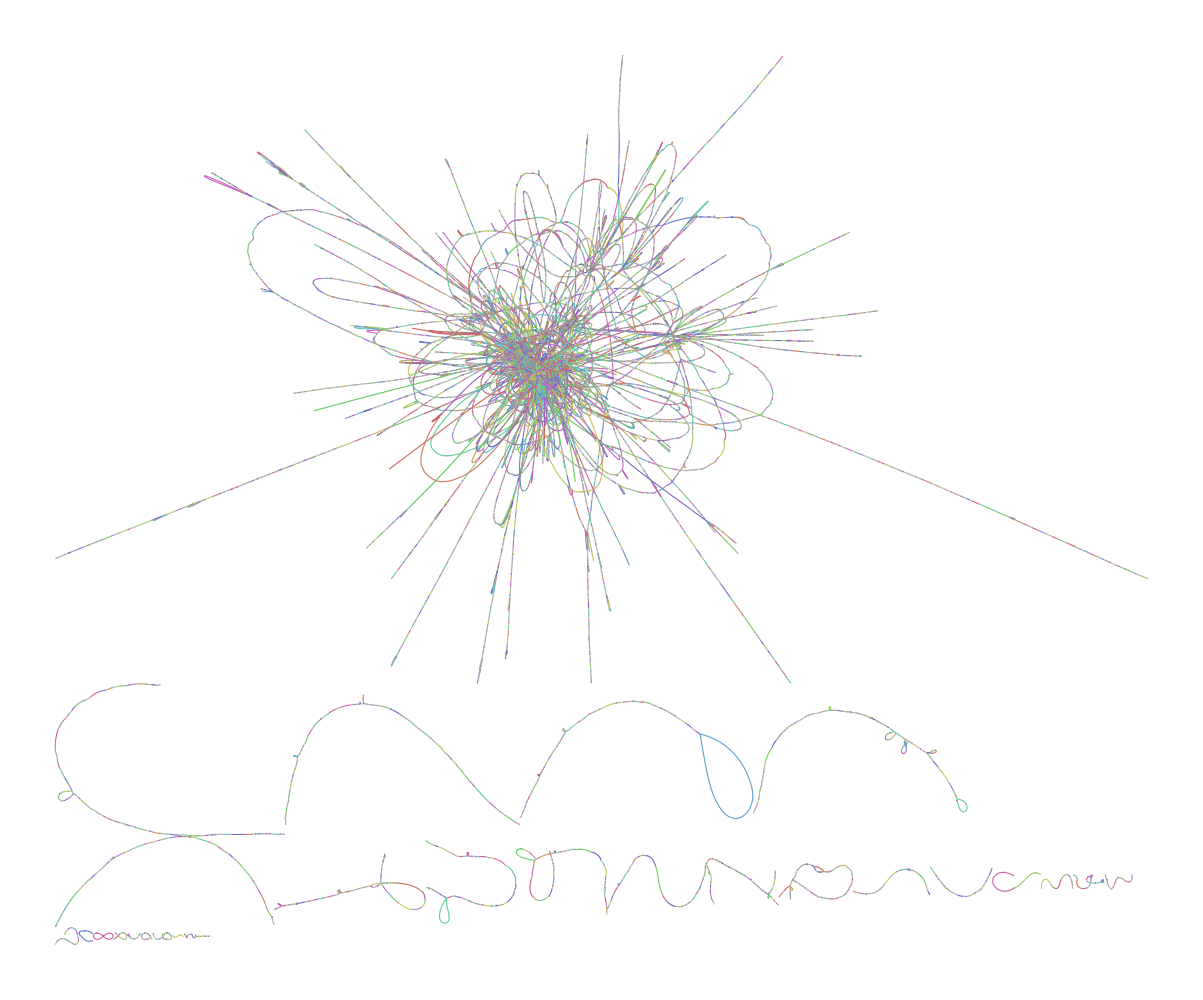
\includegraphics[width=1.0\textwidth]{Chapter3/Figs/ecoli_10strain_kmer51abund10_contigs_vg_gfa.png}
    \caption{The full \emph{E. coli} assembly graph.}
    \label{subfig:ecoli_pangenome_bandage}
  \end{subfigure}
  \begin{subfigure}[t]{0.7\textwidth}
    \includegraphics[width=1.0\textwidth]{Chapter3/Figs/ecoli_n298051_c100.pdf}
    \caption{A linear region of the assembly graph, with variation.}
    \label{subfig:ecoli_pangenome_linear}
  \end{subfigure}
  \begin{subfigure}[t]{0.7\textwidth}
    \includegraphics[width=1.0\textwidth]{Chapter3/Figs/ecoli_n213909_c100.pdf}
    \caption{A semi-tangled region of the assembly graph.}
    \label{subfig:ecoli_pangenome_tangle}
  \end{subfigure}
  \caption[An \emph{E. coli} pangenome]{
    An assembly graph built from 10 \emph{E. coli} strains using minia.
    In the full graph we observe a single giant component (panel \ref{subfig:ecoli_pangenome_bandage}).
    The graph is largely linear (\ref{subfig:ecoli_pangenome_linear}).
    However, in some regions it is densely tangled (\ref{subfig:ecoli_pangenome_tangle}).
  }
  \label{fig:ecoli_pangenome}
\end{figure}


\subsection{An \emph{E. coli} pangenome assembly}
%*2p 4h*

In line with early work on bacterial pangenomics \cite{medini2005microbial}, I used a handful of genomes to demonstrate the utility of pangenomic approaches in \emph{E. coli}.
I collected Illumina data from 10 strains published in \cite{earle2016identifying}\footnote{SRA accessions SRR3050857, SRR3050919, SRR3050929, SRR3050978, SRR3050990, SRR3050992, SRR3050994, SRR3051002, SRR3051049, and SRR3051079.}.
These data total 2.3GB of compressed FASTQ in 2x151bp paired end format.
I built a compressed DBG using {\tt minia} with $k=51$ and an abundance minimum of 10, which was selected due to the very high genomic coverage offered by this data, although I did not observe large changes in assembly structure when varying it.
I then processed the resulting graph with {\tt vg} to decompress long nodes into nodes with a maximum length of 32bp, then sort it pseudotopologically and compact its node identifier space.
These steps are required for efficient mapping given the absence of any annotated reference paths to provide distance estimates.
As seen in figure \ref{fig:ecoli_pangenome}, the assembly graph features a giant component representing most of the input sequencing data.
Other fragments could represent plasmids or other contaminating elements.
The normalized graph contains 10,456,557bp of sequence, in 429,377 nodes and 455,892 edges.
The facts that the average node length is over 24bp and that there are only 1.06 edges per node suggest that despite its tangled appearance, it is mostly composed of linear components.
The assembly and indexing of the graph was completed in less than an hour, and yielded 6.3MB {\tt vg} graph, a 37MB {\tt xg} index, and a 47MB {\tt GCSA2} index.

\subsection{Evaluating the core and accessory pangenome}

The generation of the compressed DBG loses the read-level relationships to the graph, but these may be obtained trivially with {\tt vg} by aligning the read set back to the assembly graph.
Doing so required around 5 minutes per sample, yielding 3.3GB of GAM files in around an hour.
To obtain coverage counts per sample across the graph I then applied the {\tt vg pack} utility to project the alignment GAMs into coverage maps for each sample, which I collated for processing in R.


\begin{figure}[htbp!]
  \centering
  \begin{subfigure}[t]{1.0\textwidth}
    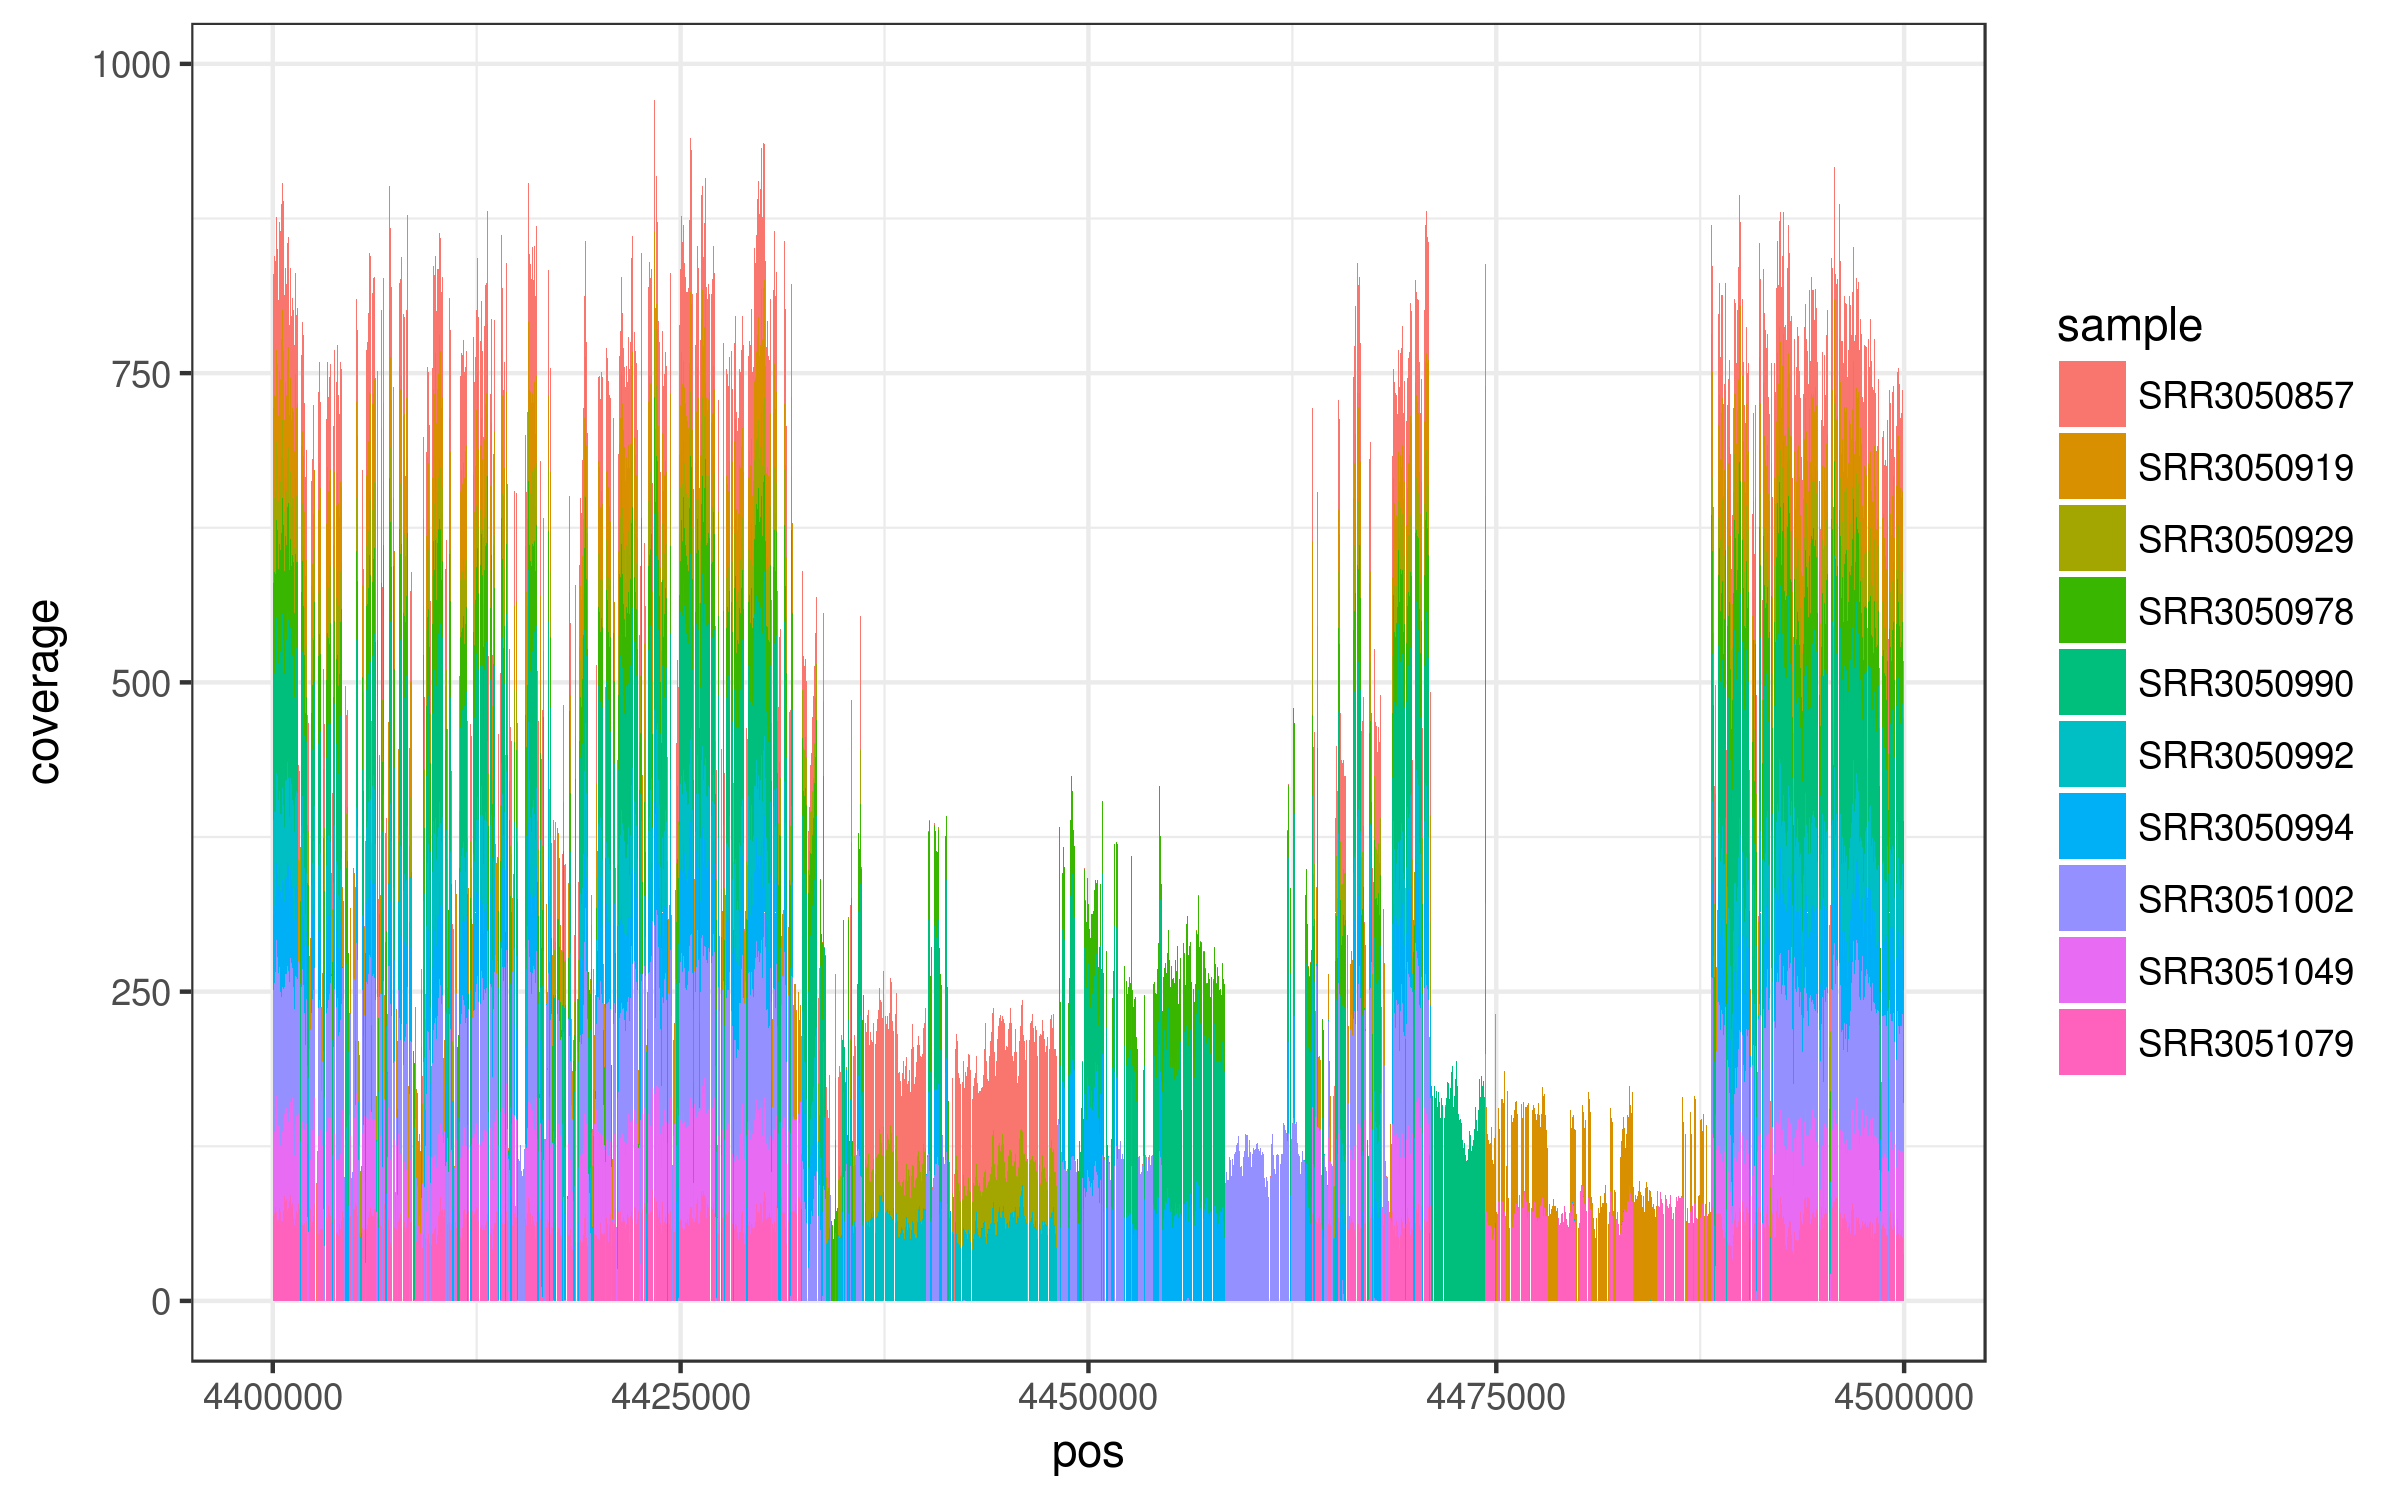
\includegraphics[width=1.0\textwidth]{Chapter3/Figs/ecoli_10strain_cov_col_pos_4400000_100k.png}
    \caption{Per-strain coverage across 100kb of the \emph{E. coli} pangenome}
    \label{subfig:ecoli_cov_100k}
  \end{subfigure}
  \begin{subfigure}[t]{0.49\textwidth}
    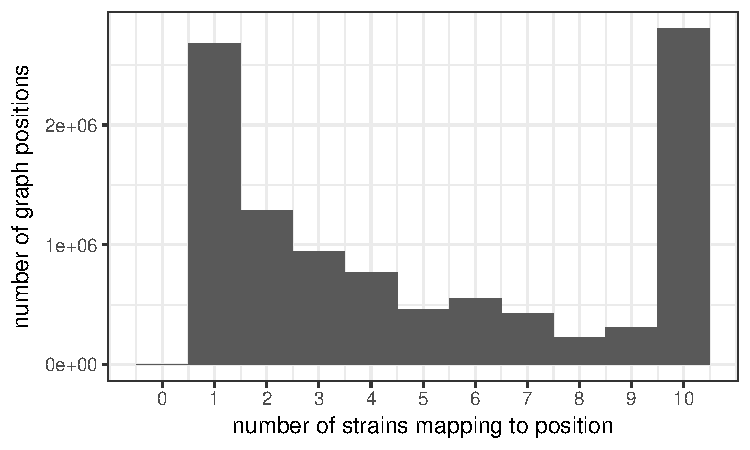
\includegraphics[width=1.0\textwidth]{Chapter3/Figs/ecoli_cov_strains_hist.pdf}
    \caption{Genomes per base of the pangenome}
    \label{subfig:ecoli_cov_strains}
  \end{subfigure}
  \begin{subfigure}[t]{0.49\textwidth}
    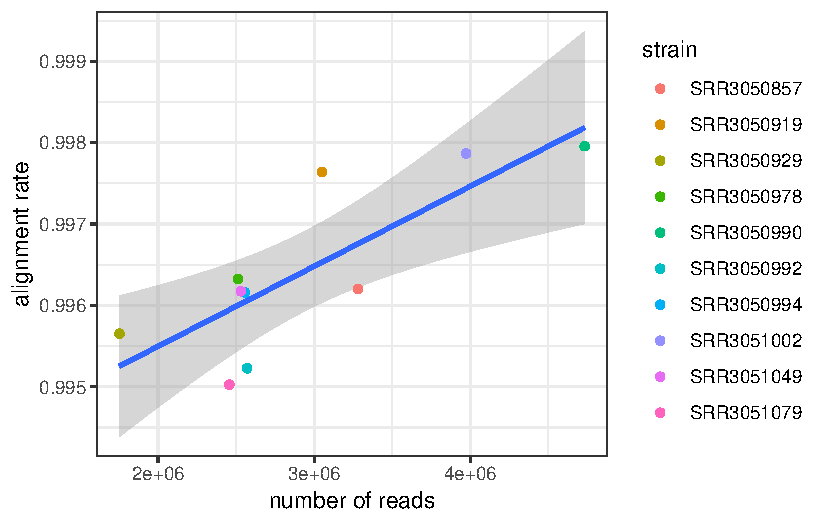
\includegraphics[width=1.0\textwidth]{Chapter3/Figs/ecoli_pangenome_alignment_rate_vs_depth.pdf}
    \caption{Realignment rate versus input read count}
    \label{subfig:ecoli_realignment_vs_input}
  \end{subfigure}
  \caption[Evaluating alignment to the \emph{E. coli} pangenome.]{
    Evaluating alignment to the \emph{E. coli} pangenome.
    Panel \ref{subfig:ecoli_cov_100k} shows per-strain coverage across a selected region of the $\approx$10MB pangenome, including several regions specific to a subset of the strains.
    Panel \ref{subfig:ecoli_cov_strains} provides a histogram of the number of genomes covering each base of the pangenome demonstrates that much of the genome is in all strains or in single strains.
    Although the alignment rate of the input reads to the pangenome graph is in all cases is above 99.5\%, we see a significant correlation between this rate and the number of input reads from each strain used to construct the graph (panel \ref{subfig:ecoli_realignment_vs_input}).
  }
  \label{fig:ecoli_pangenome_alignment}
\end{figure}

Figure \ref{subfig:ecoli_cov_100k} shows the coverage across a typical region of the pangenome.
We see regions shared by all strains, as well as others which are particular to a single or small number of strains.
This is exactly in line with our expectations based on observations from ``classical'' bacterial pangenomics.
To quantify this over the whole pangenome, I computed the histogram of graph positions by the number of strains mapping to each position, as summarized in figure \ref{subfig:ecoli_cov_strains}.
I find that 26.9\% of the pangenome is covered by all ten strains, while 25.6\% is covered by only one strain.
The remaining 47.5\% of the pangenome has intermediate numbers of strains mapping to it.
As such we can conclude that around $\frac{1}{4}$ of the pangenome is the conserved ``core,'' and $\frac{1}{4}$ is purely ``accessory,'' occuring in only a single strain.

Virtually all the graph is covered by some strain, with only 80bp receiving no mappings, which indicates that the pangenome object is complete.
However, the read sets are not equivalently contained in the pangenome, and a significant ($p=0.00534$) correlation exists between the realignment rate of the reads to the pangenome and the number of raw reads from each strain, as seen in figure \ref{subfig:ecoli_realignment_vs_input}.
This statistic suggests that a few strain-specific regions are not assembled.
Naturally, the rate at which this failure occurs is dependent on read depth.
It is possible that this effect is driven by the high abundance count (10) used in constructing the compressed DBG, and possibly it could be mitigated by tuning this parameter and the $k$-mer length.

\section{Metagenomics}

\emph{Metagenomics} is conceptually close to pangenomics.
But, where pangenomics considers a single clade, metagenomics considers the total DNA in an environmental context.
This adds significant complexity to the analysis of metagenomic data.
To obtain high coverage across all the extant genomes in a sample may be impossible, as many exist at extremely low copy.
Furthermore, doing so could be extremely expensive.
In response, reductive approaches focused on sequencing 16S ribosomal DNA or other conserved gene sequences have been popular \cite{tringe2005comparative}.
These methods are only applicable where such homologous sequences are available, and so cannot be applied to viral contexts \cite{edwards2005viral}.
As sequencing costs have decreased, assembly techniques have become more important to metagenomics \cite{nurk2017metaspades}.
A typical workflow involves assembling contigs out of a DBG, mapping these contigs into annotated databases using sensitive alignment with BLAT or BLAST, and computing abundance by aligning the read set back to the contig set.
Contigs, in being unary, suppress variation that could be useful in analysis.
Furthermore, in graphs that are dense, contigs will be very short, and linear read alignment will fail to completely capture the set of contigs that a given read maps to.
This will result in distortion in coverage estimates, and at very least loss of information due to the breakage of sequences that cross contigs boundaries.
The information loss suggests that a technique based on alignment to the assembly graph itself could benefit downstream analysis.
In this section I use analyses of viral and bacterial metagenomes to demonstrate that {\tt vg} enables contiguous alignments against topologically complex metagenomic assembly graphs.

\subsection{Arctic viral metagenome}

To explore this issue, I built an assembly graph from a single sequencing data set from a study of freshwater viruses in Svalbard \cite{de2015biodiversity}\footnote{Data from \url{https://www.ebi.ac.uk/ena/data/view/ERS396648}} and compared the performance of alignment against the graph with alignment against the contig set.
As with other assembly graph based variation graphs, I used {\tt minia} to construct the graph, with $k=51$ and a minimum abundance of 3.
To enable efficient alignment against the graph, I chopped its long nodes into nodes of a maximum of 32bp.
The resulting graph has 39,503,775bp of sequence in 1,387,287 nodes and 1,326,573 edges.
The low ratio of edges to nodes suggests a locally linear structure, which enables direct use of the graph by {\tt vg}.
In fact there are fewer edges than nodes, which also means the graph contains many isolated components.
To successfully index the graph I found I had to remove complex regions using {\tt vg prune}, cutting edges that induced 3 bifurcations in any 16-mer.
Indexing yielded a 119MB {\tt xg} index and 158MB {\tt GCSA2} index.

\begin{figure}[htbp!]
  \centering
  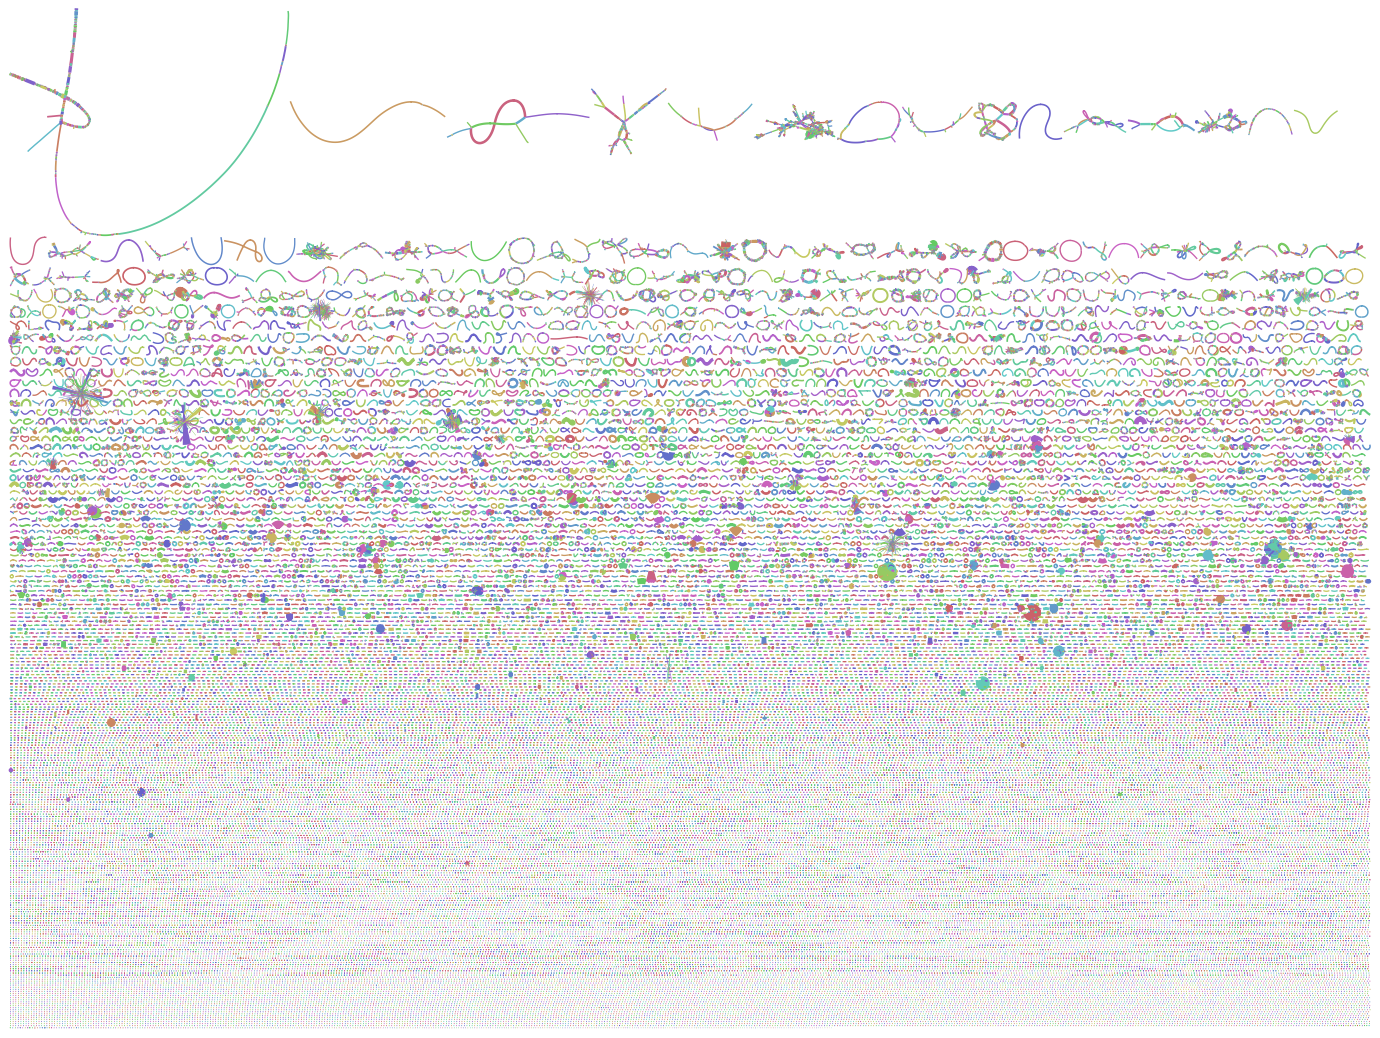
\includegraphics[width=1.0\textwidth]{Chapter3/Figs/svalbard_metagenome_minia_k51_m3_contigs_gfa.png}
  \caption[An arctic freshwater viral metagenome]{
    An arctic freshwater viral metagenome visualized with Bandage.
  }
  \label{fig:viral_metagenome_bandage}
\end{figure}

As expected given the small genome size of most viruses, the graph contains many small components (figure \ref{fig:viral_metagenome_bandage}).
The graph also contains a few large components, and many of the medium sized components are circular, which is expected given the nature of many DNA viruses.
Some components are topologically complex, which can be seen in figure \ref{fig:viral_metagenome_bandage} as ``hairball'' like structures.
When using $k=31$, indexing and alignment against the graph were impossible without a high-degree filter which removed nodes in such regions, however in the case of $k=51$ it is possible to index with only standard pruning of the DBG.

I held out 100,000 reads from the input to the assembly graph.
To evaluate the utility of using this graph as a reference for alignment, I aligned these 100,000 reads using {\tt vg map} and {\tt bwa mem} to the assembly graph and linear contig set respectively.
Although both methods mapped ~96\% of the reads, {\tt vg} had an average identity score of 95\% compared to 87\% for {\tt bwa}, reflecting that the {\tt bwa} alignments in many cases are not full length while those of {\tt vg} are. Furthermore, many reads mapped with higher scores (longer matches) to the graph than to the contig set (figure \ref{fig:viral_metagenome_scatter}).

\begin{figure}[htbp!]
  \centering
  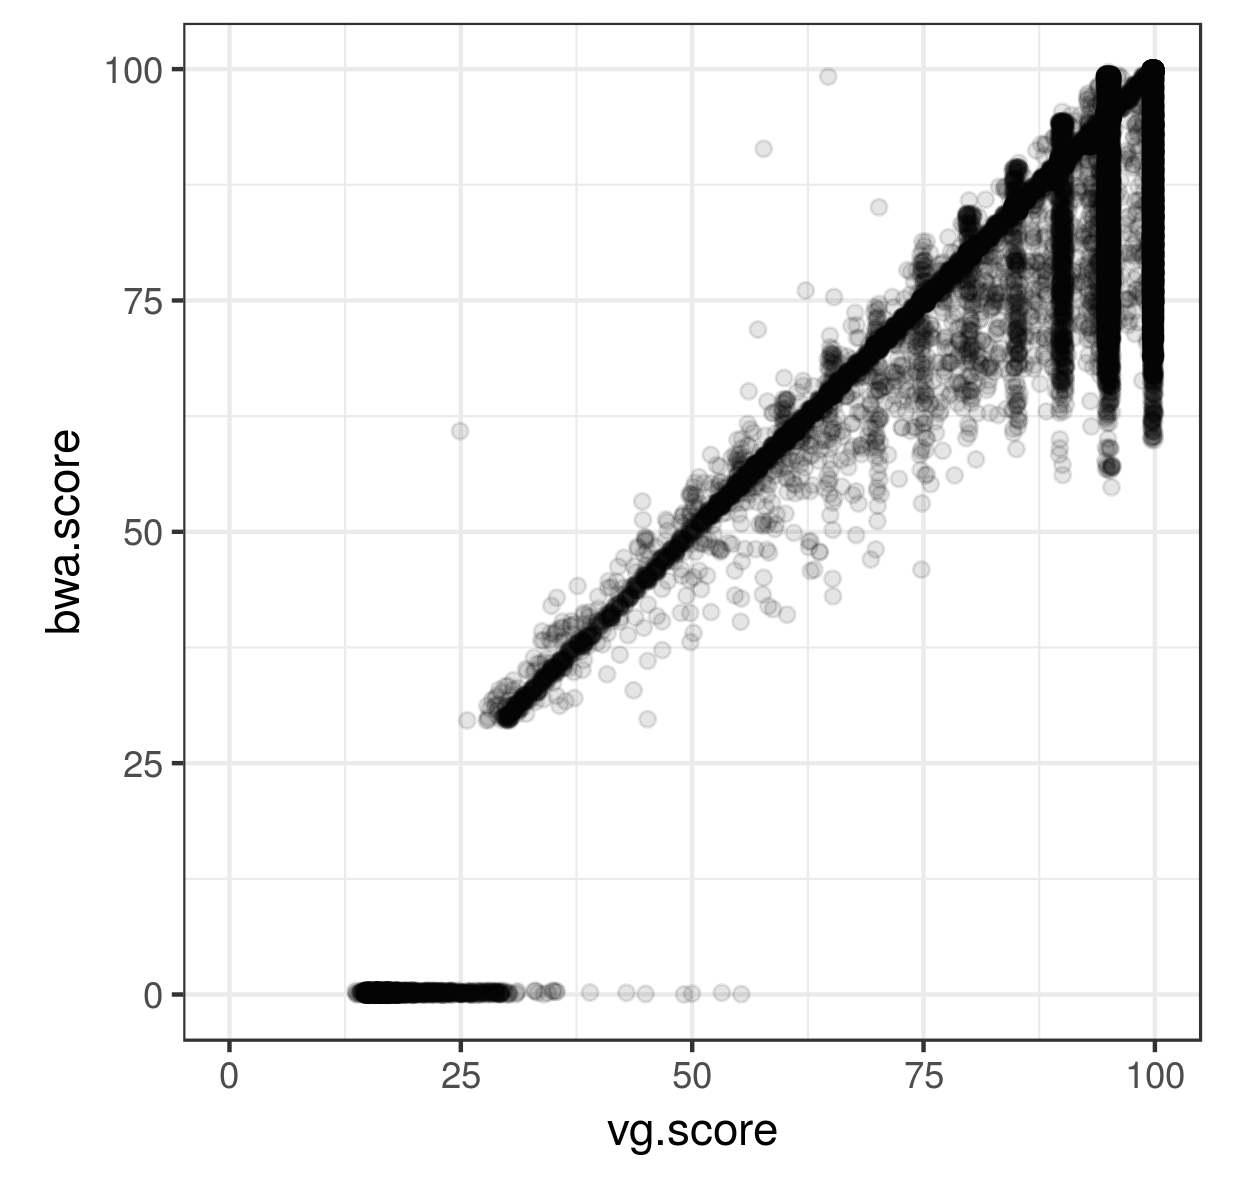
\includegraphics[width=0.7\textwidth]{Chapter3/Figs/ERR414817_holdout_bwa_vs_vg_k51_m3.png}
  \caption[Comparing {\tt vg} and {\tt bwa} alignment to the viral metagenome]{
    Comparison of alignment score between {\tt vg map} and {\tt bwa mem} when aligning against the pangenome graph or assembled contig set of the graph.
  }
  \label{fig:viral_metagenome_scatter}
\end{figure}

\subsection{Human gut microbiome}

As a counterpoint to the viral metagenomic sample used in the previous section, here I present a similar analysis based on a predominantly bacterial human gut microbiome obtained from a stool sample\footnote{Sample described at \url{https://portal.hmpdacc.org/cases/3674d95cd0d27e1de94ddf4d2e0398c4}, with data from \url{http://downloads.hmpdacc.org/data/Illumina/PHASEII/stool/SRS105153.tar.bz2}.} as part of the Human Microbiome Project (HMP) \cite{turnbaugh2007human,peterson2009nih}.

As with other assembly graph based analyses, I applied {\tt minia} with $k=51$ and a minimum abundance filter of 3 to the 29GB of compressed FASTQs from this sample.
The resulting assembly graph is shown in figure \ref{fig:human_gut_microbiome_bandage}.
It contains 144,829,925bp of sequence in 4,788,652 nodes and 4,665,919 edges, and as with other DBG assemblies I have discussed is locally linear.
Building and indexing the graph took around an hour on the 32vCPU/256GB server used in other experiments, and yielded a 74MB {\tt vg} graph with a 403MB {\tt xg} index and 606MB {\tt GCSA2} index, which was built with pruning with a 3 edge crossing limit in $k=16$.

\begin{figure}[htbp!]
  \centering
  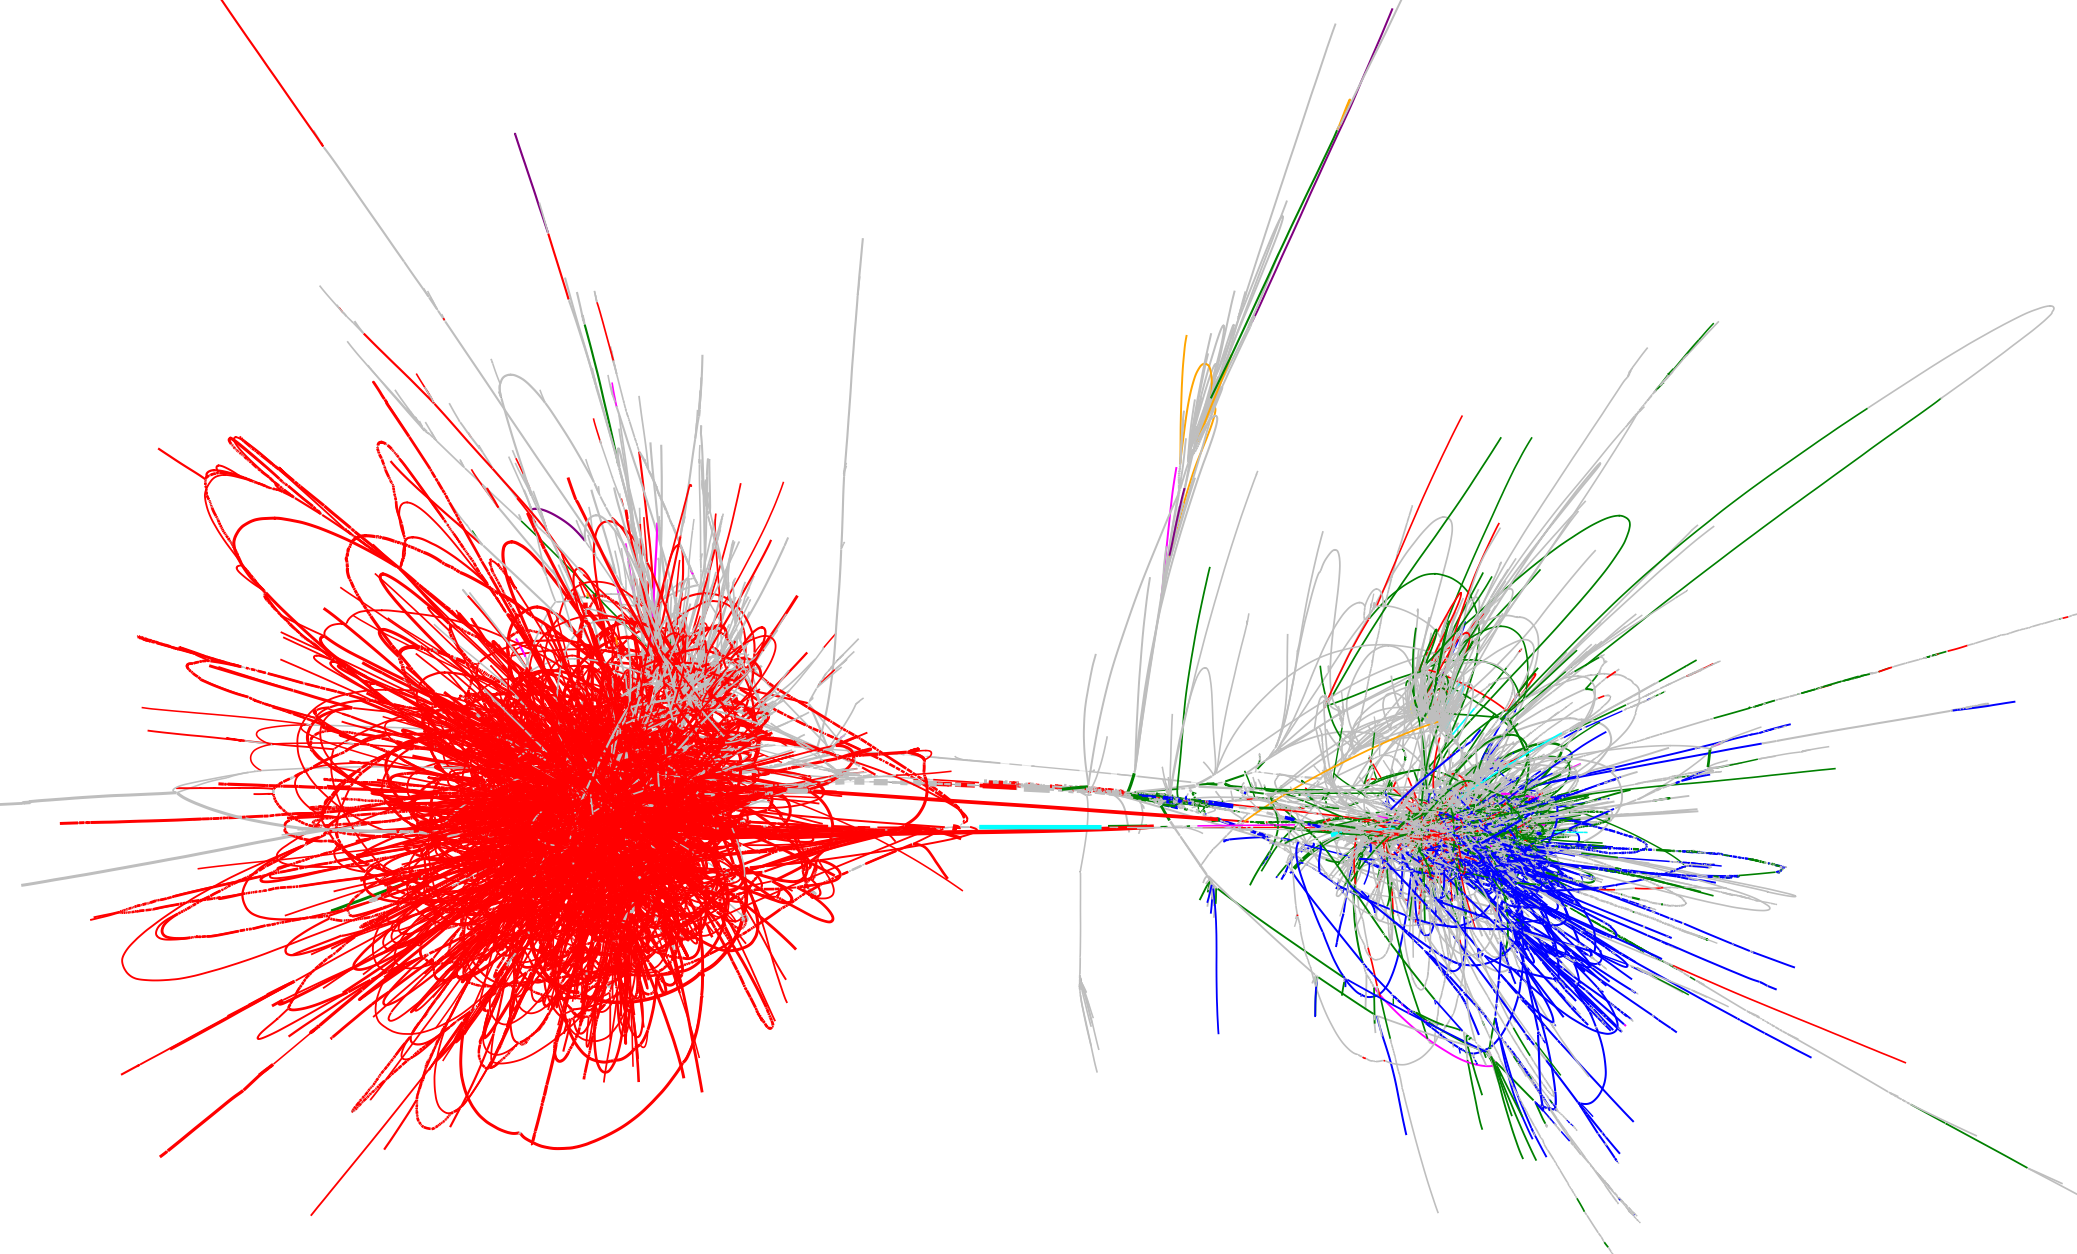
\includegraphics[width=1.0\textwidth]{Chapter3/Figs/human_gut_microbiome_phyla_colored_full_between.png}
  \caption[A human gut microbiome]{
    The largest components in a human gut microbiome assembly graph.
    Node width shows coverage in the assembly.
    Nodes that match to RefSeq genomes for nine given phyla are colored in the graph as described here with abundances: \emph{Bacteroides} (red) 34827, \emph{Clostridium} (green) 9521, \emph{Faecalibacterium} (blue) 5921, \emph{Bifidobacterium} (magenta) 373, \emph{Enterococcus} (cyan) 73, \emph{Enterobacter} (orange) 25, \emph{Klebsiella} (purple) 21, \emph{Escherichia} (yellow) 17, and \emph{Enterobacteriaceae} (brown) 2.
  }
  \label{fig:human_gut_microbiome_bandage}
\end{figure}


Human gut flora are primarily comprised of two main phyla, the Firmicutes and the Bacteroidetes \cite{mahowald2009characterizing}.
We can observe their presence in this sample in the structure of this assembly graph.
By aligning the node sequences in the graph against a subset of RefSeq Genomes which are commonly found in the human git microbiome, I verify that the two ends of dumbbell-like main component of the graph (figure \ref{fig:human_gut_microbiome_bandage}) represent these phyla.
The connection between them may be generated by horizontal transfer of genes or spurious correlation due to recurrent $k$-mers in the assembly graph, and it is notable that many of the nodes in the bridge between the two components show a high depth in the assembly graph, as shown by the node width in the figure.
\emph{E. coli} can be found on a small component connected to this bridge, shown at the top middle of the rendering.

\begin{figure}[htbp!]
  \centering
  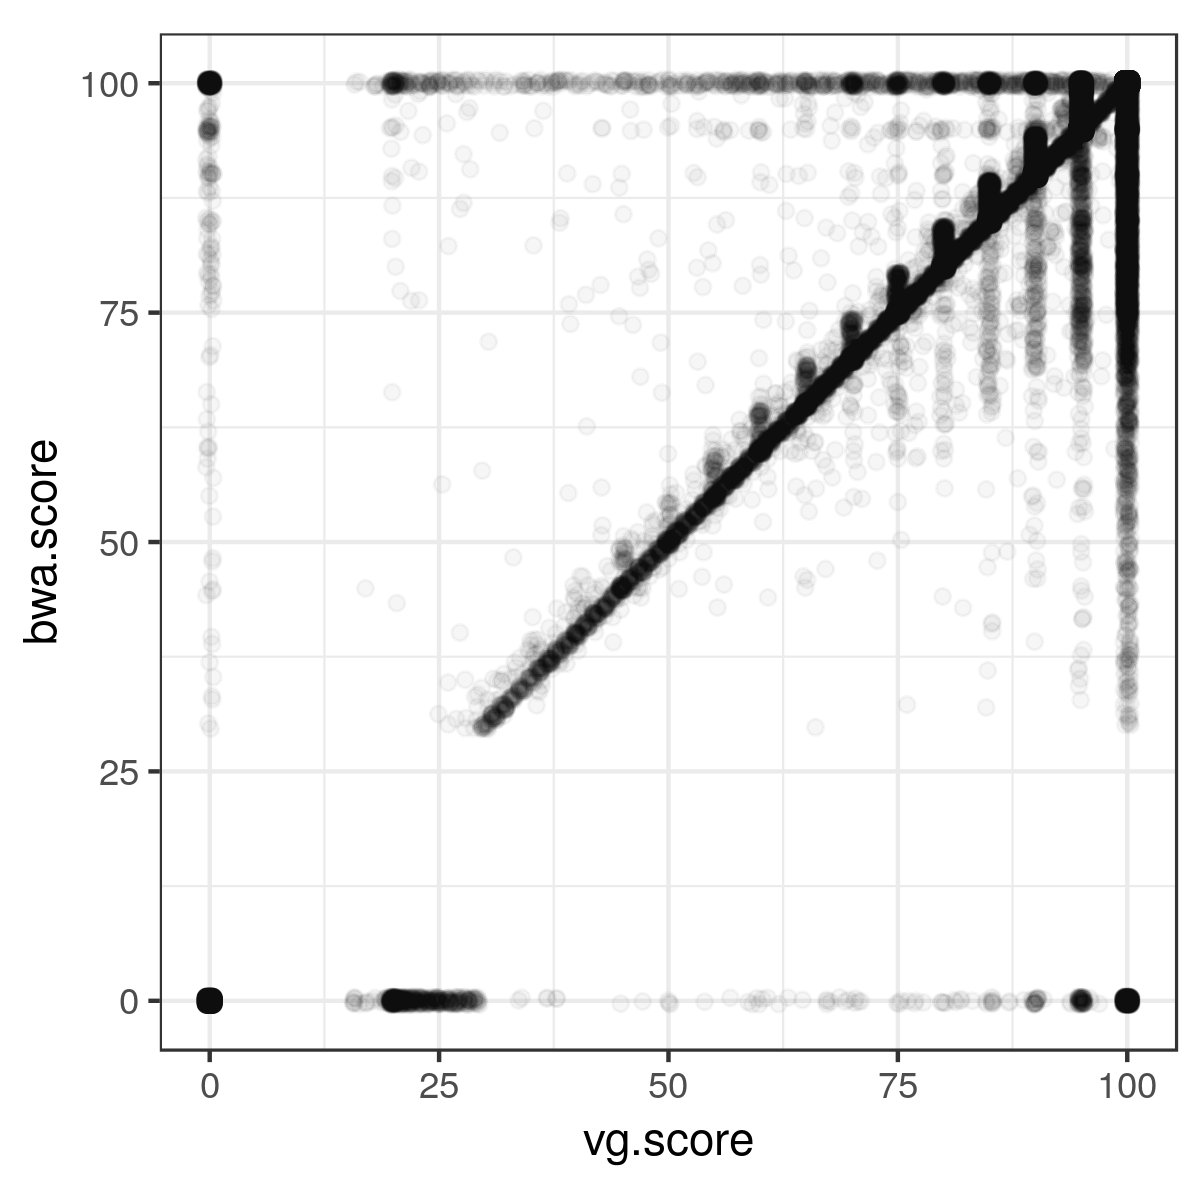
\includegraphics[width=0.7\textwidth]{Chapter3/Figs/human_gut_microbiome_SRS105153_holdout_vg_vs_bwa_scatter.png}
  \caption[Human gut microbiome alignment comparison]{
    Comparing alignment performance between {\tt vg map} and {\tt bwa mem} to the human gut microbiome assembly graph or its contigs.
  }
  \label{fig:human_gut_microbiome_scatter}
\end{figure}

To evaluate the utility of this graph for read alignment, I aligned 100k of the held-out reads with {\tt vg map} and {\tt bwa mem} to the graph and the contig set respectively.
This contig set would appear to be more suited to use as a linear reference and {\tt bwa mem} alignment than the viral metagenome in described in the previous section.
Alignment to the graph marginally improves the number of aligned reads, with {\tt bwa mem} aligning 95.7\% of them and {\tt vg map} aligning 96.3\%.
Overall, we can observe a similar level of change in the alignment score, with {\tt vg}'s mean score at 92.5 and {\tt bwa}'s at 92.0, which is a small but significant difference (two-tailed $T$-test $p=3.62\times 10^{-7}$).
The longer length of contigs in this graph and the lack of small circular contigs apparently contribute to the reduction in relative improvement offered by alignment to the graph in this bacterial context.
A scatterplot of alignment scores between the two methods reveals a slight shift in density below the diagonal in {\tt vg}'s favor (figure \ref{fig:human_gut_microbiome_scatter}).
It is possible that an assembly designed to capture more variation in the strains might benefit more greatly from the use of {\tt vg}.
A number of issues appear when inspecting these results, for instance that {\tt vg} does not align some reads that {\tt bwa} does.
This could represent a bug in the aligner or the effect of pruning on the gut metagenome graph's GCSA2 index.
We can conclude that while this method shows promise in a variety of metagenomic applications, improvements may be required for it to yield benefits in some contexts.


\section{RNA-seq}
%*0.5p 0.5h*

As described in section \ref{sec:rna_seq}, graphs have been used as a description of transcriptomes.
A transcript graph can encode alternatively spliced transcripts in a DAG.
By recording the transcripts as paths in this graph we can build a coherent annotation describing all the known transcripts and their sequences, and by indexing the graph with {\tt vg} we can align RNA-seq reads directly to it.
To build a splicing graph in {\tt vg} requires a linear reference and a gene model encoded in GFF, and uses the $edit$ function to augment the graph with alignments representing each gene annotation, thus incorporating edges for each spliced intron (section \ref{sec:construct_from_gff}).

\subsection{Yeast transcriptome graph}
%*1p 2h*

An obvious application of {\tt vg} is to the direct alignment of reads to a splicing graph.
I have only begun to explore this at the end of my studentship.
Once again, I started with yeast, which has only a small number (~280) of spliced genes.
I built a gene model graph (SGD+CDS) using the yeast reference genome from the Saccharomyces Genome Database (SGD) and its gene annotations\footnote{I used the 20150113 release from \url{https://downloads.yeastgenome.org/sequence/S288C_reference/genome_releases/S288C_reference_genome_R64-2-1_20150113.tgz}.}.
At 8.8MB, the serialized SGD+CDS {\tt vg} graph itself is only slightly larger than the SGD linear reference graph, which is 7.3MB.
However, its {\tt xg} index is much larger, 642MB, in contrast to the linear index at 38MB.
This index suffers a large penalty for the ~5000 embedded transcript annotations, as each becomes a full reference path, usable in alignment for positional inference.
To verify that the splicing graph would allow reads to align full length across splice junctions, I aligned 100k reads from a yeast mRNA sequencing data set\footnote{SRR2069949 in SRA, \url{https://www.ncbi.nlm.nih.gov/sra/?term=SRR2069949}}.

The low rate of alternative splicing in yeast means that only a handful of reads map across splice junctions encoded in the graph, but those that do now align full length, as seen in figure \ref{fig:yeast_rnaseq}.
The difference in aggregate alignment identity is small (0.91 vs 0.912) but marginally significant (two-tailed $T$-test $p=0.03927$).
This provides a basic proof of principle that the splicing graph can be represented as a variation graph and that {\tt vg} can align reads to it without any particular RNA-specific considerations.
Due to time constraints I was unable to further explore this topic.
One major concern was the runtime and memory costs to construct the {\tt xg} index.
These suggest that it may not be possible to build a splicing graph for a large genome with the transcripts encoded as positional paths, which further implies that improvements in the approximate positional metric in the graph will be required to scale RNA-seq alignment with {\tt vg}.
Further, the results shown in figure \ref{fig:yeast_rnaseq} indicate that there may be a positional offset bug in the conversion of the GFF files representing the transcriptome into the graph.
In summary, future work will be required to explore the use of {\tt vg} for RNA-seq data.

\begin{figure}[htbp!]
  \centering
  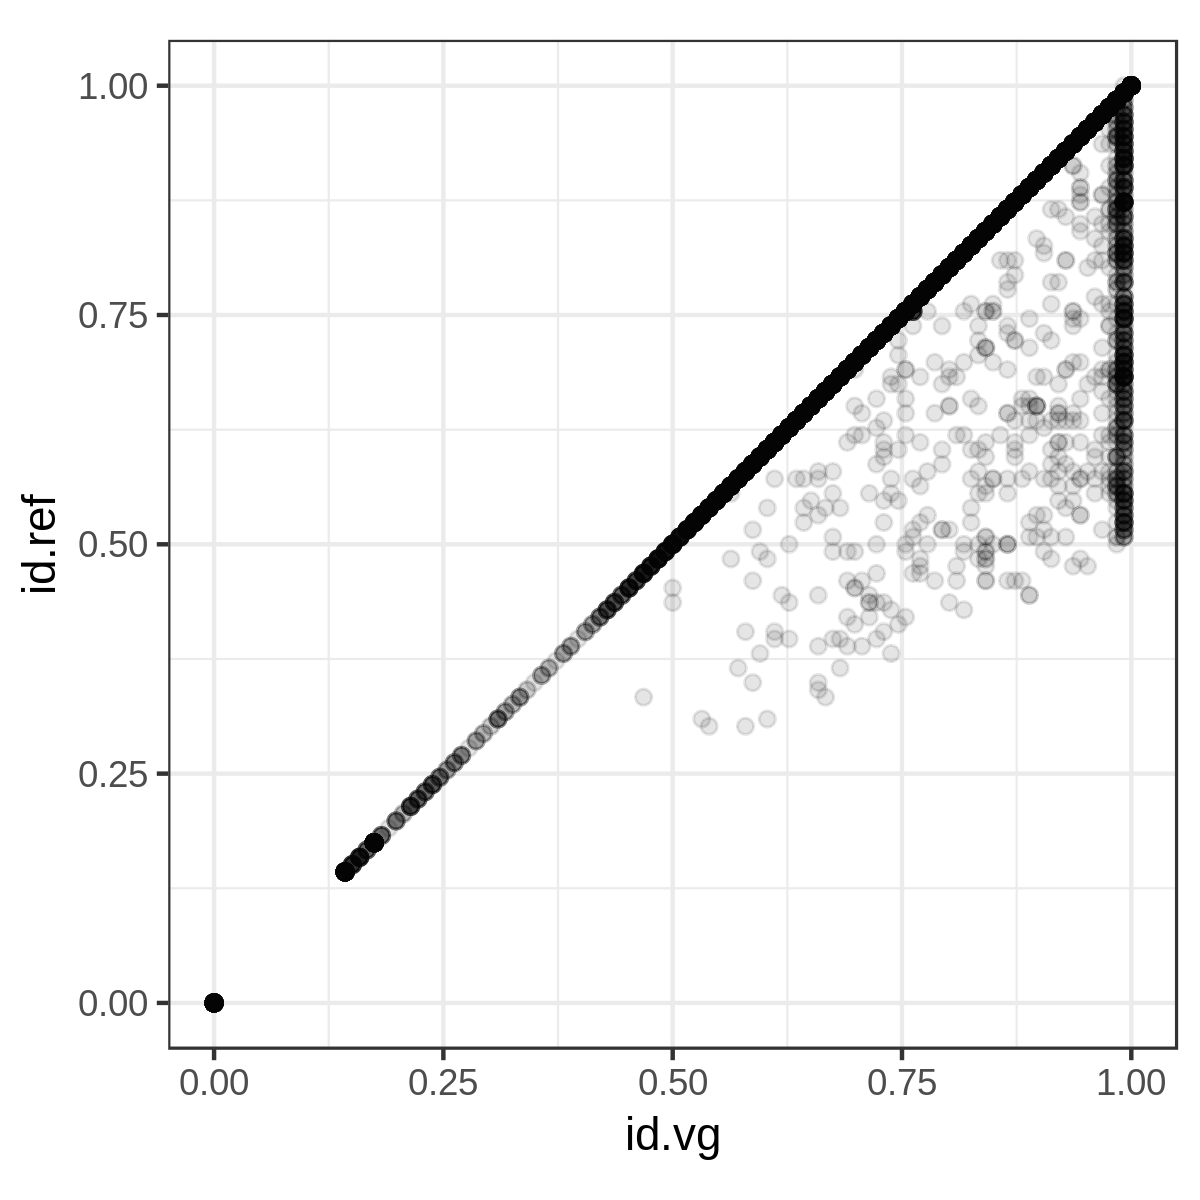
\includegraphics[width=0.7\textwidth]{Chapter3/Figs/SRR2069949_100k_ref_vs_gene_model.png}
  \caption[Aligning reads against the yeast transcriptome]{
    Comparing alignment identity between {\tt vg map} on the linear SGD reference ($y$-axis) and the SGD reference augmented by the transcripts in the annotated CDS ($x$-axis).
   }
  \label{fig:yeast_rnaseq}
\end{figure}

%\section{Applications that I contributed to}

% ...
